% ==== BEGIN OF PREAMBLE =======================================================
% ---- document class (use appropriate driver for DIV to PS/PDF conversion):
\documentclass[12pt,a4paper]{book}


% ---- graphicx package:
\usepackage{graphicx}

% ---- colors
\usepackage{xcolor}


% ---- natbib package:
\usepackage{natbib}
\bibpunct{(}{)}{;}{a}{}{,}  % adjust author-year citation format 


% ---- hyperref package for cross-references:
\usepackage{hyperref}
% -- USE BLACK LINKS IN PRINTOUT (uncomment the following lines if necessary):
%\hypersetup{colorlinks,%
%            linktocpage,%
%            breaklinks,%
%            citecolor=black,%
%            filecolor=black,%
%            linkcolor=black,%
%            urlcolor=black,}
% -- use color links in pdf version (comment the following lines if necessary):
\hypersetup{colorlinks,
            linktocpage,%  make page number, not text, be link on TOC, LOF & LOT
            breaklinks,%
            citecolor=blue,%
            filecolor=blue,%
            linkcolor=blue,%
            urlcolor=blue,}


% ---- caption package:
\usepackage[font=small,labelfont=bf]{caption}

% ---- math bold package and other maths packages
\usepackage{amsmath}
\DeclareMathOperator*{\argmin}{\arg\min}
\DeclareMathOperator*{\argmax}{\arg\max}
\usepackage{bm}
\usepackage{amssymb}

% ---- multirow
\usepackage{multirow}

% ---- clever referencing
\usepackage[capitalise]{cleveref}
\crefformat{footnote}{#2\footnotemark[#1]#3}


% ---- subfigure package:
\usepackage[tight,nooneline,FIGTOPCAP,bf]{subfigure}
% \setlength{\subfigcaptopadj}{-6pt}  % vertical position of subfigure labels
\renewcommand{\thesubfigure}{\alph{subfigure}}
\makeatletter
    \renewcommand{\@thesubfigure}{(\thesubfigure)}  % subfigure labels:     (a)
    \renewcommand{\@@thesubfigure}{\thesubfigure}   % produced by \subref:   a
    \renewcommand{\p@subfigure}{\thefigure}         % produced by \ref:   3.1a
\makeatother


% ---- fancyhdr package:
\usepackage{fancyhdr}


% ---- some other useful packages:
% \usepackage{showkeys}  % show all keys (labels)
% \usepackage{times}     % use times new roman instead of computer modern font


% ---- page layout:
\setlength{\textheight}{24cm}
\setlength{\textwidth}{15cm}
\setlength{\topmargin}{-0.9cm}
\setlength{\headheight}{0.6cm}
\setlength{\headsep}{1cm}
\setlength{\footskip}{1cm}
\setlength{\oddsidemargin}{9.1mm}
\setlength{\evensidemargin}{-0.2mm}
\setlength{\marginparwidth}{2cm}


% ---- paragraph and line properties:
\setlength{\parindent}{0.8cm}
\setlength{\parskip}{0pt}
\linespread{1.2}
\sloppy % reduce number of word divisions and use more space between words


% ---- header format: use fancyhdr page style:
\pagestyle{fancy}
\fancyhf{}
\renewcommand{\chaptermark}[1]{\markboth{#1}{}}
\renewcommand{\sectionmark}[1]{\markright{\thesection\ #1}}
\fancyhead[LE,RO]{\thepage}
\fancyhead[LO]{\slshape \small \rightmark}
\fancyhead[RE]{\slshape \small \leftmark}
\renewcommand{\headrulewidth}{0pt}


% ---- define label format for equations, figures, and tables:
\renewcommand{\theequation}{\thechapter.\arabic{equation}}
\renewcommand{\thefigure}{\thechapter.\arabic{figure}}
\renewcommand{\thetable}{\thechapter.\arabic{table}}

% ---- tikiz stuff for U-Net picture
\usepackage{import}
\usepackage{tikz}
\subimport{./layers/}{init}
\usetikzlibrary{positioning}

\def\ConvColor{rgb:yellow,5;red,2.5;white,5}
\def\ConvReluColor{rgb:yellow,5;red,5;white,5}
\def\PoolColor{rgb:red,1;black,0.3}
\def\UnpoolColor{rgb:blue,2;green,1;black,0.3}
\def\FcColor{rgb:blue,5;red,2.5;white,5}
\def\FcReluColor{rgb:blue,5;red,5;white,4}
\def\SoftmaxColor{rgb:magenta,5;black,7}


\newcommand{\copymidarrow}{\tikz \draw[-Stealth,line width =0.8mm,draw={rgb:blue,4;red,1;green,1;black,3}] (-0.3,0) -- ++(0.3,0);}



% ==== END OF PREAMBLE =========================================================


% ==== BEGIN OF BODY ===========================================================
\begin{document}


% ==== START FRONT MATTER (use ROMAN numerals) =================================
\frontmatter


% ==== TITLE PAGE ==============================================================
% ---- include tex-file (CHOOSE APPROPRIATE FILE):
\begin{titlepage}
\begin{center}

% ---- main title
~\\[15mm]
{\Huge  {\bf Precipitation Nowcasting:}}\\[5mm]


% ---- subtitle (if necessary):
{\LARGE {\bf a Deep Learning Approach}}\\[15mm]


% ---- type of thesis:
{\Large \textsc{Master's Thesis}} \\[15mm]


% ---- field of study:
{\large in Environmental Meteorology} \\[15mm]


% ---- institution:
{\large Submitted to the} \\[2mm]
{\Large \textsc{Faculty of Geo- and Atmospheric Sciences}} \\[2mm]
{\large of the} \\[2mm]
{\Large \textsc{University of Innsbruck}} \\[15mm]


% ---- degree:
{\large in Partial Fulfillment of the Requirements for the Degree of} \\[2mm]
{\Large \textsc{Master of Science}} \\[15mm]


% ---- author:
{\large by} \\[2mm]
{\Large \textsc{Stefano Campostrini}} \\[15mm]


% ---- advisor:
{\large Advisor} \\[2mm]
{\large Univ.-Prof. Dr. Georg Mayr} \\[15mm]


% ---- location, date:
{\large Innsbruck, May 2022}


\end{center}
\end{titlepage}
    % activate this line for Master's Thesis
% \begin{titlepage}
\begin{center}

% ---- main title
~\\[15mm]
{\Huge  {\bf A Template for a Science Thesis:}}\\[5mm]


% ---- subtitle (if necessary):
{\LARGE {\bf Scientific Writing in \LaTeXe{}}}\\[15mm]


% ---- type of thesis:
{\Large \textsc{Diploma Thesis}} \\[15mm]


% ---- field of study:
{\large in Meteorology} \\[15mm]


% ---- institution:
{\large Submitted to the} \\[2mm]
{\Large \textsc{Faculty of Geo- and Atmospheric Sciences}} \\[2mm]
{\large of the} \\[2mm]
{\Large \textsc{University of Innsbruck}} \\[15mm]


% ---- degree:
{\large in Partial Fulfillment of the Requirements for the Degree of} \\[2mm]
{\Large \textsc{Master of Natural Science}} \\[15mm]


% ---- author:
{\large by} \\[2mm]
{\Large \textsc{FirstName LastName}} \\[15mm]


% ---- advisor:
{\large Advisor} \\[2mm]
{\large Univ.-Prof. Dr. Hans Ertel} \\[15mm]


% ---- location, date:
{\large Innsbruck, December 2009}


\end{center}
\end{titlepage}
   % activate this line for Diploma Thesis
\newpage
~\thispagestyle{empty}
\newpage
% ---- start page numbering again:
\setcounter{page}{1}


% ==== DEDICATION ==============================================================
% ---- include tex-file:
% \addcontentsline{toc}{chapter}{Dedication}
\thispagestyle{plain}

\begin{center}
 \Large\em\null\vskip5cm To all who have been close to me in this journey, especially from far away \\[3cm]
\end{center}

\newpage
\thispagestyle{plain}

% ==== ABSTRACT ================================================================
% ---- set some counters to zero:
\setcounter{equation}{0}
\setcounter{table}{0}
\setcounter{figure}{0}
% ---- include tex-file:
\chapter*{Abstract}
\addcontentsline{toc}{chapter}{Abstract}
\thispagestyle{plain}

Forecasting precipitation at very short lead times is a task that is difficult to address through numerical weather prediction models due to the great amount of computing power required to solve the physical equations that govern the behaviour of the atmosphere in a timely fashion. The advances in the field of deep learning and the large amount of historical data of radar precipitation maps that are openly available make the precipitation nowcasting problem a good candidate for deep learning solutions. To assess the potential of the U-Net neural network architecture at the 1hr time scale a comparison is made of its performance to persistence, i.e. the assumption that the prediction is equal to the last available frame. The problem is structured as a multi-class classification task over 4 precipitation intensity classes. The model takes 6 input images of 1h cumulative precipitation of the RW product from the RADar Online ANeichung (RADOLAN) dataset of the German weather service (DWD) and an area of 256km$\times$256km over northern Germany is selected. The task is to predict the precipitation classes of the pixels of the RADOLAN image at 6h from the first input image. It is found that the model performs better than persistence at higher precipitation rates. For rainfall rates in [0mm/h, 0.1mm/h) the model has a Critical Success Index (CSI) of 0.853 compared to 0.893 of persistence. For rainfall rates in [0.1mm/h, 1mm/h), [0.1mm/h, 1mm/h) and [0.1mm/h, $\infty$mm/h) the model has better CSI than persistence (0.292 vs 0.276, 0.253 vs 0.182 and 0.191 vs 0.128 respectively). For the same classes the Heidke Skill Score (HSS) absolute performance diminishes with increasing precipitation rate but gets better relative to persistence (0.579 vs 0.583, 0.438 vs 0.441, 0.404 vs 0.314 and 0.321 vs 0.229). Finally, both a higher average HSS for the model compared to persistence (0.436 compared to 0.392) and a higher average CSI (0.397 compared to 0.370) are found. A visual inspection of the predictions suggests that the neural network is able to infer the general structure of the precipitation field but has a tendency to predict higher rain rates. It can be concluded that the results are encouraging and that the application of the U-Net architecture to 1h cumulative precipitation maps should be further investigated.

\newpage
\thispagestyle{plain}


% ==== TABLE OF CONTENTS =======================================================
~
\newpage
\addcontentsline{toc}{chapter}{Contents}
\tableofcontents
\newpage
\thispagestyle{plain}


% ==== START MAIN MATTER (use ARABIC numerals) =================================
\mainmatter


% ==== INTRODUCTION (CHAPTER 1) ================================================
% ---- set some counters to zero:
\setcounter{equation}{0}
\setcounter{table}{0}
\setcounter{figure}{0}
% ---- include tex-file:
\chapter{Introduction}\label{chap1}
\thispagestyle{plain}

% ====SECTION 1 ================================================================
\section{Motivation}
Current weather forecasts are based on global numerical weather prediction (NWP) models that solve the governing physical equations of the atmosphere to predict its future states. If the forecast happens for very short time-frames in the order of a couple of hours to, according to some authors, 6 hours, the forecast is referred to as nowcast. However, for these time-frames, numerical methods of predicting the weather are bound by the incredible amount of computing power required leading to a necessary trade-off between timeliness of the prediction and spatial resolution. For instance the High-Resolution Rapid Refresh model (HRRR) is a National Oceanic and Atmospheric Administration (NOAA) atmospheric model with 3km spatial resolution updated hourly \citep{NOAA2021} that covers the extension of the United States. 

For predicting variables of high interest to the public such as spatial precipitation distribution, optical flow algorithms are currently being used for time horizons from 1h to 4h. These algorithms use geometrical features in the input images and their spatial movement -- for instance by using radar reflectivity maps -- to extrapolate their position at future timestamps.

The governing equations of the physical processes behind the behaviour of the atmosphere are of a non-linear nature. This suggests that non-linear statistical models such as artificial neural networks -- that abstract features from a historical dataset -- would be able to represent these processes. Deep learning -- i.e. neural networks with many hidden layers -- has recently become a plausible method of predicting physical processes mainly driven by historical-data availability and reduced cost of the devices used for the relevant computations (Graphics Processing Units or GPUs).

Given the historical archives of radar precipitation maps it is clear that deep learning could be applied to the precipitation nowcasting problem. A significant point in favor of investigating this approach is that, after the moderately low cost of the training of a deep neural network model, the production of predictions (also called inferences) are characterized by both an incredibly low cost and very short time frames (in the order of 1sec). So much so that this can even happen consumer-grade GPUs. This properties satisfy the timeliness requirement of precipitation nowcasting.

%Precipitation impacts on society in terms of cost and life.
%Importance of forecasting it.
%Methods of forecast.
%Recently deep learning in geophysical sciences.
%Advantages and Disadvantages of these methods.
%Need to investigate Deep learning approach because of very low cost of inference and a great availability of data.
% ==== SECTION 2 ===============================================================
\section{State of the Art}\label{1sec:2}
Artificial neural networks find their origin in \citet{McCulloch1943AActivity} where the authors describe them as having thresholds and weights finding that, in principle, a neural network could compute every function that a physical computer is able to compute. \citet{Rosenblatt1958TheBrain} proposed the first trainable neural network. The perceptron -- as it is called -- has all the characteristics of modern day neural networks except that it is very simple in its design. From this original design the multi-layer perceptron has become the standard artificial neural network. It is also known as fully-connected feed-forward neural network and is fundamentally made of units grouped into layers. The information flows from the input layer to the output layer passing through the (hidden) layers in-between. The units in a layer take as input the signals from all the units of the layer before them, they weight them according to specific weights that are subject to optimization, apply a non-linear function acting as threshold and finally pass on a value to all the units of the following layer until the signal reaches the output unit. Neural networks have found many applications throughout the sciences due to their versatility in finding statistical relations. Their main drawbacks are the design -- no canonical designs exist for a given task -- the search for the right combination of parameters governing the behaviour of the model (also called hyperparameters) and the computational demands compared to other statistical methods.

Deep learning has been used in the physical sciences for predictions spanning the entire field for quite some time now, mainly led by the general advances of the machine learning field. A clear example of the use of deep learning in the Earth sciences is \citet{Steffenel2021ForecastingExperiment} where a deep neural network forecasted O3 advection. \citet{Reichstein2019DeepScience} give a thorough overview of deep learning in Earth Sciences.

As it pertains to the particular task of predicting the weather, many approaches have been proposed for a variety of different tasks. Using deep learning methods to forecast future states of the atmosphere is also called deep learning weather prediction (DLWP). \citet{Ren2021DeepSurvey} propose three different groupings for the architectures that solve weather prediction problems. (1) those based on well known architectures from the general literature, such as autoencoders \citep{Lin2018DynamicForecast,Hossain2015ForecastingApproach}, convolutional neural networks \citep{Qiu2017ANetworks} or long-short-term memory networks \citep{Karevan2018Spatio-temporalForecasting}, (2) hybrid architectures composed of a combination of those in (1), (3) a union of deep neural networks with NWP models to join the benefits of both theory-driven and data-driven approaches.

In the specific case of precipitation nowcasting, many different solutions have been employed (see \citet{Ren2021DeepSurvey} for a survey of the current methods).

% Forecasting radar images using past snapshots is a problem called video prediction - well known in the general Artificial Intelligence literature. Hence, some methods used come directly from the field.

\citet{Shi2015ConvolutionalNowcasting} propose a convolutional long-short-term memory (ConvLSTM) network for precipitation nowcasting that consists of a combination of convolutional and LSTM network structures. However, a main drawback is that as structured, it is location invariant. For this reason \citet{Shi2017DeepModel} propose the trajectory grated recurrent unit (TrajGRU) model that adds the ability for the model to actively learn the structure of natural motion and transformation which is location-dependent. This kind of model has been shown to perform exceptionally well for time-series predictions as the recurrent structure implicitly assumes a chaining of past and future events of the series. \citet{Wang2017PredRNN:LSTMs,Wang2018PredRNN++:Learning} also adopt variations of the LSTM core structure proposing the predictive recurrent neural network (PredRNN) and the improvement PredRNN++ respectively. \citet{Wang2018ApplicationNowcasting} successfully applies them to the task of precipitation nowcasting.

Google Research \citet{Agrawal2019MachineImages,Snderby2020MetNet:Forecasting} were both able to successfully apply DLWP to precipitation now-casting even surpassing NOAA's HRRR model. The U-Net architecture, used in \citet{Agrawal2019MachineImages} and \citet{Ayzel2020RainNetNowcasting}, is directly inspired from the well known model introduced in \citet{Ronneberger2015U-Net:Segmentation} and operate with radar precipitation images at 10min and 5min intervals respectively. With the implementation of skip connections \citep{He2016DeepRecognition,He2016IdentityNetworks}, this model gave good results in both applications to precipitation nowcasting. The main idea behind this type of architecture is the division of the network into two distinct parts, the encoder and the decoder. The first part is responsible for abstracting features that, with increasing depth, become more high-level. The second part of the network tries to rebuild a plausible image by using more low-level features when the stream nears to the output layer.


%Different ways in which deep learning has been used in the physical sciences.
%Particular problem of radar image forecasting.
%Different approaches. (ways to read the problem)
%Main issues that have been found with the various approaches.
%What was found to be important for solving some of these issues.
%How did we come to use U-Net.
%Why 1 hourly. Most use 5 minutes.

% ==== SECTION 3 ===============================================================
\section{Goals and Outline}\label{sec:researchquestions}
The aim of this project is to investigate the use of deep learning with 1h cumulative data of precipitation in northern Germany with a U-Net architecture model inspired by \citet{Agrawal2019MachineImages}. Some intuitions from \citet{Ayzel2020RainNetNowcasting} are used. The U-Net is applied to a dataset of hourly cumulated precipitation amounts freely provided by the German weather service - Deutscher Wetterdienst (DWD). The model is tasked with predicting the future radar precipitation maps in the simplified form of 4 mutually exclusive precipitation classes by taking as input multiple continuously-valued precipitation maps for the preceding timestamps. This task is also known as multi-class classification or multi-class segmentation. To better understand the predictive power of the model, it is compared with the persistence benchmark. This benchmark consists of predicting a future state of the atmosphere by assuming it remains unchanged from the last available timestamp before the prediction. Albeit its simplicity, persistence predictions are not trivially easy to outperform. To facilitate the training process of the model, avoid overfitting and better the final results -- a process called regularization -- this project uses methods taken directly from the deep learning literature.
The thesis will address the following questions:
\begin{itemize}
\item[(1)] Does the employed neural network outperform persistence?
\item[(2)] How does model performance depend on the rainfall intensity?
\item[(3)] The model of \citet{Agrawal2019MachineImages} after which this project is inspired outperformed persistence for all precipitation classes. Can this result be confirmed?
\end{itemize}

The second and next chapter of this thesis covers the theoretical principles behind the production of radar precipitation maps, addresses the dataset used in the project and its pre-processing for the specific applications to the task addressed with the proposed model. It illustrates the workings of neural networks giving more attention to the components of the model architecture that are used in this project. Details are given on the deep learning regularization techniques that are later employed. Chapter three provides the results of the project. Finally, chapter four states the answers to the research questions, discusses and compares them with similar studies and suggests plausible developments and open questions.



\newpage
\thispagestyle{plain}


% ==== CHAPTER 2 ===============================================================
% ---- set some counters to zero:
\setcounter{equation}{0}
\setcounter{table}{0}
\setcounter{figure}{0}
% ---- include tex-file:
\chapter{Data and Methods}\label{chap2}
\thispagestyle{plain}


% ==== SECTION 1 ===============================================================
\section{Data}\label{2sec:1}
\subsection{Radar Principles}
Radar meteorological observations are of extreme importance for a multitude of variables. The main application of interest in this project is the use of radar for determining the precipitation amount through the so-called reflectivity.
The fundamental principle behind weather radars is the transmission of electromagnetic waves at a known wavelength (typically in the range of 3-10GHz) in the microwave range that are either absorbed or scattered and their subsequent detection. The emission power is in the order of $10^2$W - $10^3$W and the power received amounts to a mere $10^{-16}$kW hence a staggering 18 orders of magnitude. Another challenge for the receiver is the 9 orders of magnitude spanned by the incoming power depending on the difference in distance and type of possible targets that go from hail to dust.
The signal is emitted in a beam of approximately 1-2\textdegree  width. Many factors affect absorption and scattering of the incoming radiation such as shape, dielectrical properties of the targets and the ratio of the wavelength to the size of the particle doing the scattering. Scattering itself occurs at two different regimes, one for a high wavelength-to-size ratio and one for low wavelength-to-size ratio; In the {\textit{Rayleigh scattering regime}} -- which is the first of the two -- scattered energy goes with $D^6$ where $d$ is the diameter of the scatterer. {\textit{Mie scattering}} happens in the other case and the governing law is not a simple function of target size.

A very important quantity in radar observations is the so-called \textit{logarithmic reflectivity factor} expressed as
\begin{equation}
    Z = 10 \log_{10} \left( \dfrac{z}{1 \text{mm}^6/\text{m}^3}\right)
\end{equation}
with $z$ the reflectivity factor none other than the summation of target diameters to the sixth power, i.e.
\begin{equation}
    z = \int_0^{\infty} N(D)D^6 dD
\end{equation}
where $N(D)$ is the drop-size distribution considered to be a continuous function of drop size $D$.


Z is given in dBZ (decibels relative to $1\text{mm}^6/\text{m}^3$).
Reflectivity factor $z$ and received backscattered power $P_r$ are bound by
\begin{equation}
    z = C P_r r^2
\end{equation}
with a radar constant C dependent on the charachteristics of the radar, and $r$ the distance to the target.

Another important factor affecting backscattered power is attenuation, i.e. the absorption and scattering of the radar signal along the path to the target. This affects radars with $\lambda < 10\text{cm}$ the most. 

The signal wavelengths most commonly used for weather radar applications are in the S-Band ($7.5\text{cm} < \lambda < 15\text{cm}$) and C-Band ($3.75\text{cm} < \lambda < 7.5\text{cm}$). The US National Weather Service (NWS) employs a set of 160 S-band radars in the Nexrad (Next-Generation Radar) radar network. European weather services, on the other hand, mostly employ C-band radars.

The assignment of part of the incoming scattered signal to a specific range (or distance) from the radar is attained through a periodical sampling (every 0.1-1$\mu$s). The location of the sampled volume is readily determined by knowing azimuth angle, elevation angle and the distance from the antenna given by
\begin{equation}
    r = \dfrac{ct}{2}
\end{equation}
with $c$ being the speed of light and t the amount of time for the signal to arrive at the target scatterer volume and come back. Additional corrections should be made to account for the Earth's curvature and refraction - the refractive index is a strong function of the air density. In particular cases, such as when a strong temperature inversion is present, the beam can make contact with the ground through strong deflection.
\subsubsection{Z-R relationships}
The simplest relationship between logarithmic reflectivity factor Z and rainfall rate R is based on the assumption that
\begin{equation} \label{eq:zr}
    Z = A R^B
\end{equation}
with $A$ and $B$ being constants. Given a $D^6$ dependence of $Z$ and a $D^3$ dependence of $R$, without knowing the drop size distribution this method is prone to errors. Nonetheless, with reasonable assumptions (i.e. a Marshall-Pamer drop size distribution) one obtains 
\begin{equation}
    Z = 200 R ^{1.6}
\end{equation}
A correction to this relationship is made during the RADOLAN routine (RADar-OnLine-ANeichung \citet{DeutscherWetterdienst2022RADOLANANeichung}) -- see \cref{sec:radolan}. 

In addition to the uncertainties of A and B in \cref{eq:zr} due to not knowing the drop size distributions, other sources of errors for the correct determination of the rainfall rate include:
\begin{itemize}
    \item The inability to measure the reflectivity near the ground the further away from the radar site. Not only is there a normal increase in distance due to a slight angle of the radar beam with respect to the horizon ($\approx$0.8\textdegree), but the curvature of the earth also has a significant impact on the height reached by the beam.
    \item Attenuation of the beam due to orography
    \item Rainfall rate gradients
    \item Errors in the calibration of the radar
    \item The presence of hail, thus invalidating the Rayleigh scattering approximation
\end{itemize}

Rain gauges, however, measure the actual rainfall rate on the ground but only in the spot where they are located. The measured rainfall rate is therefore representative for a limited area. The RADOLAN procedure, described in the following section, combines the the real rainfall rates measured through the rain gauges with the radar obtained precipitation maps. The final product of this procedure is a precipitation map that retains the spatial characteristics of the precipitation distribution from the weather radars but has values closer to the ground truth compared to a precipitation map obtained only through the conversion of the radar reflectivity to the rainfall rates with a simple Z-R relationship.

\subsection{Radolan Dataset} \label{sec:radolan}
The German Weather Service (DWD - Deutsches Wetter Dienst) offers a variety of products derived from their deployed sensor suite of weather radars and rain gauges. One of these products is the timely online calibration of radar spatial precipitation distributions (RADOLAN - RADar-OnLine-ANeichung \citet{DeutscherWetterdienst2022RADOLANANeichung}) that are used to produce quantitative radar-nowcasting distributions (RADVOR - RADar - NiederschlagsVORhersage \citet{DeutscherWetterdienst2022RADVORRadar-Niederschlagsvorhersage}), as an input for the COSMO-DE Numerical Weather Prediction model and for the convection development model (KONRAD - KONvektion Entwicklung in RADarprodukten \citet{DeutscherWetterdienst2022KONRADRADarprodukten}).

\subsubsection{Sensor Field}
For the production of RADOLAN precipitation distribution maps the DWD employs 17 C-Band Radars that cover the entirety of Germany. These measure the precipitation rate indirectly by capturing the reflection of the radar signals by the hydrometeors above ground. \cref{fig:dwdradar} shows the map and the 150km ranges of the various Weather Radars of the DWD. 

\begin{figure}[h!]
    \centering
    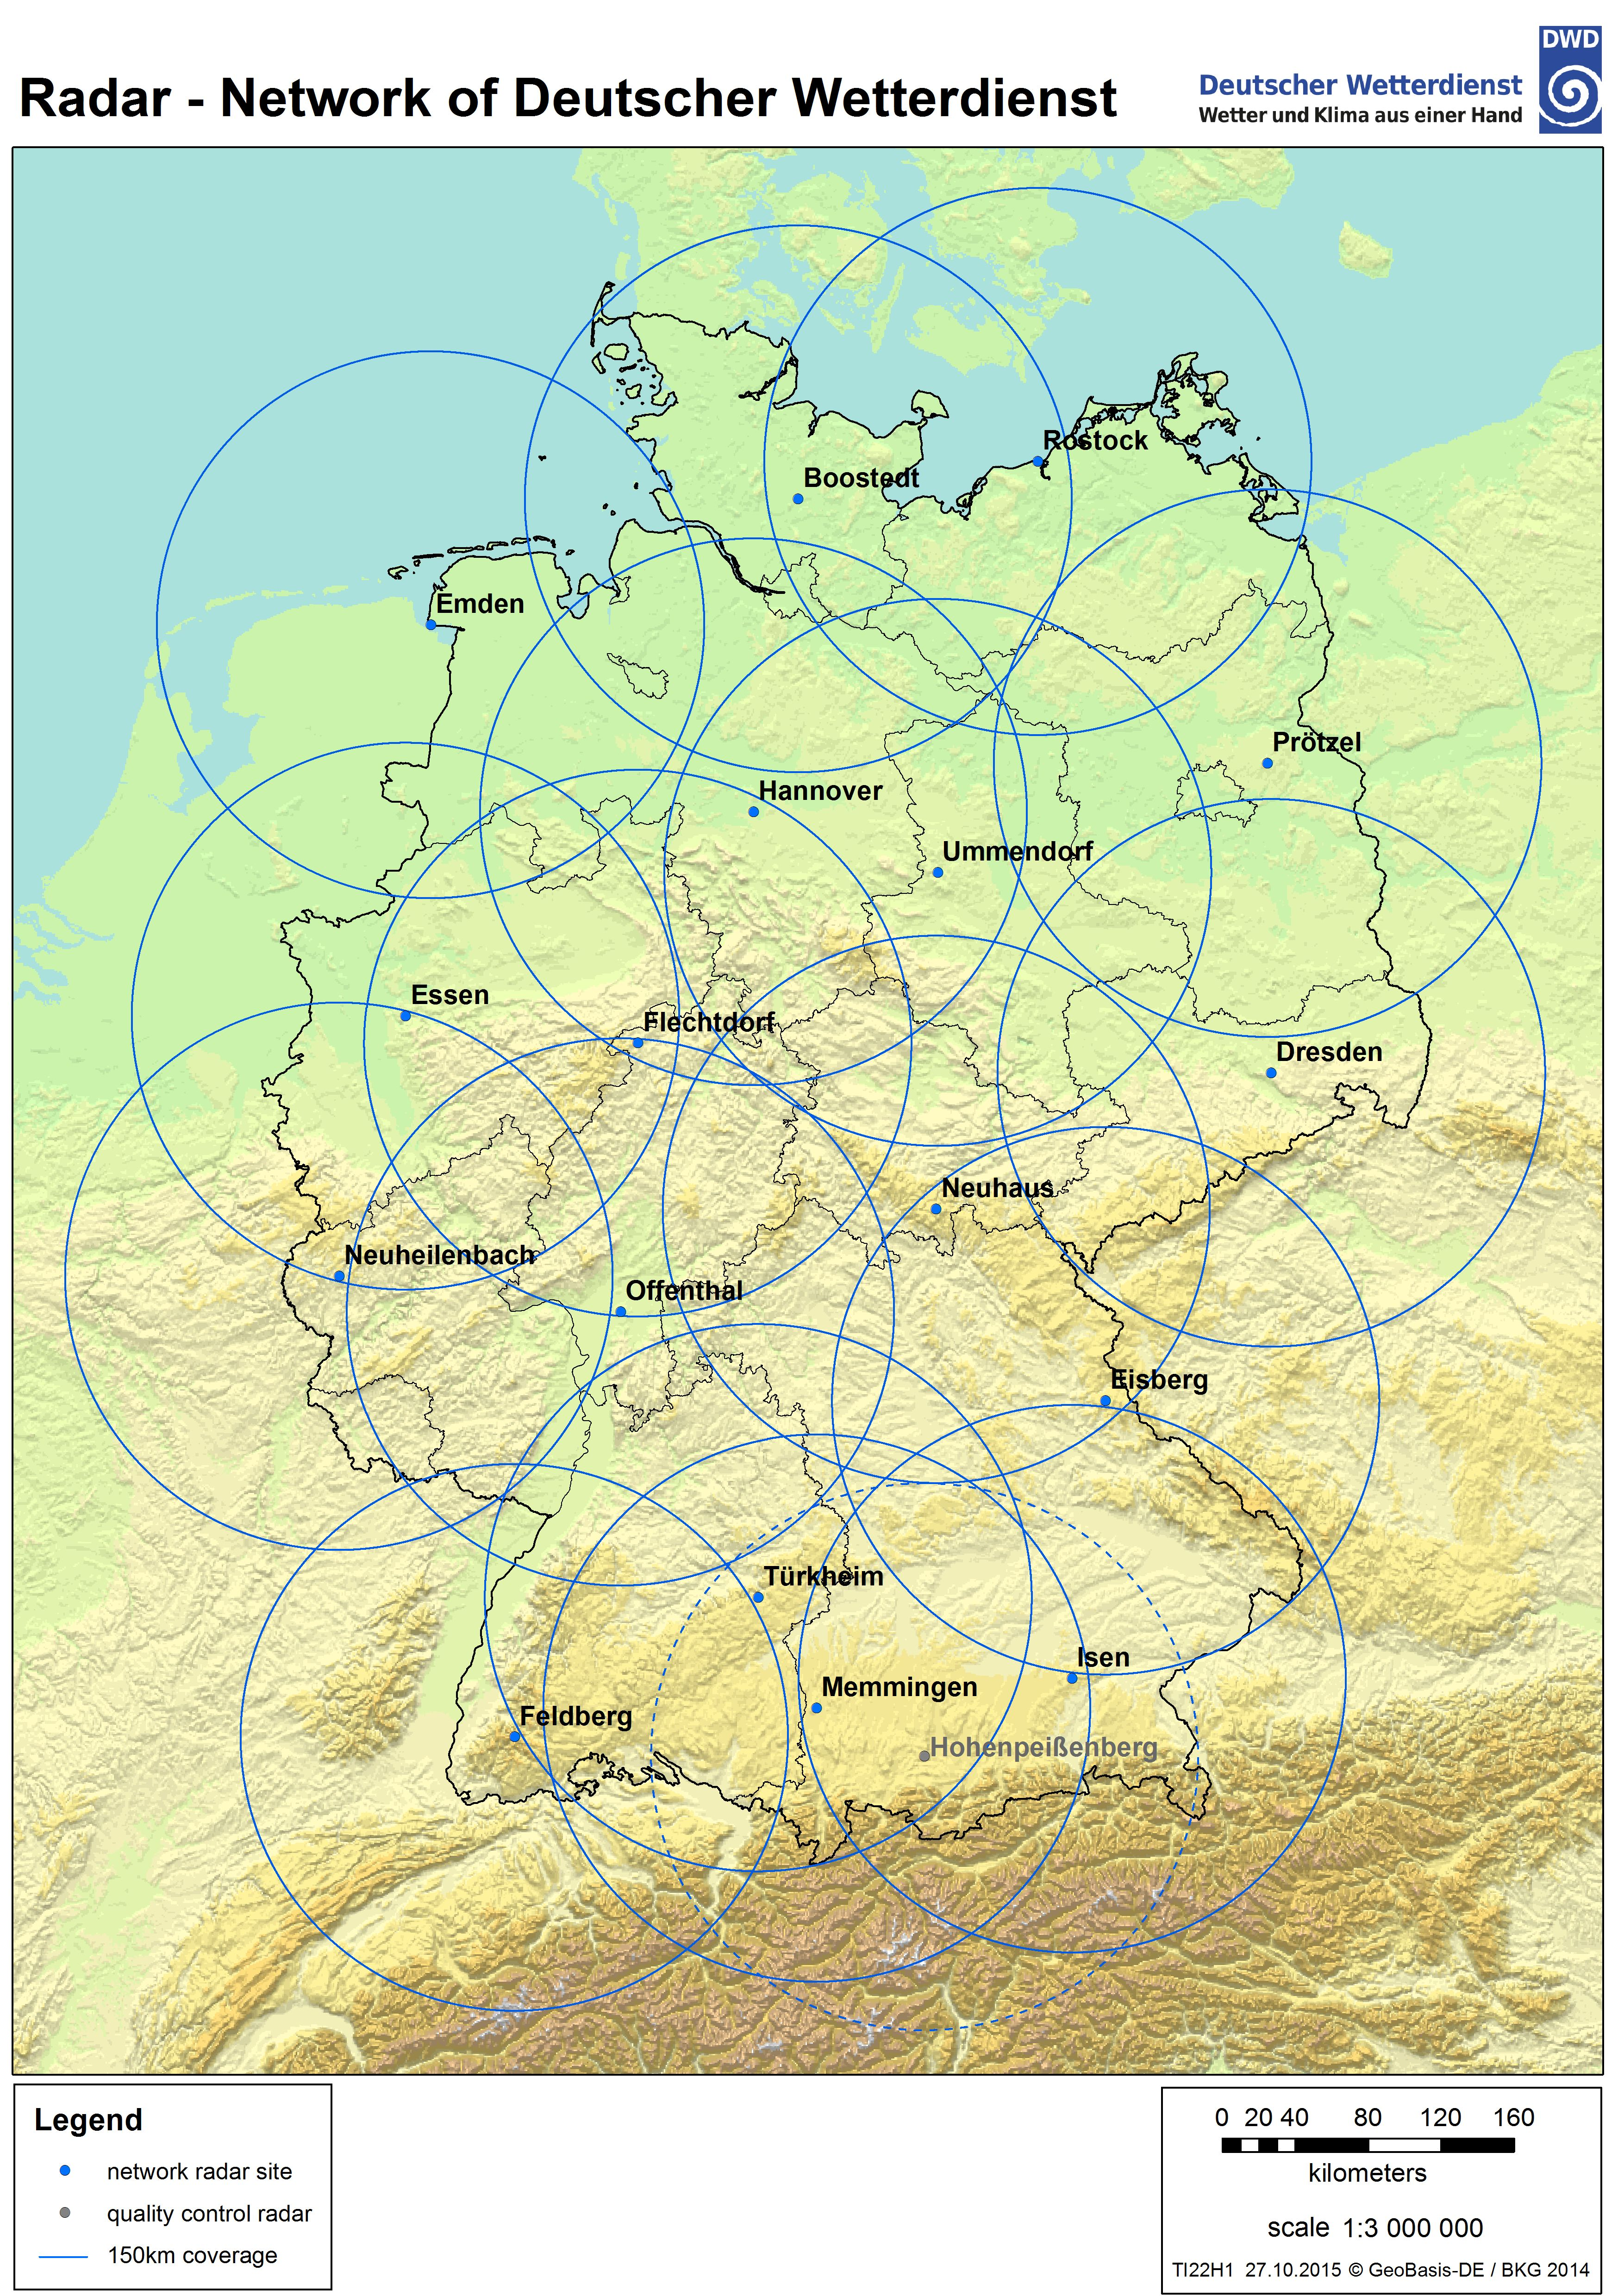
\includegraphics[width=0.9\textwidth]{DWD_RADAR.jpeg}
    \caption{Radar network of the DWD composed of 18 C-Band Radars. 17 of them are operational radars and 1 is a quality assurance radar for testing of new hardware and software (Hohenpeißenberg). The circles depict the 150km range of the radars at their respective centers that are used for the quantitative assessment of precipitation for the RADOLAN products. Figure taken from \citet{DeutscherWetterdienst2022WebsiteDWD}.}
    \label{fig:dwdradar}
\end{figure}

The reflectivity obtained through radar measurements can in theory be converted to a precipitation amount on the ground but in practice the Z-R relationship of \cref{eq:zr} produces deviations from the true value at the ground. For this reason it is useful to utilize the measured precipitation rate at the various rain gauges as true values with which to produce a more value-accurate precipitation distribution. The DWD employs its rain gauges exactly for this purpose. \cref{fig:dwdgauges} shows the location of these gauges in Germany. 

To include the entire catchments covering Germany, rainfall distributions from other radar networks and rain gauges are integrated in the RADOLAN products covering the middle-european area.

\begin{figure}[h!]
    \centering
    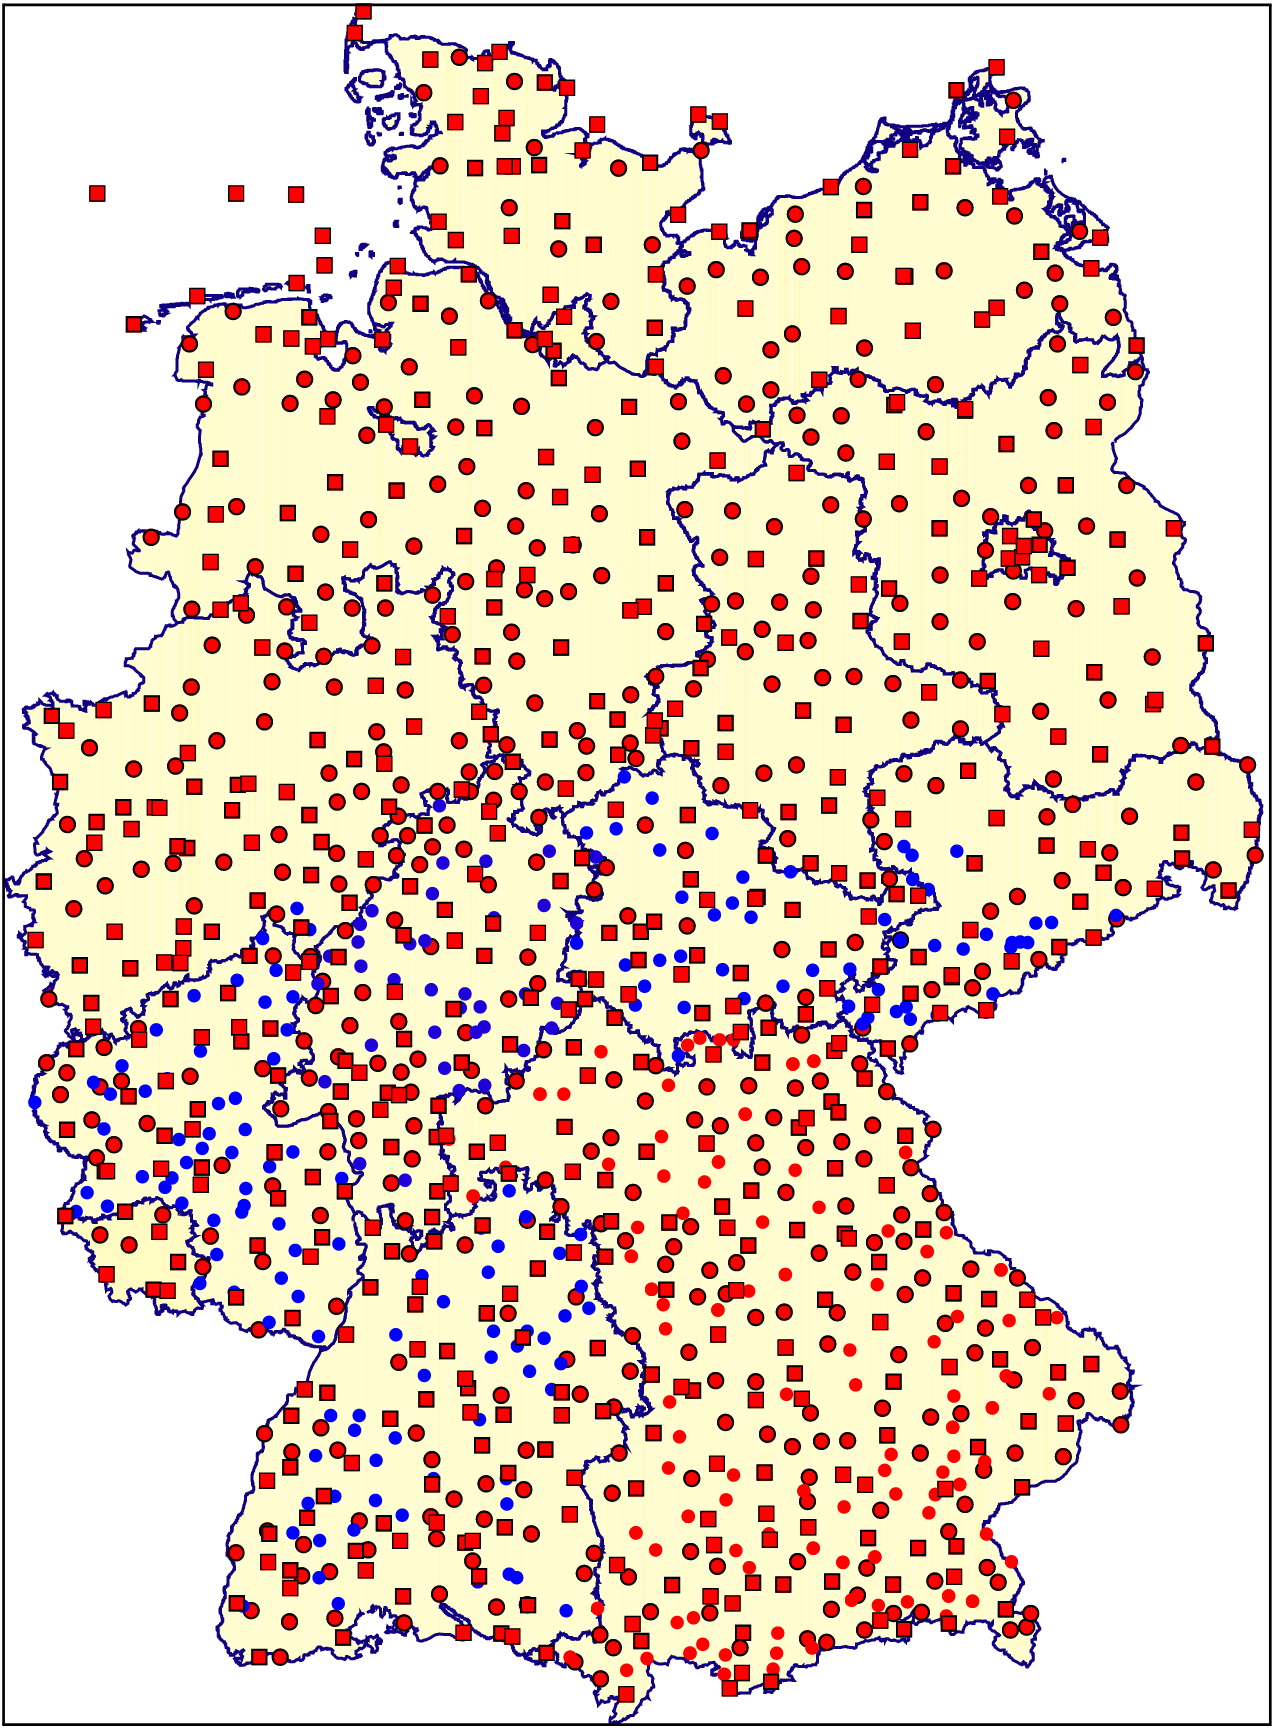
\includegraphics[width=0.9\textwidth]{DWDWeatherStations.png}
    \caption{Regional distribution of the rain gauges of the DWD. \textbf{Squares}: gauges with hourly retrieval; \textbf{circles}: gauges with hourly retrieval in case of precipitation incident (more on when these gauges are activated can be found in \citet{Weigl2004ProjektOmbrometer}) — \textbf{\color{red} Red}: data transmitted through the AMDA III system. (\textbf{without border}: Bavaria); \textbf{\color{blue} blue}: other rain gauges operated by the \textit{Länder}. Image from \citet{Weigl2004ProjektOmbrometer}.}
    \label{fig:dwdgauges}
\end{figure}

\subsubsection{Calibration method}
The RADOLAN calibration routine is very elaborate. I will try to give a very brief overview of its most important components and principles. Please refer to \citet{Weigl2004ProjektOmbrometer} for a complete account and to \citet{Weigl2021RADOLANRoutine} for the subsequent updates.

The routine is applied on a \textit{grid} representing 1km$\times$1km \textit{squares} or \textit{tiles} of data obtained by joining the radar reflectivity maps from the single weather radars. The grid covers the area of Germany and part of its surroundings depending on which Radolan product is considered. The coordinates of the tiles are obtained trhough polar stereographic projection. The projection plane touches the Earth's sphere at 60.0°N. The Cartesian coordinate system has dimensions of 900km$\times$900km and is parallel to the 10.0°E-meridian. The coordinates of the central point of the composite are 9.0°E and 51.0°N. The Earth's sphere is assumed to be regular and with a radius of 6370.04 km . \cref{fig:radolanextension} shows this spatial extension and \cref{fig:grid} shows a depiction of the grid structure where the coordinates of the grid points represent the lower left corner of each tile. 

\begin{figure}[h!]
    \centering
    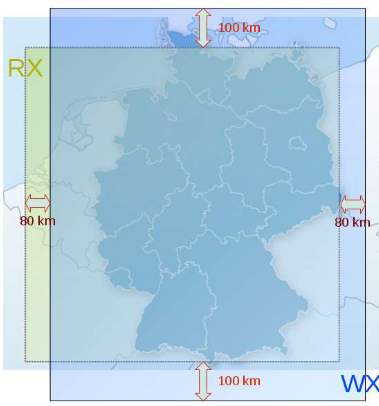
\includegraphics[width=0.6\textwidth]{RadolanExtension.png}
    \caption{Depiction of Germany and the area covered by the RX composite (yellow). The RX composite has the same extension as the RW composite but it represents the uncorrected radar data in RVP6-units. The EX composite (blue) is an expansion of the RX product; it involves a greater area
     taking into account more radars that are not directly operated by the DWD. Figure reprinted from \citet{Weigl2021RADOLAN/RADVOR2.5.3}.}
    \label{fig:radolanextension}
\end{figure}

\begin{figure}[h!]
    \centering
    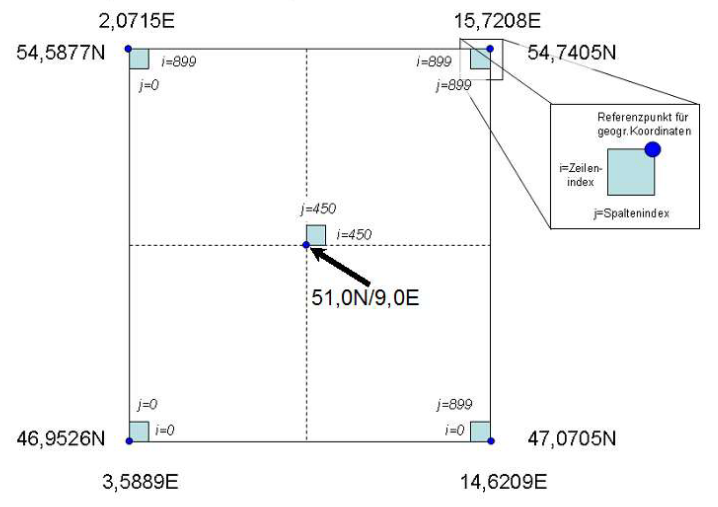
\includegraphics[width=0.8\textwidth]{grid.png}
    \caption{Depiction of the RADOLAN grid and the respective tiles in polar stereographic projection. The arrow points to the center grid point and its respective tile. The indices i and j represent the row and column number of the tile respectively. The blue grid points on the upper left and right corners and on the bottom right corner are shown only to better characterize the extension of the tiles grid. Figure reprinted from \citet{Weigl2021RADOLAN/RADVOR2.5.3}.}
    \label{fig:grid}
\end{figure}
 
The first step in the RADOLAN calibration procedure is a pre-processing step. Here the radar data is compensated for shadowing effects caused by the orography, an empirically derived and more precise reflectivity-rainrate (Z-R) relation is applied following \citet{Weigl2015RadarniederschlagNiederschlages}. Then the various sub-hour radar images are put together, a statistical suppression of clutter is applied by removing hot pixels and substituting them with an interpolated value. Finally in the last part of the pre-processing step the gradients are smoothed down and a pre-calibration with the rain gauges values is put into place \citep{Weigl2004ProjektOmbrometer}.

Subsequently, for the step of the actual calibration, the RADOLAN routine blends three different values for every tile of the composite. The three values are the result of three different calibration methods. 
\begin{enumerate}
    \item The first method consists in finding a multiplicative factor for the radar map. It is based on the assumption that the rain gauges values (RG) and the radar precipitation values (Rad) are related through
    \begin{equation}
        F_{i} = \dfrac{R_i^{\text{RG}}}{R_i^{\text{Rad}}}.
    \end{equation}
    The factors are computed for every relevant i-th rain gauge and corresponding radar composite tile associated to it. The 8 adjacent radar composite tiles are also taken into account. A weighted average takes place to find the interpolation factors for all of the radar tiles. The weights for the average are given by 
    \begin{equation}
        w(d) = \dfrac{\exp({ad})}{1-\exp({ad})}\quad\text{with}\quad a=\dfrac{\ln(0.5)\cdot20}{r_{\text{search}}}
    \end{equation}
    where $d$ is the distance of the tile from a station within a search-radius $r_{\text{search}}$ (typically 40km). This is called the factor-method.
    \item The second method finds a constant to be summed to the radar map. The assumption governing this method is that the relationship between the rain gauges values and the radar precipitation values is of the kind
    \begin{equation}
        D_i = R_i^{\text{RG}} - R_i^{\text{Rad}}.
    \end{equation}
    The procedure to obtain the values of the differences for every tile is the same as for the factor-method. We shall call this the differences-method.
    \item  A third method consisting of the combination of three rainfall distribution maps (1) an interpolated precipitation distribution field on the radar values grid obtained through ordinary kriging using the rain gauges rainfall rates, (2) an interpolated precipitation distribution field on the radar values grid obtained through ordinary kriging using the radar-derived rainfall rates at the points of the rain gauges and (3) the observed radar precipitation distribution. We shall call this the merging-method.
\end{enumerate}
The combination of these three methods follows the equation 
\begin{equation}
    \textbf{R}_{ij} = \dfrac{\textbf{F}_{ij} + \textbf{D}_{ij} + \textbf{M}_{ij}}{w(\textbf{F}_{ij}) + w(\textbf{D}_{ij}) + w(\textbf{M}_{ij})}
\end{equation}
where \textbf{R} is the precipitation matrix and $ij$ are the row and column indices. \textbf{F}, \textbf{D} and \textbf{M} are the results of the factor-method, the differences-method and the Merging-method respectively. The $w$ represent the interpolated weights for the tile {ij}. The weights are derived by comparing the values obtained through the three calibrations method with the true value at a specific subset of the rainfall-affected rain gauges. This subset is called the control rain gauges. The weight for the best calibration method at every control station individually is set to 1 and all the others to 0. An interpolation from these weights to the entire grid of the radar field gives the resulting weights \citep{Weigl2004ProjektOmbrometer}.
\subsubsection{Final product}
The final and best openly available product outputted by the RADOLAN calibration procedure is the so-called RW composite. This composite doesn't include the merging-method of calibration and therefore only employs the factor-method and the differences-method. It is computed every hour and represents the hourly sums of  precipitation as calibrated through the RADOLAN procedure  \citep{Weigl2021RADOLAN/RADVOR2.5.3}. \cref{fig:radolanextension} depicts the extension of the composite over the map of Germany and \cref{fig:radolanexample} shows an example of a single frame of the RW composite. The rainfall rate is given in units of 0.1mm/h for a total of 900km$\times$900km over Germany as previously described.

The RW composite is accessible at \url{https://opendata.dwd.de/climate_environment/CDC/grids_germany/hourly/radolan/}.

\begin{figure}[h!]
    \centering
    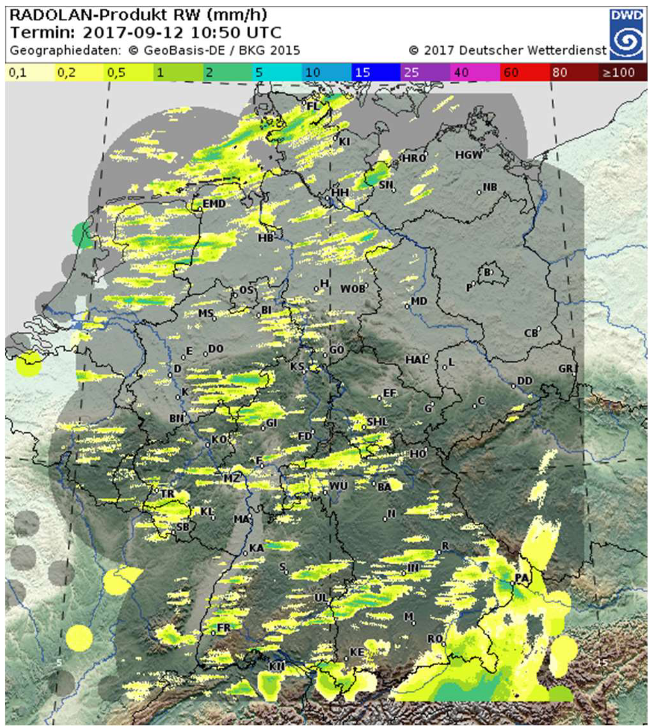
\includegraphics[width=0.6\textwidth]{RADOLAN_EXAMPLE.png}
    \caption{Example of the RW product used in this thesis for the hourly sum at 10:50 UTC of the 12th September 2017. The values are in mm/h and the grey areas are those for which the RW composite is produced. Image reprinted from \citet{Weigl2021RADOLAN/RADVOR2.5.3}.}
    \label{fig:radolanexample}
\end{figure}
\subsection{Dataset Selection - RADNET Dataset} \label{sec:radnet}
I now describe the area of interest and the periods of interest for this project. I also give a short overview of the algorithm used to produce the relevant data for the neural network employed in this thesis. I call this selection the RADNET dataset.
\subsubsection{Area of Interest}
Given that additional measurements errors are introduced by topography, I select a reasonably flat 256km$\times$256km region of the RW product. This part also falls completely inside the area where the RADOLAN routine produces actual values. I therefore select a 256km$\times$256km square with the upper left corner being the nearest grid point to the coordinates 53.6\textdegree N and 8.6\textdegree E. \cref{fig:area_selection} shows the spatial extension of the selection on a map of Germany.

\begin{figure}[!h]
    \centering
    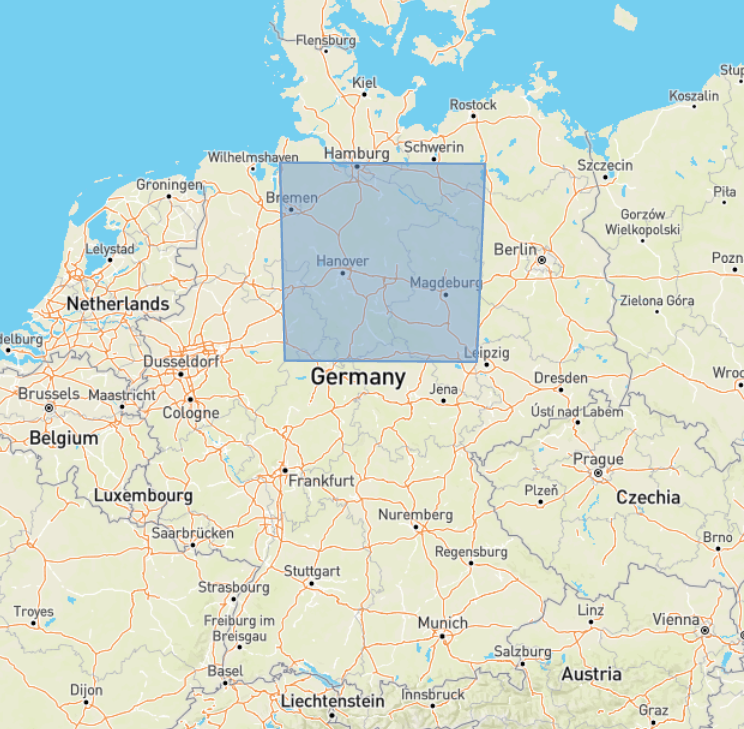
\includegraphics[width=0.7\textwidth]{dataset_selection.png}
    \caption{Area of interest used in this study. The coordinates of the upper left corner are those of the nearest RADOLAN grid-point to 53.6\textdegree N and 8.6\textdegree E. The other corner grid-points are obtained by going 256pixels downwards and 256pixels across. These correspond exactly to 256km southwards and 256km eastwards in the RADOLAN projection plane. The distortion present in this figure is due to the reprojection from the RADOLAN plane to the Mercator projection plane. The figure was created using openstreetmap (\hyperlink{https://www.openstreetmap.org/}{https://www.openstreetmap.org/}) and geojson.io (\hyperlink{https://geojson.io/}{https://geojson.io/}).}
    \label{fig:area_selection}
\end{figure}

\subsubsection{Period of Interest}
In order to not address convective type-precipitations which typically have very short time scales, I decide to concentrate my efforts on the winter months. These go from October through April. I also decide to divide the dataset in three parts, I use the period from 1st October 2005 until 31st December 2017 as my training period. The period from 1st January 2018 until 31st December 2019 is used as the validation set and the period from 1st January 2020 until 31st December 2021 is used as the test set (cf. \cref{sec:datasetdivision}).

\subsubsection{Preprocessing for Neural Network Application} \label{sec:algorithmretrieval}
The purpose of the proposed model is the prediction of a rainfall rate distribution map for the 256km$\times$256km area of interest.

Instead of predicting the specific value of the rainfall rate for a tile of the area of interest, the study after which I based this project predicts whether the rainfall rate falls above a certain threshold \citep{Agrawal2019MachineImages}. This is done for every tile and for each of the 3 thresholds 0.1mm/h, 1mm/h and 2.5mm/h.

To make the prediction more straightforward I address the problem in an equivalent way and decide to predict whether the rainfall rate belongs to one of 4 mutually exclusive classes defined using the same thresholds. These are shown in \cref{tab:prec_classes}.

\begin{table}[!h]
    \centering
    \begin{tabular}{cc}
    \hline
    class & mm/h \\
    \hline
    \hline
   0 & [0, 0.1) \\
   \hline
   0.1 & [0.1, 1.0) \\
   \hline
   1.0 &[1.0, 2.5) \\
   \hline
   2.5 &[2.5, $\infty$) \\
   \hline
    \end{tabular}
    \caption{Precipitation classes used in this study.}
    \label{tab:prec_classes}
\end{table}

The problem formulated in this way is called multi-class segmentation or multi-class classification.

The model, as is expected, receives a series of inputs. The elements given as inputs to the model should contain relevant information for the model to predict the rainfall rate distribution. I decide to call these input elements \textbf{frames}. The frames are composed of 5 channels and have a 256$\times$256 spatial extension. 

The \textbf{first channel} is a 256$\times$256 selection taken from the RADOLAN RW product (see \cref{sec:radolan}). The values of the elements of this channel represent precipitation rate values at a precision of 0.1mm/h as described in the previous section. I call this channel the \textbf{image}.

The \textbf{second} and \textbf{third channels} are respectively the longitude and latitude of the tiles of the image.

The \textbf{fourth} and \textbf{fifth} channels contain information about the time at which the image was produced. The \textbf{fourth channel} is a normalized value for the hour and minute at which the image was taken. Its values range from -1 to 1 where 1 is 00:00 UTC and 1 is 24:00 UTC. The \textbf{fifth channel} contains a normalized day of the year at which the image was produced. It goes from -1 for the 1st of January to 1 for the 31st of December. \citet{Agrawal2019MachineImages} uses only one channel for the time information and employs only the not-normalized time of the day. The choice to normalize the time information is due to the fact that this facilitates a good behaviour of the model. Deciding to add an additional channel for the time information was done because I believe it to be relevant information for the model. If it is not relevant then the model will learn to discard it (see \cref{sec:neuralnet}).

Every input frame is referred to with the same timestamp of the image it contains. \cref{fig:radnetframe} shows a sketch of a frame and its channels.

\begin{figure}[h!]
    \centering
    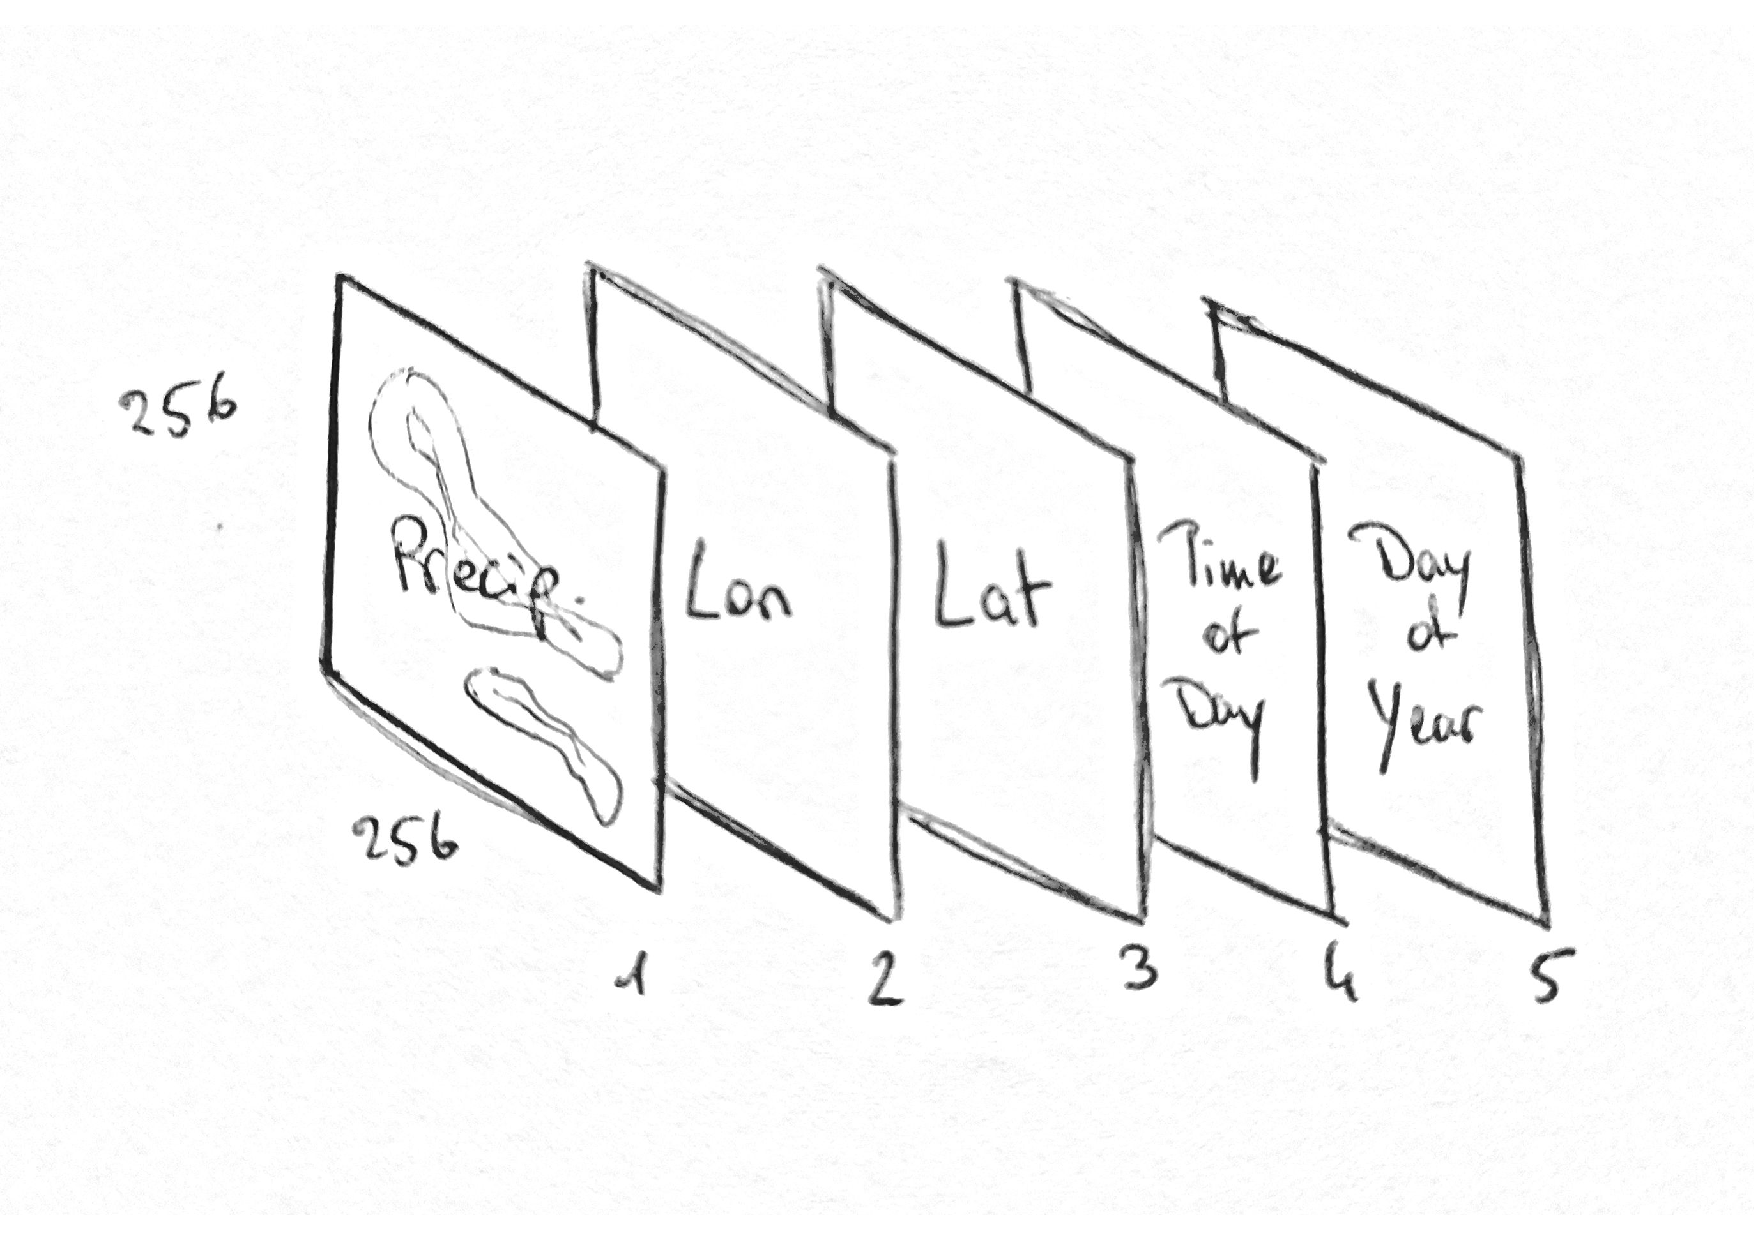
\includegraphics[width=0.7\textwidth]{Frame.pdf}
    \caption{Sketch of a frame. The numbers 1 to 5 represent the channels. 256 stand for the spatial dimensions.}
    \label{fig:radnetframe}
\end{figure}


Finally, considering that a meteorological front has a specific speed when going through the 256km$\times$256km area of interest, I decide to choose the number of frames to give as input to the model by approximating how much time it takes for a front to traverse the selection. Hence, with an average front speed\footnote{Front speeds have very diverse values and depend on different conditions of the system.} of $\approx$10m/s I obtain 6 input frames for the model. Therefore, the model is given 6 input frames taken at 1h intervals from timestamp t until timestamp t+5 and it predicts the class of each tile of the precipitation map for a timestamp t+6. The collection of the 6 input frames together with the ground truth classes precipitation map is called an \textbf{example} (following the general use of the term in the machine learning literature) or \textbf{scene} (to avoid confusion in this project with the common word \textit{example}) and I will refer to it with the timestamp of the first frame. 

I discard from the dataset the scenes with no rain and the scenes where one of the frames has a percentage of tiles of the image with missing precipitation values higher than 10\%. If that percentage is lower I fill the missing values through interpolation. \cref{fig:radnetdatasetexample} shows a single scene and the setup as described above.

\begin{figure}[h!]
    \centering
    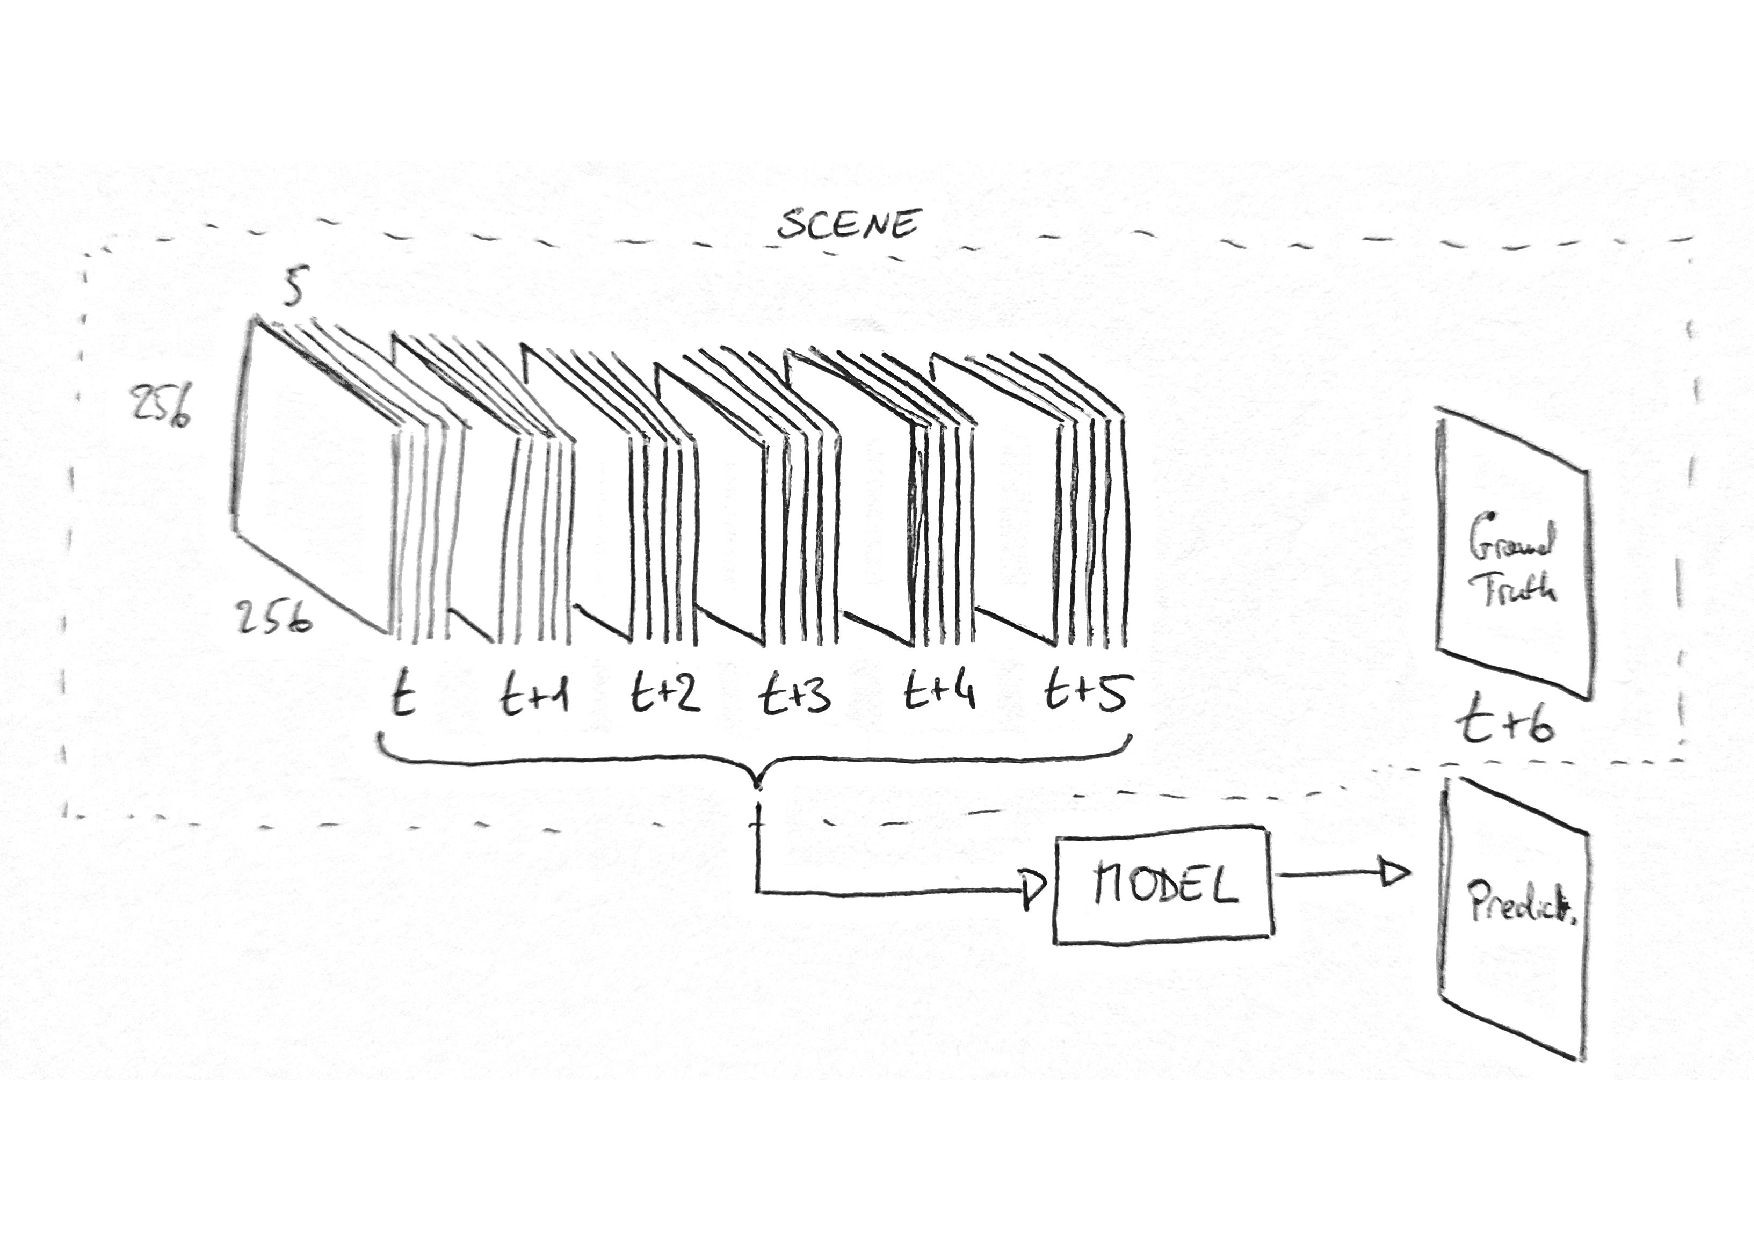
\includegraphics[width=0.85\textwidth]{scene.pdf}
    \caption{Sketch of a scene. The group of 6 frames on the left goes from time t to time t+5. All frames are at 1h distance. These are used by the model to make a prediction that is compared to the ground truth at time t+6. The frames together with the ground truth make a scene.}
    \label{fig:radnetdatasetexample}
\end{figure}


% ==== SECTION 2 ===============================================================
\section{Neural Networks}\label{sec:neuralnet}
In this section I will go through the definition of \textit{machine learning}, its subfield \textit{deep learning} and the rationale behind it (\cref{sec:rationale}). Next, \cref{sec:problemformulation} introduces the concepts of \textit{task}, \textit{performance} and \textit{experience} upon which the machine learning algorithm of this project is built.
\cref{sec:datasetdivision} clarifies the differences between \textit{training}, \textit{validation} and \textit{testing} and how they relate to \textit{hyperparameters}, \cref{sec:nnlay} in turn illustrates the concept of a neural network and its layers. \cref{sec:FullyConnectedLayers} to \cref{sec:softmax} describe all the necessary building blocks of the \textit{neural network architecture} employed for this thesis which is illustrated in \cref{sec:Unet}. The subsequent sections describe the procedures with which the chosen architecture is optimized for the problem addressed in this thesis.

\subsection{Rationale} \label{sec:rationale}
The drive to create machines -- or more specifically algorithms -- that think has been with mankind from the very early days given that it was seen as challenge to recreate, in a way, artificial life.
With the rise of digital computers problems that were difficult for humans but that could be written as simple formal mathematical rules were the first to be addressed. A novice would think that tasks that come natural to us, such as recognizing images or written or spoken words, would also be easy for computers. However, human brains and brains in general are very complex structures tuned and refined by millennia of evolution. It is for this reason that those tasks are some of the most difficult tasks to solve with the help of computers \citep{Goodfellow2016}.

The field responsible for finding a solution to these and more complex yet similar problems goes by the name of \textbf{artificial intelligence} (AI)\footnote{ AI is not to be confused with the more specific \textbf{artificial general intelligence} (AGI) which is what laymen think intuitively of when hearing AI.}.

The very first AI tasks to be solved at the turn of the century were tasks with easy and formal rules; the game of Chess is a notable example. IBM's Deep Blue defeated the world champion Garry Kasparov in one of humanity's most loved strategic games \citep{Campbell2002DeepBlue}. However, every-day life is not made of easy to describe rules like chess; an enormous amount of knowledge that we use is intuitive and subjective, it comes \textit{naturally} to us. In order to solve these same problems a computer needs to be able to capture the same knowledge be it hard-coded or from experience. The first method has been pursued by different projects yet with unsuccessful results hence suggesting that the right path is approaching the quest by building AI systems that form their own intuitive knowledge through extraction from many examples. This ability goes by \textbf{machine learning} (ML) \citep{Goodfellow2016}.
Very simple ML algorithms can solve important problems but need features of the world to be given to them explicitly. For instance, \textbf{logistic regression} can be used to recommend cesarean delivery \citet{Mor-Yosef1990RankingStudy.} yet explicit information about the patient, like the presence of a uterine scar, have to be fed directly. These explicitly coded characteristics of the problem are also called \textbf{features}.
Not every task can be solved through \textbf{feature engineering} and ideally a good AI system should be able to extract those features by itself. \textbf{Deep learning} (DL) solves the problem of extracting high-level abstract features from raw data by expressing them through simpler features and by ignoring variations that don't matter for the task at hand\footnote{Variations that don't matter are for example the time of the day or the color of a car if the task is distinguishing between a car and a motorcycle.} \citep{Goodfellow2016}.

Part of the first ML algorithms that have now become prominent were thought as computational models for biological learning to study ways in which brains in general would learn. This is the reason for which DL, between other names, is also known as \textbf{neural networks} (NNs) or \textbf{artificial neural networks} (ANNs). As the name suggests these are a class of machine learning models that take inspiration from the putative workings of the brain (be it human or of another animal) \citep{Goodfellow2016}. 

Hence, neuroscience gives certain guidelines on which to build upon, the main one being that computational units become intelligent via their interactions; these units have a loose resemblance to neurons. Units are organized in different ways and layers, they take inputs from various other units and produce an output that is gated by an activation function, i.e. the unit forwards the signal only if it exceeds a certain threshold (\cref{sec:ActivationFunctions}) \citep{Goodfellow2016}.

The following sections describe the various parts of a neural network and the algorithm employed in this project.

\subsection{Problem Formulation} \label{sec:problemformulation}
As I stated in the previous section, machine learning algorithms -- and therefore deep learning algorithms -- are programs that learn from experience. In general, quoting \citet{Mitchell1997MachineLearning}: "A computer program is said to learn from experience $E$ with respect to some class of tasks $T$ and performance measure $P$, if its performance in task $T$, as measured by $P$, improves with experience $E$". 

For this project the task $T$ is: given a sequence of images as input I want to predict a subsequent image that appears in the timeseries. This is also called an \textbf{image-to-image problem}. However, for this thesis no prediction of an actual precipitation is made but of categories to which the real values of the predicted pixels would belong to. Hence, this image-to-image problem can be also interpreted as a \textbf{multi-class classification} problem. In fact, for all purposes it is treated as a multi-class classification where the targets are derived by binning the ground truth image. More concisely: for a timestamp $t$ I give as inputs 6 radar-precipitation images embedded into frames from $t$ to $t+5$ (cf. \cref{sec:algorithmretrieval}) to predict the probabilities that a single pixel belongs to one of the precipitation classes of the image at $t+6$. This probability reads, formally
\begin{equation}
    Pr(R_{t+6}|F_t,...,F_{t+5})
\end{equation}
$F_t$ represents a frame at time $t$ and $R$ is the binned rainfall rate target part of the scene associated to the frames $F$. The outputted probability is computed for the 4 mutually exclusive classes for every tile of the 256x256 image.

The performance measures $P$ are the cross-entropy loss, the precision, the recall, the F-measure, the Critical Success Index and the Heidke Skill Score as defined in \cref{sec:metrics}.

The experience $E$ is the RADNET dataset as defined in \cref{sec:radnet}. It is made of scenes which are obtained from the ordered series of radar precipitation images of the RADOLAN dataset.

\subsection{Dataset Division and Hyperparameters} \label{sec:datasetdivision}
In general one is interested to know the goodness of the model on new data. Hence, the performance measures $P$ of the previous sections are normally evaluated on a \textbf{test set}. This subset of the dataset is separate from the data used for training the model which is, in turn, called the \textbf{training set} \citep{Goodfellow2016}.

Machine learning algorithms, in general, posses so-called \textbf{hyperparameters}. These are user-controlled settings that govern the behaviour of the algorithm but are not learned. Nonetheless, algorithms exist to find the optimal hyperparameters set (cf. \cref{sec:hyperparametersearch}). Frequently, parameters that could in theory be optimized on the training set are used as hyperparameters because their optimization would lead to overfitting (see \cref{sec:regularization}). To address this issue, one further breaks down the training set in \textbf{training set} and \textbf{validation set}. Although the nomenclature overlaps with the former interpretation of \textit{training set} when hyperparameters need optimization a \textit{validation set} is needed. This subset of the dataset is used to learn the hyperparameters whilst the \textit{test set} is left completely untouched as it has to serve its role in estimating the generalization error of the model \citep{Goodfellow2016}. A typical ratio of the \textit{training} and the \textit{validation set} is 8:2 but if the dataset is large enough the amount in the \textit{validation set} can be reduced.

\subsection{Neural Networks and Layers} \label{sec:nnlay}
Neural networks are machine learning algorithms that come with different characteristics. In this project a so-called feed-forward neural network is employed in which the information flows only in one direction from the input to the output without coming back to itself with feedback connections.

The structure of a neural network has at its core a fundamental element called unit. Units are vector-to-scalar functions that precisely resemble a neuron's workings because they take inputs from multiple other sources (neurons) and are activated to a different degree based on these weighted inputs \citep{Goodfellow2016}. Multiple neurons acting in concert after the same number of connections from the input are organized in a so-called layer where the input units form the input layer and the output units form the output layer. Additional layers that fall in between the input and the output layers are called hidden layers and their presence renders a neural network deep\footnote{The term deep learning comes, in fact, from Deep Neural Network.} \citep{Goodfellow2016}. The depth of the network is given by the number of layers, while its width corresponds loosely to the number of neurons composing a layer. 

Finally, another parallelism with neuroscience is drawn by using activation functions. These functions are non-linear and differentiable\footnote{Activation functions must only be differentiable in the regions where a gradient for the optimization procedure must be computed. Functions that are normally utilized, such as the Rectified Linear Unit, are not differentiable in some points. This problem is usually of no concern since the probability that the function is evaluated at its non-differentiable point is negligible. Even if this were to happen, the issue could be defined away by simply taking the right derivative.} and represent a threshold that the input signal to a unit has to overcome in order to activate said unit (see \cref{sec:ActivationFunctions}).

Neural networks come in different shapes and employ different layers and components; the specific set of layer choices and other characteristics that make the network are collectively known as the \textbf{architecture} of the network.

The next sections contain the building layers and other architectural characteristics of the neural network used in this thesis up until \cref{sec:Unet} where the architecture is presented to its fullest.

\subsection{Fully Connected Layers}\label{sec:FullyConnectedLayers}
One of the conceptually simplest architecture for a layer in a neural network is built by connecting every unit in a layer to every unit in the layer directly after. Each connection has an associated \textit{weight} and \textit{bias} term that modulate the activation of a single unit based on the signals coming from the units before it \citep{Bishop2006PatternLearning}.

The mathematical expression for a hidden layer would be through a linear combination of its inputs like:
\begin{equation}
    \bm{h} = g \left( \bm{W}^\top \bm{x} + \bm{b} \right)
\label{2equ:1}
\end{equation}
where $\bm{W}$ is the weights Matrix, $\bm{x}$ the input vector, $\bm{b}$ the bias vector and $g$ a differentiable non-linear activation function \citep{Bishop2006PatternLearning, Goodfellow2016}. An example of which is the common function $g(z) = \text{max} \{0, z \}$ also known as Rectified Linear Unit (ReLU). More in \cref{sec:ActivationFunctions}.
A single layer is rarely a good solution and invariably one finds itself stacking multiple of these fully connected layers one after the other \citep{Goodfellow2016}. When multiple layers are employed then the architecture becomes mathematically
\begin{equation}
    \bm{h}^{(1)} = g^{(1)} \left( \bm{W}^{(1)\top} \bm{x} + \bm{b}^{(1)} \right)
\label{equ:FCL1}
\end{equation}
for the first layer. Changing this with the second layer produces
\begin{equation}
    \bm{h}^{(2)} = g^{(2)} \left( \bm{W}^{(2)\top} \bm{h}^{(1)} + \bm{b}^{(2)} \right)
\label{equ:FCL2}
\end{equation}
The subsequent layers are straightforward as is the output layer:
\begin{equation}
    \bm{y} = g^{(n)} \left( \bm{W}^{(n)\top} \bm{h}^{(n-1)} + \bm{b}^{(n)} \right)
\label{equ:FCL3}
\end{equation}
where $n$ is the number of \textit{hidden layers} in the network \citep{Goodfellow2016}.

\subsection{Convolutional Layers} \label{sec:convolutional_layers}

\textbf{Convolutional layers} as an architectural solution are employed when the data has a known grid-like topology as is the case for 1-D grids like time-series or 2-D grids like simple pictures. The intuition underpinning this architecture is that spatially (or temporally) adjacent data-points are highly correlated. A neural network is said to be \textbf{convolutional} if it employs at least one convolutional layer instead of the vanilla matrix multiplication. The name convolution comes from the mathematical operation involved in this type of layers, i.e. \textbf{convolution} \citep{Goodfellow2016}.

Most generally convolution is a mathematical operation on two functions with real-valued argument. It's intuitive interpretation is the weighting average of a function $x$ by a weighting function $w$.
The mathematical definition hereof is the following intergral:
\begin{equation}
    s(t) = \int x(a)w(t-a) \text{d}a \text{.}
\label{2equ:4}
\end{equation}
In order for the output to be a weighted average $w$ needs to be a valid probability density function. However convolution is defined for more general situations and it is a valid operation as long as the integral in \cref{2equ:4} is defined.

Convolution has also its specific mathematical notation:
\begin{equation}
    s(t) = (x \ast w) (t) \text{.}
\label{2equ:5}
\end{equation}

In the case of convolution $x$ is called the \textbf{input}, $w$ the \textbf{kernel} and the output is called the \textbf{feature map}.

The functions in \cref{2equ:4,2equ:5} are continuous and are therefore not a reasonable representation of real-world cases. Real-world data is, unsurprisingly, given in discrete intervals like for instance small timesteps in a time-series or different pixels in an image. One can obtain the discrete version of the convolution operation by employing a discrete sum in place of the integral:

\begin{equation}
    s(t) = (x \ast w) (t) = \sum_{a} x(a) w(t-a) \Delta a \text{.}
\label{2equ:6}
\end{equation}
with $\Delta a$ to be interpreted as a weighting window \citep{Goodfellow2016,Bishop2006PatternLearning}. Both the input and the kernel are normally multidimensional arrays (sometimes also called \textbf{tensors}) and the values of the latter are learned through the learning algorithm. The fact that both have to be stored justifies the reasonable assumption that the functions are 0-valued everywhere on the domain upon which they are defined expect where their values are stored \citep{Goodfellow2016} making the summation finite. 

In real-world DL applications convolution is applied on multi-dimensional tensors and on multiple axis. The simplest case arises for 2-D tensors like images, therefore the 2-dimensional version of \cref{2equ:6} with an image $I$ as input and a 2-dimensional kernel $K$ is

\begin{equation}
    S(i,j) = (I \ast K) (i,j) = \sum_m \sum_n I(m,n)K(i-m,j-n)
\label{2equ:7}
\end{equation}
that, given the commutativity of the convolution operation is equivalent to

\begin{equation}
    S(i,j) = (I \ast K) (i,j) = \sum_m \sum_n I(i-m,i-n)K(m,n)
\label{2equ:8}
\end{equation}
The commutativity of convolution is due to the fact that the kernel is flipped with respect to the input, i.e. when indices increase in one they decrease in the other. Modern libraries, however, implement what is called \textbf{cross-correlation}. This operation is closely related to convolution and in fact it's the same without a kernel-flip \citep{Goodfellow2016}. Its mathematical expression reads
\begin{equation}
    S(i,j) = (K \star I)(i,j) = \sum_m \sum_n I(i+m,j+n)K(m,n)\text{;}
\label{2equ:9}
\end{equation}
Note the star instead of the asterisk for the cross-correlation.
The learning algorithm will learn the values of the appropriate values of the kernel. The kernels resulting from a neural network using cross-correlation will be flipped with respect to the values learned if the implementation is a convolution \citep{Goodfellow2016}. \cref{fig:ConvExample} shows a case of a 2-D discrete convolution without Kernel flipping.

\begin{figure}[h!]
    \centering
    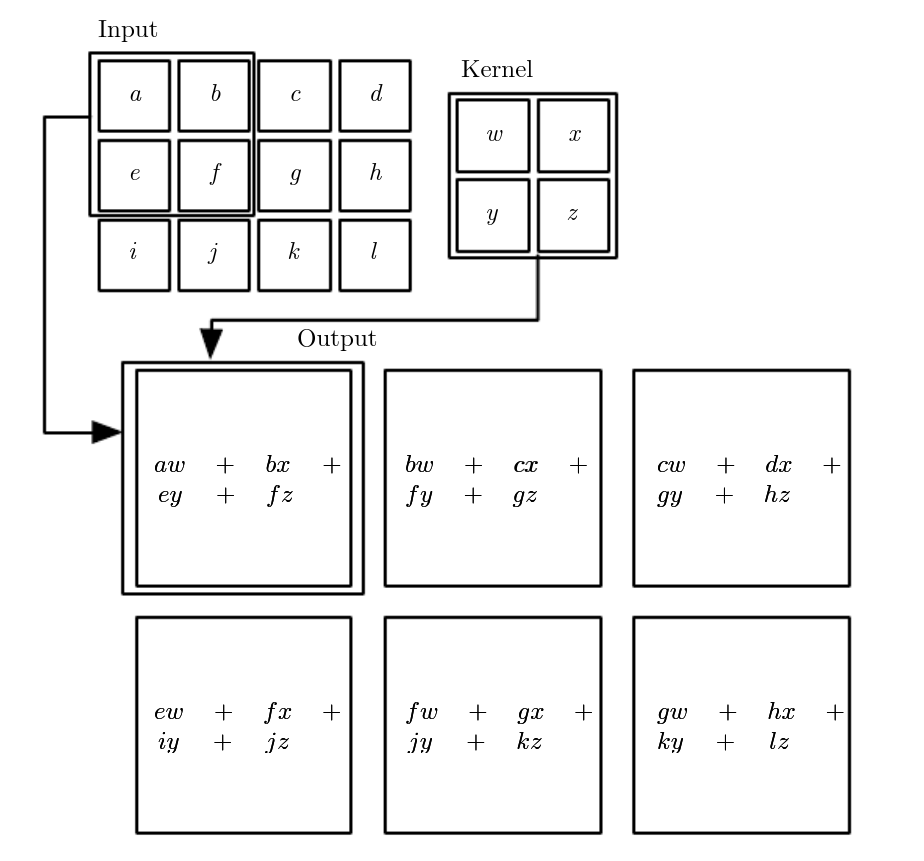
\includegraphics[width=0.8\textwidth]{ConvExample.png}
    \caption{2-D convolution without kernel flipping. The ouptput is restrictied to the places where the kernel fits entirely on the input. The arrows indicate how the indicated output element is obtained from the combination of the selected region of the input tensor and the kernel tensor. Image taken from \citet{Goodfellow2016}.}
    \label{fig:ConvExample}
\end{figure}
Since the appropriate values are the subject of learning by the algorithm, the kernel-flip is irrelevant.

\subsubsection{Advantages}
As it can be intuited from \cref{fig:ConvExample} and as already stated, elements of a tensor that are near each other will influence the corresponding output more than elements that are far from each other. The three main advantages that arise from how convolution is built are sparse interactions, parameter sharing and equivariant representations. 
\subsubsection{Sparse interactions}
Fully connected layers (\cref{sec:FullyConnectedLayers} and \cref{equ:FCL1,equ:FCL2,equ:FCL3}) work through a matrix by matrix multiplication of equal dimensions. Sparse interactions in convolution arise due to the kernels being much smaller than the input matrix, for instance edges in an image of $\sim10^6$ pixels can be easily detected with kernels of $\sim10^2$ pixels \citep{Goodfellow2016}. Smaller kernels mean fewer values to store and increased efficiency\footnote{Considering $m$ inputs and $n$ outputs the simple matrix multiplication has $m\times n$ parameters, $O(m \times n)$ runtime for every example. However, with convolution limiting the number of connections to $k$ for each input, with a much smaller $k$, the number of parameters and the computing time decrease to $k\times n$ and $O(k\times n)$ respectively \citep{Goodfellow2016}.}.

\subsubsection{Parameter sharing}
During a simple matrix multiplication, i.e. the fully connected case, each and every element of the weight matrix is used only once. In contrast, during convolution each parameter of the kernel matrix is used multiple times as the kernel shifts through the input grid. The boundaries of the image are particular in this regard but depend on implementation choices. The runtime is not affected by this property since the number of operations is still $O(k\times n)$ where $k$ is the number of elements in the kernel and $n$ the number of elements of the input. However, the memory footprint is affected substantially given that the number of weights to be stored is now $k$ instead of $m \times n$, which is the dimension of the weight matrix in the fully-connected case \citep{Goodfellow2016}. \cref{fig:ParamSharing} depicts the workings of parameter sharing.

\begin{figure}[!h]
    \centering
    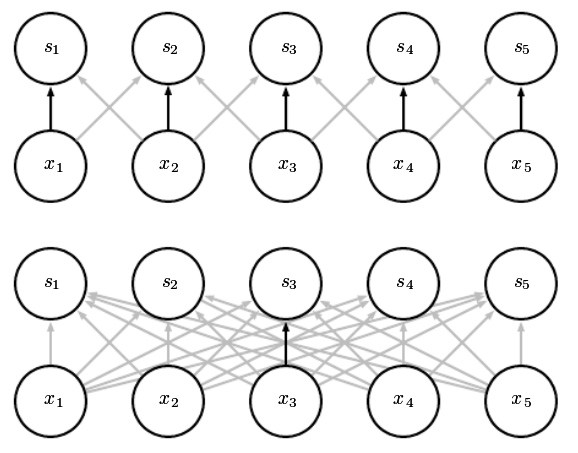
\includegraphics[width=0.6\textwidth]{ParamSharing.png}
    \caption{The top graph is a representation of a convolution with kernel made of $k=3$ elements and an input $\bm{x}$ of $n = 5$ elements. The black arrows are associated with the central element of the kernel. The bottom graph shows the fully-connected case. Here the black arrow represents the central element of the $n \times m = 5 \times 5$ weight matrix $\bm{W}$. Image taken from \citet{Goodfellow2016}.}
    \label{fig:ParamSharing}
\end{figure}

\subsubsection{Equivariance to translation}
The property of equivariance to translation is a consequence of the parameter sharing property: given that a kernel is applied everywhere on the input, the features it detects can be detected anywhere. The term equivariance comes form the mathematical equivariance of a function with respect to another function. A function $f$ is said to be equivariant to a function $g$ if and only if $f(g(x))=g(f(x))$. If $g$ is a function that shifts the input by some distance, we have the case of the equivariance to translation of features to be detected by the kernel $f$ \citep{Goodfellow2016}.

\subsubsection{Indifference to input size}
One last advantage of convolution is its indifference to the input's size. This is a trivial consequence of how kernels are applied to the input. Fully connected layers always need the same input dimensions given that the weight matrix $\bm{W}$ has a fixed size \citep{Goodfellow2016}.

\subsection{Pooling and Unpooling}
Pooling layers are typically employed after a convolution layer and consist of units that substitute an area around a specific location with a summary value such as a maximum (max pooling) or an average (average pooling) \citet{Lecun2015DeepLearning}; these two are the most frequently used pooling functions. Other functions exist\footnote{Some of these functions are $L^2$ norm pooling and distance-weighted average pooling} and are sometimes employed but are not described for simplicity. Given that the averaging and maximum functions are parameter-free no learning occurs in these layers.

Given that a summary statistic is produced over a range of pixels, the pooling areas can be spaced by $k$ pixels instead of just 1. This, in turn, reduces the number of subsequent units by a factor of approximately $k$. An example of this mechanism is shown in \cref{fig:MaxAndAvgPooling}.

\begin{figure}[!h]
    \centering
    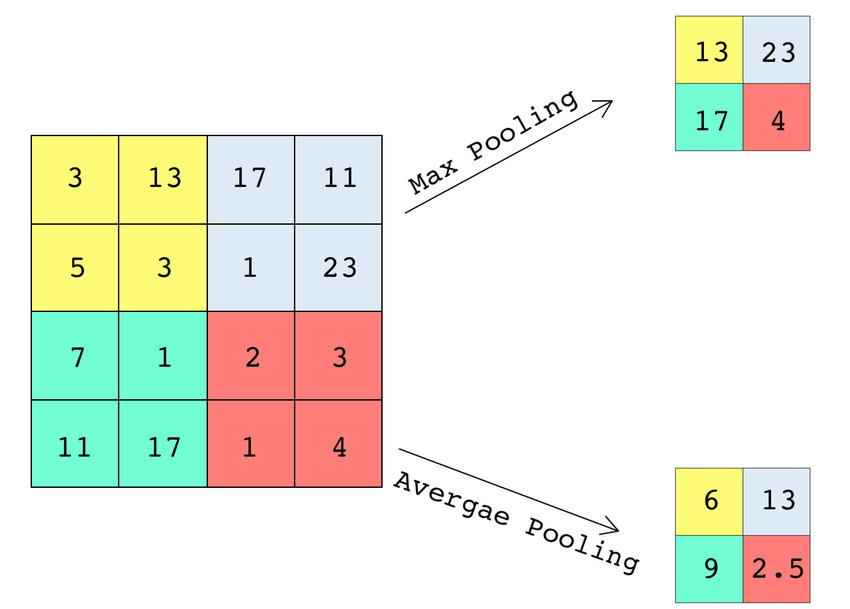
\includegraphics[width=0.6\textwidth]{MaxAndAvgPooling.png}
    \caption{Comparison between average pooling and max pooling of a $4 \times 4$ tensor. The different colors identify the $2\times2$regions over which the average is computed. As is common for pooling the kernel has a stride, i.e. it jumps, by its width instead of going through every pixel. Image taken from \citet{Aljaafari2018IchthyoplanktonLearning}.}
    \label{fig:MaxAndAvgPooling}
\end{figure}

Summary operations make the network approximately invariant to small translations of the input giving more importance to the approximate location and existence of a feature than its precise location in the input grid  \citep{Goodfellow2016}. 

As shown in \cref{fig:MaxAndAvgPooling} the pooling operation with a stride makes the output height and width smaller than the input dimensions. Given that for the architecture employed in this project it's essential for the output to be of the same dimensions as the input (see \cref{sec:Unet}) so-called unpooling layers are used. These layers neither add, nor remove information. When the unpooling operations are done through an \textit{upsampling to the nearest neighbour}, every original pixel is substituted with a new $k\times k$ matrix where every element of the new matrix is equal to the value of the pixel it originated from. 

\subsection{Skip Connections} \label{sec:skip_connections}
Generally more connections are thought to add additional degrees of freedom to a network that give it the possibility to fit much more intricate functions. An hypothesis connected to this seemingly correct assumption is that if errors would arise from adding more layers they would manifest in the form of overfitting. Further, if a layer is not really needed, the network should in theory be able to fit an identity mapping with the non-beneficial layers. However, this has been shown to not be the case in \citet{He2015ConvolutionalCost} and in \citet{Srivastava2015HighwayNetworks} where additional layers lead to degradation not due to overfitting.

As in \citet{He2016DeepRecognition,Srivastava2015HighwayNetworks}, the problem was identified to be a difficulty by the layers to allow a flow of unaltered information to pass through the network. The simplest solution is given by fitting a residual mapping for smaller building blocks of the network instead of the general mapping. This adds no computational cost and is a proven method to address degradation in deeper networks effectively \citep{He2016DeepRecognition}. Formally that would amount to fitting $\mathcal{F}(\bm{x}) = \mathcal{H}(\bm{x}) - \bm{x}$ and obtaining the desired mapping $\mathcal{H}(\bm{x})$ by simple summation $\mathcal{F}(\bm{x}) + \bm{x}$. Hence, in the extreme case, to obtain the identity mapping, the weighted layers would only need to reach $0$. Particular implementations of this fundamental idea were further discussed by \citet{He2016IdentityNetworks}. For a graphical representation see \cref{fig:ResMap}.
\begin{figure}[!h]
    \centering
    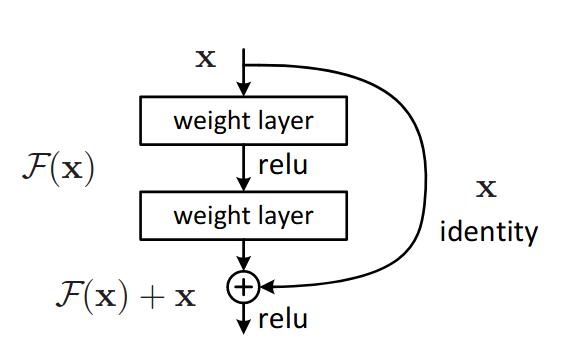
\includegraphics[width=0.6\textwidth]{ResMap.png}
    \caption{The representation of a residual block that fits a desired mapping $\mathcal{H}(\bm{x})$ by making the tunable (weight) layers optimise for the residual $\mathcal{F}(\bm{x}):=\mathcal{H}(\bm{x}) - \bm{x}$. "relu" stands for the correpsonding activation function (cf. \cref{sec:ActivationFunctions}). Example and image taken from \citet{He2016DeepRecognition}.}
    \label{fig:ResMap}
\end{figure}

In the case of U-Nets used in this project (see \cref{sec:Unet} for the implementation), it is good practice to adopt long range skip connections to pass information from a downsampling\footnote{See \cref{sec:Unet}} block to an upsampling\footnote{See \cref{sec:Unet}} block \citep{Drozdzal2016TheSegmentation}. The use of long-range and short-range skip connections for image segmentation was linked to both better performance and faster convergence \citep{Drozdzal2016TheSegmentation}. Both kinds of skip connections can be achieved either by summation -- therefore applying \citet{He2016DeepRecognition} also to long-range skip connections -- or by concatenating the relevant information as in \citet{Shelhamer2017FullySegmentation}.

Further details on the specifics of the implementation in this project will be discussed in \cref{sec:Unet}.

\subsection{Activation Functions} \label{sec:ActivationFunctions}
Activation Functions are an essential building block of neural networks due to the fact that they introduce a necessary \textbf{non-linearity} in the architecture. Were they linear then the neural network would become a combination of only linear components which is equivalent to an architecture without hidden layers \citep{Bishop2006PatternLearning}. There is no canonical choice of activation functions, the only requisites are that they be (1) non-linear and (2) differentiable \citep{Bishop2006PatternLearning,Goodfellow2016}. The appropriate activation function for hidden layers is normally chosen by looking at its properties like ease of computation and lack or presence of saturation. However, for the output layer the choice of the activation function and the corresponding \textit{loss function} are tightly coupled to the problem being solved \citep{Bishop2006PatternLearning}.

Many activation functions have risen in popularity; the three most common for hidden layers to the day of writing according to \citet{PaperswithCode2022AnCode} are the Rectified Linear Unit, the Sigmoid activation function and the Tanh activation function. I will address only a variant of the first one: the Leaky Rectified Linear Unit. As for the activation function for the output unit -- which are sometimes called output functions -- the Softmax activation function is presented.

\subsubsection{Leaky Rectified Linear Unit (LeakyReLU)}

The LeakyReLU activation function has nearly all the properties of the ReLU activation function of which it is a variation \citep{Maas2013RectifierModels}, i.e. no saturation, ease of computation of the gradient and avoidance of the vanishing gradient problem. The only difference is that it is not zero for negative values but linear with a positive -- yet small -- slope. Formally it's defined as,
\begin{equation} \label{eq:LeakyReLU}
    LeakyReLU(x) = \begin{cases} x & x\geq0 \\ a\, x & \text{else} \end{cases} \; \text{with} \; a \in \mathbb{R}^{+}
\end{equation}

The value of $a$ in \cref{eq:LeakyReLU} is traditionally small and in the order of $0.01$ however it can be easily set manually and reach higher values \citep{Xu2015EmpiricalNetwork}. 

The implication of using the LeakyReLU activation function is that there is a gradient, albeit small, for negative values of the input which allows for updating to take place during back-propagation. Computationally this is very efficient compared to alternatives such as \textit{sigmoid} and \textit{tanh}.

\subsubsection{Softmax} \label{sec:softmax}

The Softmax activation function is normally used in the very last layer of a neural network -- also called the output layer -- to address multi-class classification problems. For problems of this sort one needs to produce a vector $\hat{\bm{y}}$ with
\begin{equation}
    \hat{y_i} = P(y=i\mid \bm{x})
\end{equation}
where every element is between 0 and 1 and where the sum of the elements is 1 therefore representing a valid probability distribution. In the practical application of a neural network the last layer before the output layer, being linear, produces an unnormalized log probability\footnote{More on log probabilites and their relevance in \cref{sec:networkoptim}} vector as in
\begin{equation}
    \bm{z} = \bm{W}^\top \bm{h} + \bm{b}
\end{equation}
with
\begin{equation}
    z_i = \log \tilde{P}(y=i \mid \bm{x}).
\end{equation} This corresponds to the unnormalized log probability that the input $\bm{x}$ belongs to the class $i$.

The definition of the Softmax function comes from the need to obtain a normalized probabilty distribution $\hat{\bm{y}}$ by exponentiating and normalizing $\bm{z}$
\begin{equation} \label{eq:softmax}
    \text{softmax}(\bm{z})_i=\dfrac{\exp{z_i}}{\sum_{j=1}^n \exp{z_j}} = \hat{y}_i
\end{equation}
with $i=1,...,n$ \citep{Goodfellow2016}.
This in turn corresponds to the normalized probability that the input $\bm{x}$ belongs to the class $i$.

In the case of image segmentation, as is for this project, for every pixel of the output image there is an associated $\bm{z} \in \mathbb{R}^n$ on which the Softmax function can be applied to categorize every pixel.

% \subsubsection{LogSoftmax}
%
% During the optimization procedure through the Maximum Likelihood Estimation (\cref{sec:Optim}) a differentiation takes place. Given that the natural logarithm is a monotonically increasing function applying it on the Softmax function will not change the location of its maxima. The obtained log-probability is more easily tractable for the purposes of differentiation and it results in the following:
% \begin{equation}
%     \text{log softmax}(\bm{z})_i = z_i - \log \sum_j\exp{z_j}
% \end{equation}
\subsection{U-Net encoder-decoder}\label{sec:Unet}
The task of semantic segmentation, that is the assignment of classes to pixels that belong to the same group, is an ubiquitous problem in the machine learning literature and goes from applictaions such as scene recognition \citep{Badrinarayanan2017SegNet:Segmentation} to identifications of neuronal structures in biomedical images as in \citet{Ronneberger2015U-Net:Segmentation}. The architecture in \citet{Ronneberger2015U-Net:Segmentation} -- a U-Net -- was proposed as an extension of  of the first fully convolutional network architecture for semantic segmentation by \citet{Shelhamer2017FullySegmentation}. 

\subsubsection{Implementation}

An \textit{encoder-decoder} main working is to (1) reduce the spatial dimension of the input and abstract information into a latent space, subsequently (2) return the information to the original format so that it can be interpreted \citep{Goodfellow2016}. This can be done through convolutional layers and, if nothing other than convolution is involved, this architectural choice can be labeled as \textit{fully convolutional encoder-decoders}. A specific implementation thereof is the U-Net architecture \citep{Ronneberger2015U-Net:Segmentation} adopted and re-adapted in this project for the image-to-image problem applied to precipitation nowcasting and inspired from \citet{Agrawal2019MachineImages}. \cref{fig:unet} shows the architecture I employ as described in the following paragraphs.

\subsubsection{Encoder}
The encoder starts with a \textit{basic block} that is composed of a \textit{convolution}, followed by a \textit{batch normalization} layer, a non-linear activation function of the \textit{LeakyReLU} type and an additional \textit{convolution}. 

Subsequently a number of \textit{down sampling blocks} follow. Each block is made of, in order, a \textit{batch normalization}, a \textit{Leaky ReLU}, a \textit{max pooling} layer -- where the actual downsampling occurs -- another \textit{batch normalization} layer, a \textit{Leaky ReLU} and a final \textit{convolution}.

After the \textit{down sampling blocks} of the \textit{encoder} and before the \textit{decoder} I employ an additional \textit{basic block} that serves as a bottleneck.

For the short range skip connections' architecture there are no explicit descriptions in \citet{Agrawal2019MachineImages} other then a reference to \citet{Drozdzal2016TheSegmentation} and \citet{He2016DeepRecognition}. Since both prefer summation rather than concatenation for skip connections, I choose the former. As for the layers in the path followed by the identity mapping, keeping in line with \citet{He2016IdentityNetworks} and \citet{Drozdzal2016TheSegmentation} I use a very simple \textit{average pooling} for the reduction of the spatial resolution and a \textit{1x1 convolution} to adjust the number of feature maps so that a summation is possible after a skip connection. I also add a \textit{batch normalization} layer to mitigate the batch-to-batch variance for small batches.

After every block in the encoder -- and before the summation with the identity mapping -- the intermediate result is stored to be used in a long-range skip connection to the corresponding block in the decoder. \citet{Agrawal2019MachineImages} does not explicitly state whether the long range skip connection is built by taking the output of an encoding block right before the identity mapping is added, however, an image of the architecture in a related blog post\footnote{https://ai.googleblog.com/2020/01/using-machine-learning-to-nowcast.html} made by the authors suggests this to be the case. 

\begin{figure}[h!]
    \centering
    \resizebox{\textwidth}{!}{%

\def\ConvColor{rgb:yellow,5;red,2.5;white,5}
\def\ConvReluColor{rgb:yellow,5;red,5;white,5}
\def\BNColor{rgb:yellow,5;white,5}
\def\ReluColor{rgb:yellow,5;red,15;white,5}
\def\PoolColor{rgb:red,1;black,0.3}
\def\DcnvColor{rgb:blue,5;green,2.5;white,5}
\def\SoftmaxColor{rgb:magenta,5;black,7}
\def\SumColor{rgb:blue,5;green,15}
\def\InputColor{rgb:green,10;black,10;blue,5}
\def\UpsampleColor{rgb:blue,20;green,5;black,5}
\def\SkipColor{rgb:blue,5;red,2.5;white,5}
\def\poolsep{0.2}
\def\horsep{0.7}

\begin{tikzpicture}
\tikzstyle{connection}=[ultra thick,every node/.style={sloped,allow upside down},draw=\edgecolor,opacity=0.6]
%%%%%%%%%%%%%%%%%%%%%%%%%%%%%%%%%%%%%%%%%%%%%%%%%%%%%%%%%%%%%%%%%%%%%%%%%%%%%%%%%%%%%%%%
%% Draw Layer Blocks
%%%%%%%%%%%%%%%%%%%%%%%%%%%%%%%%%%%%%%%%%%%%%%%%%%%%%%%%%%%%%%%%%%%%%%%%%%%%%%%%%%%%%%%%
% input
\pic[shift={(0,0,0)}] at (0,0,0) {Box={name=input,%
        xlabel={{"I","dummy"}},fill=\InputColor,height=40,width=5,depth=40,zlabel=W,caption=Input}};
% basic_block 1
\pic[shift={(\horsep,0,0)}] at (input-east) {Box={name=b1conv1,%
        xlabel={{"I","dummy"}},fill=\ConvColor,height=40,width=5,depth=40}};
\pic[shift={(0,0,0)}] at (b1conv1-east) {Box={name=b1norm,%
        xlabel={{"N","dummy"}},fill=\BNColor,height=40,width=2,depth=40}};
\pic[shift={(0,0,0)}] at (b1norm-east) {Box={name=b1lrelu,%
        xlabel={{"A","dummy"}},fill=\ReluColor,height=40,width=2,depth=40}};
\pic[shift={(0,0,0)}] at (b1lrelu-east) {Box={name=b1conv2,%
        xlabel={{"I","dummy"}},fill=\ConvColor,height=40,width=5,depth=40,zlabel=W/2}};

% downsample_block_1
\pic[shift={(\horsep,0,0)}] at (b1conv2-east) {Box={name=d1norm1,%
        xlabel={{"N","dummy"}},fill=\BNColor,height=40,width=2,depth=40}};
\pic[shift={(0,0,0)}] at (d1norm1-east) {Box={name=d1lrelu1,%
        xlabel={{"A","dummy"}},fill=\ReluColor,height=40,width=2,depth=40}};
\pic[shift={(\poolsep,0,0)}] at (d1lrelu1-east) {Box={name=d1maxpool,%
        xlabel={{"P","dummy"}},fill=\PoolColor,height=30,width=2,depth=30}};
\pic[shift={(\poolsep,0,0)}] at (d1maxpool-east) {Box={name=d1norm2,%
        xlabel={{"N","dummy"}},fill=\BNColor,height=30,width=2,depth=30}};
\pic[shift={(0,0,0)}] at (d1norm2-east) {Box={name=d1lrelu2,%
        xlabel={{"A","dummy"}},fill=\ReluColor,height=30,width=2,depth=30}};
\pic[shift={(0,0,0)}] at (d1lrelu2-east) {Box={name=d1conv,%
        xlabel={{"32","dummy"}},fill=\ConvColor,height=30,width=7.5,depth=30,zlabel=W/4}};
        
% downskip_block_1
%\pic[shift={(0,0,30)}] at (d1norm1-east) {Box={name=ds1conv,%
%        xlabel="B",fill=\ConvColor,height=40,width=7.5,depth=40}};
%\pic[shift={(\poolsep,0,0)}] at (ds1conv-east) {Box={name=ds1avgpool,%
%        xlabel="L",fill=\PoolColor,height=30,width=2,depth=30}};
%\pic[shift={(\poolsep,0,0)}] at (ds1avgpool-east) {Box={name=ds1norm,%
%        xlabel="P",fill=\BNColor,height=30,width=2,depth=30}};
        
% downsample_block_2
\pic[shift={(\horsep,-10.2,0)}] at (d1conv-east) {Box={name=d2norm1,%
        xlabel={{"N","dummy"}},fill=\BNColor,height=30,width=2,depth=30}};
\pic[shift={(0,0,0)}] at (d2norm1-east) {Box={name=d2lrelu1,%
        xlabel={{"A","dummy"}},fill=\ReluColor,height=30,width=2,depth=30}};
\pic[shift={(\poolsep,0,0)}] at (d2lrelu1-east) {Box={name=d2maxpool,%
        xlabel="P",fill=\PoolColor,height=22,width=2,depth=22}};
\pic[shift={(\poolsep,0,0)}] at (d2maxpool-east) {Box={name=d2norm2,%
        xlabel={{"N","dummy"}},fill=\BNColor,height=22,width=2,depth=22}};
\pic[shift={(0,0,0)}] at (d2norm2-east) {Box={name=d2lrelu2,%
        xlabel={{"A","dummy"}},fill=\ReluColor,height=22,width=2,depth=22}};
\pic[shift={(0,0,0)}] at (d2lrelu2-east) {Box={name=d2conv,%
        xlabel={{"64","dummy"}},fill=\ConvColor,height=22,width=12.5,depth=22,zlabel=W/8}};
        
% downskip_block_2
%\pic[shift={(0,0,25.5)}] at (d2norm1-east) {Box={name=ds2conv,%
%        xlabel="B",fill=\ConvColor,height=30,width=12.5,depth=30}};
%\pic[shift={(\poolsep,0,0)}] at (ds2conv-east) {Box={name=ds2avgpool,%
%        xlabel="L",fill=\PoolColor,height=22,width=2,depth=22}};
%\pic[shift={(\poolsep,0,0)}] at (ds2avgpool-east) {Box={name=ds2norm,%
%        xlabel="P",fill=\BNColor,height=22,width=2,depth=22}};
        
% downsample_block_3
\pic[shift={(\horsep,-8.5,0)}] at (d2conv-east) {Box={name=d3norm1,%
        xlabel={{"N","dummy"}},fill=\BNColor,height=22,width=2,depth=22}};
\pic[shift={(0,0,0)}] at (d3norm1-east) {Box={name=d3lrelu1,%
        xlabel={{"A","dummy"}},fill=\ReluColor,height=22,width=2,depth=22}};
\pic[shift={(\poolsep,0,0)}] at (d3lrelu1-east) {Box={name=d3maxpool,%
        xlabel="P",fill=\PoolColor,height=15,width=2,depth=15}};
\pic[shift={(\poolsep,0,0)}] at (d3maxpool-east) {Box={name=d3norm2,%
        xlabel={{"N","dummy"}},fill=\BNColor,height=15,width=2,depth=15}};
\pic[shift={(0,0,0)}] at (d3norm2-east) {Box={name=d3lrelu2,%
        xlabel={{"A","dummy"}},fill=\ReluColor,height=15,width=2,depth=15}};
\pic[shift={(0,0,0)}] at (d3lrelu2-east) {Box={name=d3conv,%
        xlabel={{"128","dummy"}},fill=\ConvColor,height=15,width=17.5,depth=15,zlabel=W/16}};
        
% downskip_block_2
%\pic[shift={(0,0,19.5)}] at (d3norm1-east) {Box={name=ds3conv,%
%        xlabel="B",fill=\ConvColor,height=22,width=17.5,depth=22}};
%\pic[shift={(\poolsep,0,0)}] at (ds3conv-east) {Box={name=ds3avgpool,%
%        xlabel="L",fill=\PoolColor,height=15,width=2,depth=15}};
%\pic[shift={(\poolsep,0,0)}] at (ds3avgpool-east) {Box={name=ds3norm,%
%        xlabel="P",fill=\BNColor,height=15,width=2,depth=15}};
        
% basic_block 2 bottleneck
\pic[shift={(\horsep,-6.5,0)}] at (d3conv-east) {Box={name=b2conv1,%
        xlabel={{"128","dummy"}},fill=\ConvColor,height=15,width=17.5,depth=15}};
\pic[shift={(0,0,0)}] at (b2conv1-east) {Box={name=b2norm,%
        xlabel={{"N","dummy"}},fill=\BNColor,height=15,width=2,depth=15}};
\pic[shift={(0,0,0)}] at (b2norm-east) {Box={name=b2lrelu,%
        xlabel={{"A","dummy"}},fill=\ReluColor,height=15,width=2,depth=15}};
\pic[shift={(0,0,0)}] at (b2lrelu-east) {Box={name=b2conv2,%
        xlabel={{"128","dummy"}},fill=\ConvColor,height=15,width=17.5,depth=15,zlabel=W/16}};
        
% Ball up 1
\pic[shift={(0,6.5,0)}] at (b2conv2-anchor) {Ball={name=sum1,fill=\SkipColor,radius=2.5,logo=$+$}};
        
        
% upsample_block_1
\pic[shift={(\horsep,6.5,0)}] at (b2conv2-east) {Box={name=u1maxpool,%
        xlabel="U",fill=\UpsampleColor,height=22,width=2,depth=22}};
\pic[shift={(\poolsep,0,0)}] at (u1maxpool-east) {Box={name=u1norm1,%
        xlabel={{"N","dummy"}},fill=\BNColor,height=22,width=2,depth=22}};
\pic[shift={(0,0,0)}] at (u1norm1-east) {Box={name=u1lrelu1,%
        xlabel={{"A","dummy"}},fill=\ReluColor,height=22,width=2,depth=22}};
\pic[shift={(0,0,0)}] at (u1lrelu1-east) {Box={name=u1conv1,%
        xlabel={{"64","dummy"}},fill=\ConvColor,height=22,width=12.5,depth=22}};
\pic[shift={(0,0,0)}] at (u1conv1-east) {Box={name=u1norm2,%
        xlabel={{"N","dummy"}},fill=\BNColor,height=22,width=2,depth=22}};
\pic[shift={(0,0,0)}] at (u1norm2-east) {Box={name=u1lrelu2,%
        xlabel={{"A","dummy"}},fill=\ReluColor,height=22,width=2,depth=22}};
\pic[shift={(0,0,0)}] at (u1lrelu2-east) {Box={name=u1conv2,%
        xlabel={{"64","dummy"}},fill=\ConvColor,height=22,width=12.5,depth=22,zlabel=W/8}};
        
% Ball up 2
\pic[shift={(0,8.5,0)}] at (u1conv2-anchor) {Ball={name=sum2,fill=\SkipColor,radius=2.5,logo=$+$}};
        
%% upskip_block_2
%\pic[shift={(0,0,-19.5)}] at (u1maxpool-east) {Box={name=us1upsample,%
%        xlabel="U",fill=\UpsampleColor,height=22,width=2,depth=22}};
%\pic[shift={(\poolsep,0,0)}] at (us1upsample-east) {Box={name=us1conv,%
%        xlabel="C",fill=\ConvColor,height=22,width=12.5,depth=22}};
%\pic[shift={(0,0,0)}] at (us1conv-east) {Box={name=us1norm,%
%        xlabel="B",fill=\BNColor,height=22,width=2,depth=22}};
        
% upsample_block_2
\pic[shift={(\horsep,8.5,0)}] at (u1conv2-east) {Box={name=u2maxpool,%
        xlabel="U",fill=\UpsampleColor,height=30,width=2,depth=30}};
\pic[shift={(\poolsep,0,0)}] at (u2maxpool-east) {Box={name=u2norm1,%
        xlabel={{"N","dummy"}},fill=\BNColor,height=30,width=2,depth=30}};
\pic[shift={(0,0,0)}] at (u2norm1-east) {Box={name=u2lrelu1,%
        xlabel={{"A","dummy"}},fill=\ReluColor,height=30,width=2,depth=30}};
\pic[shift={(0,0,0)}] at (u2lrelu1-east) {Box={name=u2conv1,%
        xlabel={{"32","dummy"}},fill=\ConvColor,height=30,width=7.5,depth=30}};
\pic[shift={(0,0,0)}] at (u2conv1-east) {Box={name=u2norm2,%
        xlabel={{"N","dummy"}},fill=\BNColor,height=30,width=2,depth=30}};
\pic[shift={(0,0,0)}] at (u2norm2-east) {Box={name=u2lrelu2,%
        xlabel={{"A","dummy"}},fill=\ReluColor,height=30,width=2,depth=30}};
\pic[shift={(0,0,0)}] at (u2lrelu2-east) {Box={name=u2conv2,%
        xlabel={{"32","dummy"}},fill=\ConvColor,height=30,width=7.5,depth=30,zlabel=W/4}};
        
% Ball up 3
\pic[shift={(0,10.2,0)}] at (u2conv2-anchor) {Ball={name=sum3,fill=\SkipColor,radius=2.5,logo=$+$}};
        
% upsample_block_3
\pic[shift={(\horsep,10.2,0)}] at (u2conv2-east) {Box={name=u3maxpool,%
        xlabel="U",fill=\UpsampleColor,height=40,width=2,depth=40}};
\pic[shift={(\poolsep,0,0)}] at (u3maxpool-east) {Box={name=u3norm1,%
        xlabel={{"N","dummy"}},fill=\BNColor,height=40,width=2,depth=40}};
\pic[shift={(0,0,0)}] at (u3norm1-east) {Box={name=u3lrelu1,%
        xlabel={{"A","dummy"}},fill=\ReluColor,height=40,width=2,depth=40}};
\pic[shift={(0,0,0)}] at (u3lrelu1-east) {Box={name=u3conv1,%
        xlabel={{"O","dummy"}},fill=\ConvColor,height=40,width=7,depth=40}};
\pic[shift={(0,0,0)}] at (u3conv1-east) {Box={name=u3norm2,%
        xlabel={{"N","dummy"}},fill=\BNColor,height=40,width=2,depth=40}};
\pic[shift={(0,0,0)}] at (u3norm2-east) {Box={name=u3lrelu2,%
        xlabel={{"A","dummy"}},fill=\ReluColor,height=40,width=2,depth=40}};
\pic[shift={(0,0,0)}] at (u3lrelu2-east) {Box={name=u3conv2,%
        xlabel={{"O","dummy"}},fill=\ConvColor,height=40,width=7,depth=40,zlabel=W}};
        
% output
\pic[shift={(\horsep,0,0)}] at (u3conv2-east) {Box={name=output,%
        xlabel={{"O","dummy"}},fill=\SoftmaxColor,height=40,width=7,depth=40,zlabel=W,%
        caption=Output - Softmax}};
        
%paths

\draw[connection](input-east)--node{\midarrow}(b1conv1-west);

\draw[connection](b1conv2-east)--node{\midarrow}(d1norm1-west);

\path (d1conv-east) -- (d2norm1-west|-d1conv-east) coordinate[pos=0.5] (d1-mid) ;
\draw[connection](d1conv-east)--node{\midarrow}(d1-mid)--node{\midarrow}(d2norm1-west-|d1-mid)--node{\midarrow}(d2norm1-west);

\path (d2conv-east) -- (d3norm1-west|-d2conv-east) coordinate[pos=0.5] (d2-mid) ;
\draw[connection](d2conv-east)--node{\midarrow}(d2-mid)--node{\midarrow}(d3norm1-west-|d2-mid)--node{\midarrow}(d3norm1-west);

\path (d3conv-east) -- (b2conv1-west|-d3conv-east) coordinate[pos=0.5] (d3-mid) ;
\draw[connection](d3conv-east)--node{\midarrow}(d3-mid)--node{\midarrow}(b2conv1-west-|d3-mid)--node{\midarrow}(b2conv1-west);

%long skips

\draw[connection](d3conv-east)--node{\midarrow}(sum1-west);
\draw[connection](d2conv-east)--node{\midarrow}(sum2-west);
\draw[connection](d1conv-east)--node{\midarrow}(sum3-west);

%upsampling through sum

\draw[connection](b2conv2-north)--node{\midarrow}(sum1-south);
\draw[connection](u1conv2-north)--node{\midarrow}(sum2-south);
\draw[connection](u2conv2-north)--node{\midarrow}(sum3-south);

\draw[connection](sum1-east)--node{\midarrow}(u1maxpool-west);
\draw[connection](sum2-east)--node{\midarrow}(u2maxpool-west);
\draw[connection](sum3-east)--node{\midarrow}(u3maxpool-west);

%classification
\draw[connection](u3conv2-east)--node{\midarrow}(output-west);
        
\end{tikzpicture}
}
    \caption{Architecture of the U-Net used for this project as in \citep{Agrawal2019MachineImages}. The name comes from the shape it has when displayed in layers. This specific example has the depth hyperparameter -- that controls the number of layers -- set to 3. The left part of the network is called the \textit{encoder} whilst the right part is the \textit{decoder}. The thicker and fainter yellow layers are convolutions with a value standing for the number of feature maps. The number of feature maps is also another hyperparameter, which in this case, is 32. For every layer the number of feature maps doubles. The number of feature maps of the convolutions of the last part of the decoder are denoted with the letter O. In my case they are equal to the number of classes of the output. The bright yellow layers are \textit{batch normalization} layers and are denoted with the letter N. The orange layers stand for the activation function, with the letter A, which in my case are LeakyReLUs. The red layers are \textit{max pooling} operations that reduce the spatial dimensions. The blue layers represent \textit{nearest neighbour upsampling} and invert the pooling process. The arrows represent the flow of information; the ones connecting the blocks from the \textit{encoder} to the sister blocks of the \textit{decoder} are the long skip connections. The skip connections are implemented as summations. The Softmax output layer, depicted in purple, has a number of output channels equal to the number of classes. Short-range skip connections are not depicted for simplicity; they would skip every major block. In this picture every block is separated from other blocks by arrows. \cref{tab:architecture} contains details on the various parameters used for the differente layers, included short-range skip connections.}
    \protect\label{fig:unet}
\end{figure}

\subsubsection{Decoder}
The structure of the \textit{decoder} is similar to the one of the \textit{encoder}. However, an important difference exists: for the purpose of increasing the spatial dimensions it has \textit{upsampling} layers instead of a \textit{max pooling} layers. 

The composition of the \textit{upsampling blocks} is: a \textit{nearest neighbor upsampling} layer, a \textit{batch normalization} layer, a \textit{LeakyReLU} activation layer, a \textit{convolution} and again \textit{batch normalization}, \textit{LeakyReLU} and \textit{convoluion}.

The \textit{short skip connections} are implemented for the \textit{decoder} around every \textit{up-sampling block}. Compared to their counterparts in the encoder section, these skip connections employ the same layers for the same purposes but with \textit{average pooling} substituted by a \textit{nearest neighbor upsampling} layer. \cref{tab:blocks} shows the feature maps for the blocks described in the last two sections.

\begin{table}[!h]
    \centering
    \begin{tabular}{cccc}
    \hline
    \multicolumn{4}{c}{U-Net Building Blocks}\\
    \hline
    \hline
        Layer name & Mathematical operation & Hyperparameter & Value \\
        \hline
         \multirow{5}{*}{Conv2d}& \multirow{5}{*}{Convolution}& kernel size & 3 \\
         & & stride & 1  \\
         & & padding & 1  \\
         & & dilation & 1 \\
         & & \#feature maps & cf \cref{tab:blocks} \\
        \hline
        BatchNorm2d & Batch Normalization & momentum & 0.1 \\
        \hline
        LeakyReLU & Leaky ReLU & negative slope & 0.01\\
        \hline
        \multirow{2}{*}{MaxPool2d} & \multirow{2}{*}{Max Pooling} & kernel size & 2 \\
        & & stride & 2 \\
        \hline
        \multirow{2}{*}{Upsample} & \multirow{2}{*}{Upsampling} & scale factor & 2 \\
        & & mode & nearest neighbor \\
        \hline
        Softmax & Softmax \cref{eq:softmax} & N/A & N/A  \\
        \hline
    \end{tabular}
    \caption{An overview of the different layers that are used as building blocks for the architecture of this project. The name used is the same as the one that appears in the machine learning library \textit{pytorch} in order to favor comparability. An account on how these blocks are put together to form the final architecture is given in both \cref{fig:unet} and \cref{tab:blocks}.}
    \label{tab:architecture}
\end{table}

\begin{table}[!h]
    \centering
    \begin{tabular}{c|ccc}
    \hline
    \multicolumn{4}{c}{Block architectures} \\
    \hline
    \hline
    Block name & Layer name & Input feature maps & Output feature maps \\
    \hline
          \multirow{4}{*}{Basic block} & Conv2d & C & C \\
          & BatchNorm2d & C & C \\
          & LeakyReLU & C & C \\
          & Conv2d & C & C \\
          \hline
         \multirow{6}{*}{Downsampling block}& BatchNorm2d & C & C \\
         & LeakyReLU & C & C \\
         & MaxPool2d & C & C \\
         & BatchNorm2d & C & C \\
         & LeakyReLU & C & C \\
         & Conv2d & C & 2C or IF for first block \\
         \hline
         \multirow{3}{*}{Down skip connection} & 1x1Conv2d & C & 2C \\
         & AvgPool2d & 2C & 2C \\
         & BatchNorm2d & 2C & 2C \\
         \hline
         \multirow{6}{*}{Upsampling block}& Upsample & C & C \\
         & BatchNorm2d & C & C \\
         & LeakyReLU & C & C \\
         & Conv2d & C & C/2 \\
         & BatchNorm2d & C/2 & C/2 \\
         & LeakyReLU & C/2 & C/2 \\
         & Conv2d & C/2 & C/2 or K for last layer \\
         \hline
         \multirow{3}{*}{Up skip connection} & Upsample & C & C \\
         & 1x1Conv2d & C & C/2 \\
         & BatchNorm2d & C/2 & C/2 or K for last layer \\
         \hline
         Final layer & Softmax & K & K \\
         \hline
    \end{tabular}
    \caption{Summary of the number of feature maps associated with each of the layers of the different blocks for the architecture of this project. C is a place holder value for which to compute the other number of feature maps for every layer of the same block. IF stands for the hyperparameter Initial Features which is the number of feature maps of the output of the first downsampling block. K is the number of classes of the task. In this project K=4.}
    \label{tab:blocks}
\end{table}

\subsection{Network Optimization and Training Algorithm} \label{sec:networkoptim}
In this section I will address the principal framework -- called \textbf{maximum likelihood estimator} -- through which a set of neural network parameters $\bm{\theta}$ are found such that they minimize an error measure called the \textit{loss function}, i.e. the deviation of the estimate from the target data-points. I will also discuss how this framework allows us to obtain an appropriate loss function given a certain problem. Moreover, the actual training algorithm and its components as well as the particular implementation used in this project are shown.

\subsubsection{Maximum Likelihood Estimation}
The maximum likelihood principle is a method that allows to determine the appropriate functions that make good estimators for a specific model, i.e. it indicates a clear loss function to minimize \citep{Goodfellow2016}. In simple terms (1) a model must be assumed (2) from that model the likelihood function is derived -- that is the probability that the model results in the given data (3) the likelihood function is maximised (or something equivalent).

Let $\mathbb{Y} = \{\bm{y}^{(1)}, ... , \bm{y}^{(m)}\}$ be the family of all the observed targets and $\mathbb{X} = \{\bm{x}^{(1)}, ... , \bm{x}^{(m)}\}$ representing all the m inputs drawn from the distribution. I call the tuple $(\bm{y}^{(i)}, \bm{x}^{(i)})$ an example. I also define $\bm{Y} = (\bm{y}^{(1)}, ... , \bm{y}^{(m)})$ and $\bm{X} = (\bm{x}^{(1)}, ... , \bm{x}^{(m)})$ to be the input and output tensors respectively.

Let us have a family of model probability distributions with parameters $\bm{\theta}$
\begin{equation}
    p_{\text{model}}(\textbf{y}|\textbf{x}; \bm{\theta})
\end{equation}
for the variables \textbf{y} and \textbf{x} with images being respectively $\mathbb{Y}$ and $\mathbb{X}$. I use this family to estimate the probability distribution
\begin{equation}
    p_{\text{data}}(\textbf{y}|\textbf{x}).
\end{equation}

The likelihood function\footnote{See \citet{Rossi2018MathematicalInference} for a precise account.} is given by 
\begin{equation}
    \mathcal{L}(\bm{\theta}|\textbf{y}; \textbf{x}) = p_{\text{model}}(\textbf{y}|\textbf{x}; \bm{\theta})
\end{equation}
which for the case of i.i.d.\footnote{Independent and identically distributed.} examples means
\begin{equation} \label{eq:likelihoodiid}
    \mathcal{L}(\bm{\theta}|\bm{Y}; \bm{X}) = p_{\text{model}}(\bm{Y}|\bm{X}; \bm{\theta}) = \prod_{i=1}^{m} p_{\text{model}}(\bm{y}^{(i)}|\bm{x}^{(i)}; \bm{\theta}).
\end{equation}

one then has the definition of \textbf{maximum likelihood estimator} for $\bm{\theta}$ as in \citet{Goodfellow2016}. It reads
\begin{equation}
    \bm{\theta}_{\text{ML}} = \argmax_{\bm{\theta}} p_{\text{model}}(\bm{Y}|\bm{X}; \bm{\theta})
\end{equation}
and by assuming that the examples are i.i.d. one can rewrite this expression as
\begin{equation} \label{eq:mleprod}
    \bm{\theta}_{\text{ML}} = \argmax_{\bm{\theta}} \prod_{i=1}^m p_{\text{model}}(\bm{y}^{(i)}|\bm{x}^{(i)}; \bm{\theta}).
\end{equation}

However, \cref{eq:mleprod} has a clear issue when implemented numerically since probabilities have values $0\leq p_{\text{model}}(\bm{y}^{(i)}|\bm{x}^{(i)}; \bm{\theta}) \leq 1$ and their product can become really small causing numerical underflow. To facilitate the numerical optimization one can use a monotonically increasing function and obtain an equivalent numerical optimization problem. The function commonly used is the logarithm that converts a product into a sum. One obtains log likelihoods instead of likelihoods:
\begin{equation} \label{eq:maxlikelihood}
    \bm{\theta}_{\text{ML}} = \argmax_{\bm{\theta}} \sum_{i=1}^m \log p_{\text{model}}(\bm{y}^{(i)}|\bm{x}^{(i)}; \bm{\theta}).
\end{equation}
Conveniently a sum of logarithms for small $p_{\text{model}}$ will reach negative values instead of the very small but positive values had it been a product \citep{Goodfellow2016}. \\

I will now show how maximizing the likelihood is equivalent to a minimization of the so-called cross-entropy.
\subsubsection{Cross-Entropy}
This subsection is written after \citet{Cover2006ElementsTheory} -- where a more precise account on information-theory can be found --  and \citet{Goodfellow2016}.

One first defines a measure of the uncertainty of a random variable, this measure is normally called \textbf{Shannon entropy}. For a discrete random variable x with probability mass function $p(x)$ it reads as follows
\begin{equation}
    H(\text{x}) = - \sum_x p(x) \log p(x)
\end{equation}
which can be interpeted as the expected value of a random variable $\log \frac{1}{p(\text{x})}$ with x having a probability mass function $p(x)$. One obtains
\begin{equation} \label{eq:entropy}
    H(\text{x}) = \mathbb{E}_{\text{x}\sim p}\left[\dfrac{1}{\log p(\text x)}\right] = -\mathbb{E}_{\text{x}\sim p}[\log p(\text x)],
\end{equation}
which is also sometimes written as $H(p)$.

As stated, the entropy of a random variable measures the amount of information needed to describe the random variable. A related concept is the relative entropy, which is a measure of the dissimilarity between two probability distributions. 

Let $p(x)$ and $q(x)$ be two probability mass functions. Their relative entropy or Kullback-Leibler divergence is defined as

\begin{equation} 
    D_{\text{KL}}(p||q) = \sum_x p(x) \log \dfrac{p(x)}{q(x)}
\end{equation}
which, in a similar fashion to entropy it can be interpreted as the expected value of a random variable equal to $\log \frac{p(\text x)}{q(\text x)}$ where x follows a distribution $p$. This means
\begin{equation} \label{eq:dkl}
   D_{\text{KL}}(p||q) = \mathbb{E}_{\text x\sim p} \left[\log \dfrac{p(\text x)}{q(\text x)}\right] = \mathbb{E}_{\text x\sim p}[\log p(\text x) - \log q(\text x)].
\end{equation}
The KL divergence, although sometimes referred to as a \textit{distance} between two distributions, is not really a distance because it's not symmetric, i.e. $D_{\text{KL}}(p||q) \neq D_{\text{KL}}(q||p)$.

The cross-entropy between two distributions $p$ and $q$ is similar to the KL divergence and is defined as
\begin{equation}  \label{eq:crossentropy}
    H(p,q) = H(p) + D_{\text{KL}}(p||q)
\end{equation}
hence, by virtue of \cref{eq:dkl,eq:entropy}
\begin{equation}
    H(p,q) = -\mathbb{E}_{\text x\sim p}[\log q(\text x)]
\end{equation}
which is equivalent to
\begin{equation} \label{eq:crossentropysum}
    H(p,q) = - \sum_x p(x) \log q(x).
\end{equation}
It's clear from \cref{eq:crossentropy} that minimizing the cross-entropy with respect to $q$ is equal to minimizing $D_{\text{KL}}(p||q)$ with respect to $q$.

Let $p(\bm{x})$ be the empirical distribution $\hat{p}_{\text data}(\bm{x})$ as implied by the dataset and defined as the relative frequency of $\bm{x}$ in a set of $n$ samples of the type $\bm{x}^{(i)}$, that is:
\begin{equation}
    \hat{p}_{\text{data}}(\bm{x}) = \dfrac{1}{n} \sum_{i=1}^{n} \delta_{\bm{x}}(\bm{x}^{(i)})
\end{equation}
and let $q(\bm{x})$ be the model distribution $p_{\text{model}}(\bm{x};\bm{\theta})$.
By inserting the newly defined $p$ and $q$ in \cref{eq:crossentropysum} one obtains
\begin{align}
    H(\hat{p}_{\text data}(\bm{x}), p_{\text{model}}(\bm{x};\bm{\theta})) & =  - \sum_x \hat{p}_{\text data}(\bm{x}) \log p_{\text{model}}(\bm{x};\bm{\theta}) \\ & = - \dfrac{1}{n} \sum_{i=1}^{n} \log p_{\text{model}}(\bm{x}^{(i)};\bm{\theta})
\end{align}
which applied to the supervised-learning case and compared to \cref{eq:maxlikelihood} and allows us to conclude that the maximization of the likelihood is equivalent to the minimization of the cross-entropy between the model distribution and the empirical distribution. This reads
\begin{align}
    \bm{\theta}_{\text{ML}} & = \argmax_{\bm{\theta}} \sum_{i=1}^m \log p_{\text{model}}(\bm{y}^{(i)}|\bm{x}^{(i)}; \bm{\theta}) \\
    & = \argmin_{\bm{\theta}} - \dfrac{1}{m} \sum_{i=1}^m \log p_{\text{model}}(\bm{y}^{(i)}|\bm{x}^{(i)}; \bm{\theta}) \\
    & = \argmin_{\bm{\theta}} H(\hat{p}_{\text data}(\bm{x}), p_{\text{model}}(\bm{x};\bm{\theta})).
\end{align}

Since in general one wants to minimize a so-called \textbf{cost function}, the maximum-likelihood principle gives us a natural cost function for a certain model distribution. This cost function is sometimes referred with the symbol $J(\bm{\theta})$ and is simply the negative of the log-likelihood of the model, equivalent to the cross-entropy. \\

In the next section I will derive the expression for the log-likelihood for the multi-class classification problem.
\subsubsection{Maximum likelihood for the multi-class classification problem}
The maximum likelihood principle can be easily applied to the multi-class classification problem. For this family of problems one main assumption is needed: that the target vector $\bm{y}_i \in \mathbb{R}^K$ for the i-th example follows a categorical distribution with K-classes that are mutually exclusive. The distribution has the following form
\begin{equation}
    p(\bm{y}_i| \bm{z}_i, \bm{\theta}) = \prod_{c=1}^{K} \pi(\textbf{y}_i = \bm{1}_c | \bm{z}_i, \bm{\theta})^{y_{ic}} = \prod_{c=1}^K \pi_{ic}^{y_{ic} }
\end{equation}
with the single modelled probabilities $\pi_{ic} = \pi(\textbf{y}_i=\bm{1}_c|\bm{z}_i, \bm{\theta})$ that, given the i-th feature vector $\bm{z}_i$ and the model parameters $\bm{\theta}$, the i-th element belongs to class $c \in \{1,...,K\}$ as encoded in a one-hot vector $\bm{1}_c$ -- a vector with one element equal to $1$ and all other elements equal to $0$ -- of length $K$ \citep{Goodfellow2016,Bishop2006PatternLearning}. Also, we have the target vector $\bm{y}_i = (y_{i1},..., y_{ic},...,y_{iK})$ being too a one-hot vector with $1$ in the position $c$ corresponding to the actual class of the example. 

The likelihood for a categorical distribution with m examples, following \cref{eq:likelihoodiid}, reads
\begin{equation}
    \mathcal{L}(\bm{\theta}|\bm{Y}; \bm{X}) = \prod_{i=1}^{m} p_{\text{model}}(\bm{y}^{(i)}|\bm{x}^{(i)}; \bm{\theta}) = \prod_{i=1}^{m} \prod_{c=1}^K \pi_{ic}^{y_{ic}}
\end{equation}
and since on wants to minimize a cost function $J(\bm{\theta})$, that is defined as the negative of the log-likelihood according to the maximum likelihood principle, it follows
\begin{equation} \label{eq:crossentropyloss}
    J(\bm{\theta}|\bm{Y}, {\bm{Z}}) = - \log \mathcal{L}(\bm{\theta}|\bm{Y}, {\bm{Z}}) = - \sum_{i=1}^m \sum_{c=1}^K y_{ic} \log \pi_{ic}
\end{equation}
with the feature tensor $\bm{Z} = (\bm{z}^{(1)}, ..., \bm{z}^{(m)})$ and the target tensor $\bm{Y} = (\bm{y}^{(1)}, ..., \bm{y}^{(m)})$
This loss function is also called \textit{categorical cross-entropy loss}. Some authors refer to it as simple \textit{cross-entropy} or \textit{cross-entropy loss} although this is a misnomer since a loss composed of negative log likelihoods is always a \textit{cross-entropy} between the empirical target distribution of the training dataset and the model probability distribution \citep{Goodfellow2016}. 

The \textit{categorical cross-entropy loss} can also be implemented with weights to compensate for class-imbalances in the data-set. The weights are inserted by multiplying every term of the sum in \cref{eq:crossentropyloss} by a weight $w_c$ dependent on the class $c$. 

Depending on the machine learning library the loss of \cref{eq:crossentropyloss} is sometimes implemented with a normalizing factor of $\frac{1}{m}$ to obtain a mean. In the case that weights were used the normalizing factor is the inverse of all weights employed in the computation of the loss. That is,
\begin{equation}
    \dfrac{1}{\sum_{i=1}^{m} \sum_{c=1}^K y_c^{(i)} w_c}.
\end{equation}

However, a multiplication of the loss function by a scalar doesn't affect the optimization problem which remains
\begin{equation} \label{eq:mlpcostfunction}
    \bm{\theta}_{\text{ML}} = \argmin_{\bm{\theta}} J(\bm{\theta}|\bm{Y}, {\bm{Z}})
\end{equation}

The distribution commonly used for the last layer in the case of multi-class classification is the softmax function \citep{Goodfellow2016}, which after \cref{eq:softmax} means
\begin{equation}
    \pi_{c}^{(i)} = \pi(\textbf{y}^{(i)} = \bm{1}_c | \bm{z}^{(i)}; \bm{\theta}) = \text{softmax}(\bm{z}^{(i)}(\bm{\theta}))_c = \dfrac{\exp{z_c^{(i)}}}{\sum_{j=1}^K \exp{z_j^{(i)}}} = \hat{y}_c^{(i)}.
\end{equation}
The tensor $\bm{Z}$ is none other than the a tensor of the feature maps of the second-last layer of my actual model. The optimization algorithm, which updates the parameters -- weights and biases -- $\bm{\theta}$ that give rise to the loss, does so by updating them necessarily into the non-linear model that outputs $\bm{Z}$. The mechanism through which this happens is called \textbf{error back-propagation} and is addressed further along this section.
\subsubsection{Gradient-Based Optimization}
As shown in the previous section there is a natural loss function given the particular properties of the task of multi-class classification \cref{eq:crossentropyloss} and the resulting optimization problem in \cref{eq:mlpcostfunction} thanks to the maximum-likelihood principle. The objective is then to find a vector of parameters $\bm{\theta}$ that minimizes the loss function $J(\bm{\theta}|\bm{Y},{Z})$.

Recalling simple calculus we know that when the gradient of a function $\nabla_{\bm{x}} f(\bm{x})$ vanishes then the function has reached a stationary point, also called a critical point and it is either a maximum, a saddle point or a minimum. What distingushes them is the second derivative. If a maximum is also the highest value the function reaches in its entire domain it is called a global maximum, viceversa for a minimum. In theory one needs to find a solution for the equation
\begin{equation} \label{eq:nabla0}
    0 = \nabla_{\bm{\theta}}J(\bm{\theta}|\bm{Y},\bm{Z})
\end{equation}
however this is analytically intractable \citep{Bishop2006PatternLearning}. The main solution to find a point that satisfies \cref{eq:nabla0} is through a gradient-based optimization algorithm \citep{Goodfellow2016,Bishop2006PatternLearning}. The intuition behind this simple algorithm is that the gradient of a function points towards the direction where the function increases the fastest. By using this information one can step-wise evaluate the gradient of the loss for a certain set of parameters $\bm{\theta}$ and then update the vector according to the newly computed gradient and opposite to it. The $\tau\text{-th}$ step of the algorithm looks like
\begin{equation} \label{eq:gradientoptim}
    \bm{\theta}^{(\tau)} = \bm{\theta}^{(\tau - 1)} - \gamma \nabla_{\bm{\theta}} J(\bm{\theta}|\bm{Y},\bm{Z}) \bigg|_{\bm{\theta} = \bm{\theta}^{(\tau)}}.
\end{equation}
The value $\gamma$ is a hyperparameter -- also called learning rate -- and is normally assumed to be small \citep{Goodfellow2016,Bishop2006PatternLearning}.\\

For the computation of the actual gradient over the dataset one would, in theory, need to evaluate the model for every example of the dataset. This is very expensive especially in terms of memory usage and it is commonly preferred to use only a subset of examples for every step. Further, it is normal to expect that the training set has some redundancy in it in the form of examples that contain very similar information and therefore contribute in the same way to the gradient. Finally, there are less then linear returns that come by just adding examples for the estimate of $\nabla_{\bm{\theta}} J(\bm{\theta})$ so that the benefit of using 100 times more memory and computation yields an accuracy that is less than 100 times higher \citep{Goodfellow2016}.

Optimization algorithms can either use the entire training set, a single example or a number of examples that are less than the whole training set. These three cases are called, in order, \textbf{batch} or \textbf{deterministic}, \textbf{stochastic} or \textbf{online}, \textbf{minibatch} or \textbf{(minibatch) stochastic}. The number of examples for every step is also called the \textit{batch size} and is another hyperparameter. It's clear how the \textbf{deterministic} approach and the \textbf{online} approach are just special cases of the more general \textbf{minibatch}: in the first one the \textit{batch size} is simply equal to the length of the dataset whilst in the second case the same hyperparameter is 1 \citep{Goodfellow2016}. When trying to decide which value to choose for the \textit{batch size} the key factors are memory usage, efficient employment of the computational architecture \citep{Goodfellow2016} and actual statistical considerations such as regularization effects of a small batch size \citep{Wilson2003TheLearning}. \\

In the following section I give a simple overview behind the princples of forward propagation and error backpropagation used to compute the gradients and update the parameters. 
\subsubsection{Forward propagation and error backpropagation}
Once an architecture has been chosen and an appropriate loss is derived -- thanks to the maximmum likelihood principle -- the necessary training step for updating the parameters of the model follows a simple cicle of events. First, the loss $J(\bm{\theta})$ is computed  through forward propagation. Second, one computes the gradient of the loss with respect to all training parameters with the backpropagation procedure. Finally, an update of the weights and biases takes place, i.e. the trainable parameters $\bm{\theta}$ following either directly a very simple solution like \cref{eq:gradientoptim} or a more complex implementation that builds on it \citep{Goodfellow2016}. 
\begin{enumerate}
    \item \textbf{Forward propagation} is another way that is used to call the forward flow of information in a network with a feedforward architecture. Given an input $\bm{x}$ the model computes an output value $\bm{\hat{y}}$ which, in the case of supervised learning -- in the specific case of this project, multi-class classification -- the output value is compared to a target $\bm{y}$. This process can go one step further and $\bm{\hat{y}}$ and $\bm{y}$ can be used to calculate a loss $J(\bm{\theta})$ \citep{Goodfellow2016}.
    
    \item In the second step of the process one computes the value of $\nabla_{\bm{\theta}} J(\bm{\theta})$. Even if the architecture is fairly complex one can employ a simple algorithm, called \textbf{error backpropagation} -- sometimes just \textbf{backpropagation} -- to compute all elements of the gradient of the cost function with respect to every single component of the parameter vector $\bm{\theta}$. The intuition behind this algorithm is to use the chain rule:
    \begin{equation} \label{eq:chainrule}
            \dfrac{dz}{dx} = \dfrac{dz}{dy} \dfrac{dy}{dx}
    \end{equation}
    with $y=g(x)$, $z=f(g(x))=f(y)$ and $f, g:\mathbb{R} \rightarrow \mathbb{R}$. \cref{eq:chainrule} can be expanded to the multidimensional case and it is used to compute the necessary gradients by decomposing them in smaller simple steps \citep{Bishop2006PatternLearning}. 
    
    \item The last step is the \textbf{parameter update} step where the values obtained in step 2 are used to compute the new values of the parameters. The simplest way to do the update is to use \cref{eq:gradientoptim}. However, this is not the most efficient algorithm \citep{Bishop2006PatternLearning} and many different algorithms are used in the machine learning literature that build upon the vanilla one. The choice of the update rule in gradient-descent optimizations is a matter of research; the most notable are the stochastig gradient descent with momentum \citep{Qian1999OnAlgorithms}, Adagrad \citep{Duchi2011AdaptiveOptimization}, Adadelta \citep{Zeiler2012ADADELTA:Method} and \citep{Kingma2014Adam:Optimization}. In this thesis I use Adadelta \citep{Zeiler2012ADADELTA:Method} to keep in line with \citet{Agrawal2019MachineImages}.

\end{enumerate}

The following section is a brief explanation of the optimization algorithm Adadelta \citep{Zeiler2012ADADELTA:Method} used in this project.

\subsubsection{Adadelta: An Adaptive Learning Rate Method}

As stated before, the objective of many machine learning algorithms is to minimize a certain function, which in my case is the loss $J(\bm{\theta})$. This is done by computing an update to the parameters $\Delta\bm{\theta}$ that in my case -- since I decided to use a gradient-descent based optimization procedure -- has its simplest version corresponding to the negative gradient multiplied by a learning rate $\gamma$ (cf. \cref{eq:gradientoptim}). 
\begin{equation}
    \bm{\theta}^{(\tau)} = \bm{\theta}^{(\tau-1)} + \Delta \bm{\theta}^{(\tau-1)}
\end{equation}
Although with the use of the backpropagation algorithm one can easily compute the gradients programmatically, the learning rate hyperparameter remains to be chosen and set manually. This choice is not casual and is a delicate balance between a risk of divergence with a too high learning rate and risk of slow training for a too low value of the hyperparameter; this is one of the issues that the Adadelta optimization algorithm addresses by introducing a per-dimension dynamic-learning rate using only first-order information\footnote{Without computing second derivatives.} \citep{Zeiler2012ADADELTA:Method}.

A very important and effective modification of the vanilla consists of computing second-order derivatives and modifying the update accordingly \citep{Goodfellow2016} such as in the case of the so-called Newton's method \citep{Nocedal2006NumericalOptimization}:
\begin{equation} \label{eq:newtonmethod}
    \Delta \bm{\theta}^{(\tau)} = {\bm{H}^{(\tau)}}^{-1} \nabla_{\bm{\theta}} J(\bm{\theta}^{(\tau)}) = {\bm{H}^{(\tau)}}^{-1} \bm{g}^{(\tau)}
\end{equation}
where $\bm{H}$ is the Hessian matrix of the second-order derivatives of $J$. I also introduce a simplified notation for the gradient and use $\bm{g}$. However, employing second-order methods has impossible computational costs for large models \citep{Goodfellow2016}. Hence many optimization algorithms either improve the use of first-order derivatives or try to approximate second-order information.

In the hope of estimating a good learinig rate, many approaches suggest to employ learning rate schedulers that modify the learning rate when the training slows down in order to avoid an oscillation around the minimum \citep{Goodfellow2016,Nocedal2006NumericalOptimization}. However, these methods add hyperparameters to tune the decay rate of the learning rate and do not act on a per-dimension bases because the employ a single global learning-rate.

The simplest and best known method for improving training on a per-dimension basis is the \textit{momentum method} \citep{Qian1999OnAlgorithms} by accelerating progress where the gradient points consistently in the same direction and slowing it down where the sign changes often. The update step is composed of an exponential decay that stores past information. Formally,
\begin{equation} \label{eq:momentum}
    \Delta \bm{\theta}^{(\tau)} = \rho \Delta \bm{\theta}^{(\tau-1)} - \gamma \bm{g}^{(\tau)}
\end{equation}
where $\rho$ is constant that controls the decay rate of the momentum term.

An additional important first-order method called Adagrad \citep{Duchi2011AdaptiveOptimization} tries to approximate some properties of second order methods by only using second order information \citep{Zeiler2012ADADELTA:Method} by dividing the global learning rate $\gamma$ by the 2-norm\footnote{\label{note:pnorm}The $p$-norm or $L_p$-norm is defined as $(\sum_{i=1}^n x_i^p)^{\frac{1}{p}}$ for a vector of length $n$. In this case I extend the definition to a sequence of vector components and calculate the 2-norm on the time dimension.} of the previous gradients for each dimension indipendently. That is,
\begin{equation} \label{eq:adagrad}
    \Delta \theta^{(\tau)}_i = - \dfrac{\gamma}{\sqrt{\sum_{t=1}^\tau {g^{(\tau)}_i}^2}} g^{(\tau)}_i.
\end{equation}
This update rule implies that large (small) gradients are associated with a small (large) learning rate causing the progress along each dimension to even out over time as with second-order approaches \citep{Zeiler2012ADADELTA:Method}. However, this method has two main drawbacks: (1) if initial gradients are large then the learning rate remains low for the rest of the training and (2) the accumulation of squared gradients causes the denominator to continuously increase, further slowing down training. Adadelta tries to overcome these flaws \citep{Zeiler2012ADADELTA:Method}.
\\

The Adadelta method is based on two intuitions by the authors, I will briefly go over both of them:

\textbf{First intuition:} The sum of square gradients should be limited to a window instead of being formed out of the entire sequence of past gradients so that the denominator cannot become infintely large. However storing gradients that are inside the window is expensive therefore this window is implemented as an exponentially decaying average of squared gradients \citep{Zeiler2012ADADELTA:Method}. I have,
\begin{equation} \label{eq:g2decay}
    E[\bm{g}^2]^{(\tau)} = \rho E[\bm{g}^2]^{(\tau - 1)} + (1 - \rho) {\bm{g}^{(\tau)}}^2
\end{equation}
with $E[\bm{g}^2]^{(\tau)}$ being the decaying average at step $\tau$ mentioned above and $\rho$ the decay rate similar to \cref{eq:momentum}. By requiring the square root of $E[\bm{g}^2]^{(\tau)}$ in the denominator to keep in line with \cref{eq:adagrad} the result is very similar to a Root Mean Square\footnote{The Root Mean Square (RMS) is defined as $RMS[x] = \sqrt{\frac{1}{n}\sum_{i=1}^n{x_i}^2}$ for a set of n values $\{x_1,...,x_n\}$. I abuse notation and extend the definition to include the root of the decaying average of \cref{eq:g2decay}.} The new update rule reads,
\begin{equation} \label{eq:protoadadelta}
    \Delta \theta^{(\tau)}_i = - \dfrac{\gamma}{\sqrt{E[g_i^2]^{(\tau)} + \epsilon}} g^{(\tau)}_i = - \dfrac{\gamma}{RMS[g_i]^{(\tau)}} g^{(\tau)}_i.
\end{equation}
for every element $i$ of the various parameter and gradient vectors. $\epsilon$ is a small constant -- typically in the order of $10^{-6}$ -- introduced to improve numerical stability \citep{Becker1989ImprovingMethods}. \\

\textbf{Second intuition:} if the components in the update rules were to have units, the units of the various components of vanilla SGD and momentum would both be mismatched with respect to the parameters. The unit of the update step are expected to be of the same type as the parameter. However, one can see in \cref{eq:momentum}, \cref{eq:adagrad} and \cref{eq:protoadadelta} that the update is either unitless or has units of the inverse of the parameter \citep{Zeiler2012ADADELTA:Method}. This is not the case for second order methods such as Newton's method as \cref{eq:newtonmethod}. By rearrangin the terms one can find the units of the term that would approximate the Hessian of \cref{eq:newtonmethod}. This means in terms of units,
\begin{equation} \label{eq:unitsadadelta}
    \Delta \theta \propto \dfrac{\frac{\partial J}{\partial \theta}}{\frac{\partial^2 J}{\partial \theta^2}} \Rightarrow \dfrac{1}{\frac{\partial^2 J}{\partial \theta^2}} \propto \dfrac{\Delta \theta}{\frac{\partial J}{\partial \theta}}.
\end{equation}
By comparing \cref{eq:protoadadelta} with \cref{eq:unitsadadelta} it is clear that the part missing is the numerator \citep{Zeiler2012ADADELTA:Method}. \citet{Zeiler2012ADADELTA:Method} suggest adding an RMS similar to that of \cref{eq:protoadadelta} albeit delayed by one step. This provides the update rule for the Adadelta method:
\begin{equation}
    \Delta \theta^{(\tau)}_i = - \dfrac{\sqrt{E[\Delta\theta_i^2]^{(\tau-1)} + \epsilon}}{\sqrt{E[g_i^2]^{(\tau)} + \epsilon}} g^{(\tau)}_i = - \dfrac{RMS[\Delta\theta_i]^{(\tau-1)}}{RMS[g_i]^{(\tau)}} g^{(\tau)}_i.
\end{equation}
with parameters $\rho$ and $\epsilon$ being shared between numerator and denominator. Introducing $\epsilon$ in the numerator ensures that the first iterations actually starts given that $\Delta\bm{\theta}^{(\tau=0)} = 0$ and that updates always happen even if the running average becomes small \citep{Zeiler2012ADADELTA:Method}.

With very little additional computation compared to Adagrad, Adadelta is able to remove the need for setting a manual learning rate and has the benefit of implementing dynamic larning rates on a per-dimension basis. Further, it retains the acceleration feature of momentum SGD by accumulating previous steps in the numerator. From Adagrad it inherits the ability to even out progress per-dimension with the advantage of not having a denominator that accumulates to infinty. Lastly, the algorithm is an approximation of second-order information with only first-order information \citep{Zeiler2012ADADELTA:Method}. For a precise account on how the Hessian was approximated see  \citet{Becker1989ImprovingMethods}.

Some implementations add additional terms to the original update rule of Adadelta such as reintroducing a learning rate or inserting parameter decay. For this project I employ the original adadelta optimization algorithm with parameter listed in \cref{tab:optimparam}.

\begin{table}[h!]
    \centering
    \begin{tabular}{cc|c}
    \hline
    \multicolumn{3}{c}{ADADELTA Optimizer Hyperparameters} \\
    \hline
         Hyperparameter & Symbol & Value \\
    \hline
    \hline
         Decay rate & $\rho$ & 0.9 \\
         Numerical stability constant & $\epsilon$ & $10^{-6}$ \\
    \hline
    \end{tabular}
    \caption{Hyperparameters for the Adadelta optimization algorithm used in this thesis.}
    \label{tab:optimparam}
\end{table}

\subsection{Regularization} \label{sec:regularization}
A very important problem in the field of machine learning is making sure that models \textit{generalize} well. If one wants a model to have predictive power this should have low error scores not only on the training data but also on novel data. This central issue in machine learning and more so in the case of neural networks is precisely due to the astounding number of parameters that a model has -- as an example, the recent GPT-3 model by OpenAI has an impressive 175 billion parameters \citep{Brown2020LanguageLearners}. A model that is unable to generalize is said to be \textit{overfitting} \citep{Bishop2006PatternLearning}. With a limited number of training data and a disproportionate number of parameters the model finds itself learning the examples fed to it -- and their inherent noise -- by "heart" without learning any actual patterns that are really present and that are shared between the training and the test data \citep{Goodfellow2016}. The strategies that are designed to reduce the test error are called, as a whole, \textbf{regularization} \citep{Goodfellow2016,Bishop2006PatternLearning}. Finding good regularization techniques is a very important topic of research in the deep learning community. Following are the description of the regularization methods used for this project.

\subsubsection{Batch Normalization}
As the network parameters change during training, a layer's input distribution also changes. Changing parameters creates a change in the distribution in the input, resulting in unwanted behavior like vanishing or exploding gradients; this phenomenon is called \textit{Internal Covariate Shift} \citep{Ioffe2015BatchShift}.
Batch normalization tries to address this problem by normalizing a feature map to a set mean and standard deviation (normally a mean of 0 and a standard deviation of 1), both learnable parameters. Batch normalization is computed on fore every feature map indipendently. Formally for a single input it reads,
\begin{equation}
    BN_{\gamma,\beta}(\bm{x})_k = \dfrac{x_k - \mathbb{E}[x_k]}{\sqrt{\text{Var}[x_k]+\epsilon}} \cdot \gamma_k + \beta_k
\end{equation}
with $k$ being the activation number in a layer. $\bm{x} = (x_1, ..., x_K)$ is the input with $K$ elements. $\epsilon$ is a small constant for numerical staibility. $\gamma_k$ and $\beta_k$ are two learnable parameters \citep{Ioffe2015BatchShift}. 

If the entire training set is used for every training step, this requires the mean and the variance to be computed on the entire set. For stochastic gradient descent this is impractical and the mean and variance on a single batch are used instead \citep{Ioffe2015BatchShift}. For a batch $\mathcal{B}$ of $m$ examples and omitting the $k$ element number (given that batch normalization is computed indipendently for every activation) the mean $\mu_\mathcal{B}$ and the variance $\sigma^2_\mathcal{B}$ of the variance are computed as follows, according to \citet{Ioffe2015BatchShift},
\begin{align}
    \mu_B \leftarrow & \frac{1}{m} \sum_{i=1}^m x_i \\
    \sigma^2_{\mathcal{B}} \leftarrow & \frac{1}{m} \sum_{i=1}^m (x_i - \mu_\mathcal{B})^2 \\
    y_i \leftarrow & \dfrac{x_i-\mu_\mathcal{B}}{\sqrt{\sigma_\mathcal{B}^2 + \epsilon}} \cdot \gamma + \beta \equiv BN_{\gamma,\beta}(x_i)
\end{align}
with $y_i$ being the output after the Batch Normalization.
The layer can relearn the original distribution by undoing the normalization if it's the convenient thing to do.

In order to keep track of past information a running average for $\mu$ and $\sigma$ is computed for every mini-batch with the following updating rule \citep{Ioffe2015BatchShift} before the normalization step: 
\begin{align}
    \mu_b \leftarrow & (1 - \rho) \cdot \mu_{b-1} + \rho\mu_b \\
    \sigma_b^2 \leftarrow & (1 - \rho) \cdot \sigma_{b-1}^2 + \rho\sigma_b^2
\end{align}
where b is the batch number. $\rho$ is the momentum for the update of the running mean.

As stated before, Batch Normalization is employed before a non-linear activation function to stabilize the input. Note that in the case of an affine transformation of the type
\begin{equation}
    \bm{z} = g(\bm{W}\bm{u}+\bm{b})
\end{equation}
with an element-wise non-linearity $g$ and learned parameters $\bm{W}$ and $\bm{b}$, if one introduces a batch normalization the bias term $\bm{b}$ is irrelevant. Mathematically,
\begin{equation}
    \bm{z} = g(BN(\bm{W}\bm{u}+\bm{b})) = g(BN(\bm{W}\bm{u})).
\end{equation}
This implies that a bias term is not needed for the layer preceding a batch normalization \citep{Ioffe2015BatchShift}.

Further, to adopt Batch Normalization with convolutional layers, in order to respect the parameter-sharing property, the normalization is applied jointly on elements of the same feature map. This means that the learne pair of parameters $\gamma$ and $\beta$ is not uinique for every activation but it is shared by an entire feature map \citep{Ioffe2015BatchShift}. 

Lastly, \citet{Ioffe2015BatchShift} notes how Batch normalization improves network training time by reducing the dependence of gradients on the scale or initial values of the parameters and allowing for a larger learning rate. Batch normalization has a regularizing effect and reduces the need for other types of regularization such as dropout layers.

\subsubsection{Early stopping}
If models are sufficiently large to be prone to overfitting, a common observation is that, although the training error continues to decrease, the validation set inverts this direction at certain point in time \citep{Goodfellow2016}. To avoid this inconvenience a common and easy to implement solution is to stop the training procedure when no decrease in the validation error is detected. This method is also called \textbf{early stopping} \citep{Prechelt1998EarlyWhen}. Practically it is implemented by checking a performance metric of the model over the validation set at every epoch and the training is interrupted if a minimum improvement (itself a parameter) of the metric is not detected within a certain number (called patience) of past epochs.


\citet{Loshchilov2017DecoupledRegularization} investigated the effect of having weight decay explicitly set in the update rule in the case of adaptive learning rate algorithms effectively decoupling the norm-penalty from the gradient based step. The \textit{decoupled weight-decay}, as it is normally called, has been implemented in multiple machine learning libraries for the adaptive learning rate optimization algorithms.

\subsection{Weights Initialization}
Deep learning algorithms, being iterative, need a specification of the initial values of the parameters from which to start the training process. The model is sufficiently complex that the majority of algorithms are very sensible to the choice of initialization. Vanishing and exploding gradients are the central effect of bad initialization \citep{Glorot2010UnderstandingNetworks}. Some initialization points are extremely unstable and don't lead to a convergence of the algorithm \citep{Goodfellow2016}.

It is well accepted that rectifier networks perform better than the counterparts using smoother activation functions such as hyperbolic tangent and sigmoid \citep{Glorot2011DeepNetworks,Glorot2010UnderstandingNetworks}. Nonetheless their performance can still be affected in a negative way by a wrongly chosen initialization scheme. 

\citet{LeCun1998EfficientBackProp} suggest an initialization scheme based on a uniform distribution for sigmoid activation functions such that they find themselves in their linear range. \citet{Glorot2010UnderstandingNetworks} proposed the adoption of an initialization method based on a scaled uniform distribution similar to \citet{LeCun1998EfficientBackProp} in order to maintain constant variance of the gradients during backpropagation. This initialization scheme is called \textit{Xavier} or \textit{Glorot} and it is used for sigmoidal activations. Always on the principles identified by \citet{LeCun1998EfficientBackProp} and improved upon by \citet{Glorot2010UnderstandingNetworks}, \citet{He2015DelvingClassification} propose corrections for the peculiarities of ReLU activation functions and compute different boundaries for the uniform initialization distributions of the weights. This method is called \textit{Kaiming} or \textit{He} initialization.

\subsection{Hyperparameter Search} \label{sec:hyperparametersearch}
As stated previously, Deep learning algorithms have normally a set of parameters, called \textit{hyperparameters}, that influence different characteristics of the algorithm and the way it behaves. Time, memory and quality of the model's ability to make accurate predictions from novel data are the most important aspects influenced by hyperparameters \citep{Goodfellow2016}.

I will briefly discuss the some strategies that are used to choose the correct set of hyperparameters:

\begin{enumerate}
    \item \textbf{Manual hyperparameter tuning} is easiest in terms of computational cost but requires a very good understanding of how the various hyperparameters affect the behaviour of the algorithm and the results. During manual tuning the user has to balance the capacity of the model to represent the problem, the learning algorithm's ability to reach a minimum of the cost function and the degree to which regularization is achieved. One needs also to pay constant attention to the training and validation error to spot either over or underfitting. Further, once low training error is achieved, it is generally very effective to reach a good performance on the test set by simply increasing the training set size and matching it with a proportionate model capacity \citep{Goodfellow2016}.
    \item \textbf{Grid search} is a valid choice with a limited number of hyperparameters and a limited search space. For every hyperparameter a small number of values are selected and an algorithm trains the model for every combination of hyperparameter values. A clear disadvantage of this approach is the exponential growth of the computational cost with $O(n^m)$ for $m$ hyperparameters taking $n$ values \citep{Goodfellow2016}.
    \item \textbf{Random search} is an alternative to grid search when there are more hyperparameters and more values involved. Hyperparameters that have a numeric real value are sampled from a uniform distribution or from a log-uniform distribution. Whilst hyperparameters that take on discrete values are sampled according to a Bernoulli (in case of a binary hyperparameter) or multinoulli distribution. This approach was found to yield good hyperparameter combinations much faster than grid search \citep{Bergstra2012RandomOptimization,Goodfellow2016}.

\end{enumerate}
For an account on other hyperparameter tuning strategies see \citet{Bergstra2011AlgorithmsOptimization}

% ==== Section 3 ============================================================
\section{Metrics} \label{sec:metrics}
Considering the formulation of the problem as stated in \cref{sec:problemformulation} I utilize classification metrics normally employed in the case of nonprobabilistic forecasts for discrete predictands following \citet{Wilks2011Statistics}. I briefly discuss the binary classification case and then extend the notions to the multi-class problem.

In classification tasks a prediction can lie within one of four groups.
\begin{itemize}
    \item \textbf{True Positives} written also as TP is the subset of elements correctly classified as belonging to a certain class.
    \item \textbf{True Negatives} also referred to as TN are all the elements correctly classified as not belonging to a certain class.
    \item \textbf{False Positives} or FP are the group of elements that were wrongly classified as belonging to a certain class.
    \item \textbf{False Negatives} or FN are all the elements wrongly classified as not belonging to a certain class.
\end{itemize}
these groups can be organized in a 2x2 table that is commonly called a \textbf{confusion matrix} or with the more general term \textbf{contingency table}. The confusion matrix can be extended to multiple classes which leads to having a further subdivision of all the classification groups except for the TP, e.g. for a 3-class problem elements can be mis-classified as belonging to two other classes leading to a break down of the FN.

With different combinations of the prediction/ground-truth pairs as specified in the previous paragraph, different metrics can be obtained.
\begin{itemize}
    \item \textbf{Accuracy}, also known as \textit{proportion correct}, is defined as 
    \begin{equation} \label{eq:accuracy}
        \text{A} = \dfrac{\text{TP}+\text{TN}}{\text{TP}+\text{TN}+\text{FP}+\text{FN}}
    \end{equation} and is the ratio of correct predictions over the entirety of predictions made. This measure is commonly monitored during training as a way to track progress. The canonical extension to the multi-class case has the disadvantage of not taking into account class imbalances.
    \item \textbf{Precision} is defined as
    \begin{equation}
        \text{P} = \dfrac{\text{TP}}{\text{TP} + \text{FP}}
    \end{equation}
    and is also known as \textit{positive predictive value} or \textit{PPV}. It's the ratio of the examples predicted as belonging to the relevant class that are also relevant in reality. Put differently, it's the probability that, given a classification to a class c, the element really belongs to that class.
    
    \item \textbf{Recall} is defined as
    \begin{equation}
        \text{R} = \dfrac{\text{TP}}{\text{TP} + \text{FN}}
    \end{equation}
    and it's the ability of the classifier to correctly identify all members that really belong to a certain class c. It's very commonly known as \textit{sensitivity} or \textit{hit rate}. A good classifier should maximise both Precision and Recall, however in reality there is a trade-off between the two. A measure that considers both Precision and Recall is the F-1 measure.
    \item \textbf{F-measure} or $F_1$-\textit{score} is the harmonic mean of Precision and Recall
    \begin{equation}
        \text{F}_1 = 2\cdot\dfrac{\text{P}\cdot\text{R}}{\text{P}+\text{R}}
    \end{equation}
    and is a specific case of the more general $F_\beta$-\textit{score}\footnote{The $F_\beta$-\textit{score} is defined as $\text{F}_\beta = (1-\beta^2)\frac{\text{P}\cdot \text{R}}{\beta^2\cdot \text{P} + \text{R}}$}.
    \item \textbf{Critical Success Index} (\textit{CSI}) or \textit{Threat Score} (\textit{TS}) is defined as 
    \begin{equation}
        \text{TS} = \text{CSI} = \dfrac{\text{TP}}{\text{TP}+\text{FP}+\text{FN}}
    \end{equation}
    is a useful measure when the frequency of the Negatives is much higher than the frequency of the Positives. It is similar to accuracy but it does not consider the TN.
\end{itemize}

Another common way to quantify the goodness of forecasts is to use so-called \textbf{Skill Scores}. This measure is interpreted as the improvement over a reference forecast. With a generic measure of Accuracy (different from the accuracy previously defined) the skill score is defined as
\begin{equation}
    \text{SS}_\text{ref} = \dfrac{\text{A} - \text{A}_\text{ref}}{\text{A}_\text{perf} - \text{A}_\text{ref}}
\end{equation}
where A is the measure of accuracy and the subscripts refer to the reference forecast (ref) and the perfect forecast (perf).
\begin{itemize}
    \item \textbf{Heidke Skill Score} is a common skill score popularly known thanks to \citet{Heidke1926CalculationService} and uses as the accuracy measure the one defined in \cref{eq:accuracy}. The reference accuracy measure is the accuracy by random forecasts independent from observations. It uses marginal probabilities inferred from the relevant contingency table. The probability of a correct attribution to a class is the multiplication of the probability that an element belongs to that class times the probability that it is observed as belonging to that class. Similarly one can derive the probability of correctly not assigning a member to a class. One then obtains
    \begin{equation}
        \text{HSS} = \dfrac{2(\text{TP}\cdot\text{TN}-\text{FP}\cdot\text{FN})}{(\text{TP}+\text{FN})(\text{FN}+\text{TN}) + (\text{TP}+\text{FP})(\text{FP}+\text{TN})}
    \end{equation}
    that yields 0 for no improvement over the reference forcast and 1 for a perfect forecast.
\end{itemize}

For the multiclass classification problems other than a simple comparison of the metrics computed for the individual classes, one can aggregate them to have a single value of the goodness of the model or forecast. Some metrics have their own extension such as the HSS
\begin{equation}
    \text{HSS}_{multi} = \dfrac{\sum_{c=1}^{K}p(f_c,o_c)-\sum_{c=1}^{K}p(f_c)p(o_c)}{1-\sum_{c=1}^{K}p(f_c)p(f_c)}
\end{equation}
where $p(f_c,o_c)$ denotes the probability that target and forecast correspond for the class c (the accuracy of \cref{eq:accuracy}), $p(f_c)$ is the probability that class c is forecast and $p(o_c)$ is the probability that class c is observed. These probabilities for the K classes are obtained with a frequentist approach from the K$\times$K confusion matrix.

Another more direct way to aggregate a metric M for the various K classes is the \textbf{macro average}
\begin{equation}
    \overline{\text{M}} = \frac{1}{\text{K}} \sum_{c=1}^K \text{M}_c
\end{equation}
which works well when, as is the case in some multiclass classification problems, one of the classes is underrepresented in the dataset but is of high importance.

The \textbf{micro average} in turn computes a metric M globally. For multi-class classification problems, the micro average of F-score, precision, recall is equal to the accuracy. This way of averaging strongly underestimates minority classes if they appear in very low frequency.

The \textbf{weighted average} weights the metrics according to their frequency in the dataset and compensates for class imbalance. Hence, it is preferable not to use this averaging technique if the minority classes are important.
\\

In this project I use Precison, Recall, F-Score, CSI and HSS both for every class independently and as a macro average to evaluate the performance of the model.

% ==== Section 4 ============================================================
\newpage
\thispagestyle{plain}


% ==== CHAPTER 3 ===============================================================
% ---- set some counters to zero:
\setcounter{equation}{0}
\setcounter{table}{0}
\setcounter{figure}{0}
% ---- include tex-file:
\chapter{Results}\label{chap3}
\thispagestyle{plain}

In this section I will report the statistics of the RADNET dataset leading to the choice of the weights for the cross-entropy loss. The distribution of rainfall rates is assessed. Finally, I give the final results for the relevant classification task.
% ==== SECTION 1 ===============================================================
\section{Dataset Statistics}
Rainfall patterns vary greatly from location to location which in turn affects the distribution and frequency of the precipitation rainfall rates picked up through radar. The RADOLAN dataset is no exception. Given that this project has as goal to replicate to some extent the model by \citet{Agrawal2019MachineImages} I verify that induced choices are at least to a first glance acceptable. When it comes to dividing rainfall into classes for the classification problem \citet{Agrawal2019MachineImages} decides to adopt three different thresholds for this subdivision. These are 0.1 mm/h, 1 mm/h and 2.5 mm/h. However, differences in the structure of the problem of this project and the one by \citet{Agrawal2019MachineImages} exist. (1) The categorization problem by \citet{Agrawal2019MachineImages} outputs images that are compared with radar derived precipitation estimates at 1 h. These estimates are outputted every 10min. Conversely, for this project both the inputs and outputs are given every at an hourly rate from each other. (2) \citet{Agrawal2019MachineImages} structures the problem as multiple binary classification tasks whereas this project is structured as one single multi-class classification task. (3) Oversampling frames with precipitation is the method used by \citet{Agrawal2019MachineImages} to compensate for the fact that the majority of pixels is rainless. In this project I simply ignore the scenes where all of the input frames have no rainy pixel. I also add weights to the simple cross-entropy loss.

The analysis of the dataset then yields class distributions for the different dataset subsets (training, validation, testing) as in \cref{tab:classdistributions} and in \cref{fig:classdistributions}. A summary of the percentages of scenes used out of all scenes available and their final proportion in the dataset is given in \cref{tab:rainydays}.
\begin{table}[h]
    \centering
    \begin{tabular}{ccccc}
    \hline
         \multicolumn{5}{c}{Frequency \% Classes}  \\
         \hline
         \hline
         Class Label & Class Interval & Training & Validation & Test \\
         \hline
         0 & $[0, 0.1)$ & 89.4\% & 88.02\% & 87.78\% \\
         0.1 & $[0.1, 1.0)$ & 8.34\% & 9.46\% & 9.57\% \\
         1.0 & $[1.0, 2.5)$ & 1.81\% & 2.05\% & 2.2\%  \\
         2.5 & $[2.5, \infty)$ & 0.42\% & 0.47\% & 0.45\% \\
         \hline
    \end{tabular}
    \caption{Frequencies of the different classes in the target channel for every subset of the dataset. The class frequencies for the training subset are used to determine the weights for the weighted cross-entropy loss. A bar chart from the data contained in this table is depicted in \cref{fig:classdistributions}.}
    \label{tab:classdistributions}
\end{table}
\begin{figure}[h]
    \centering
    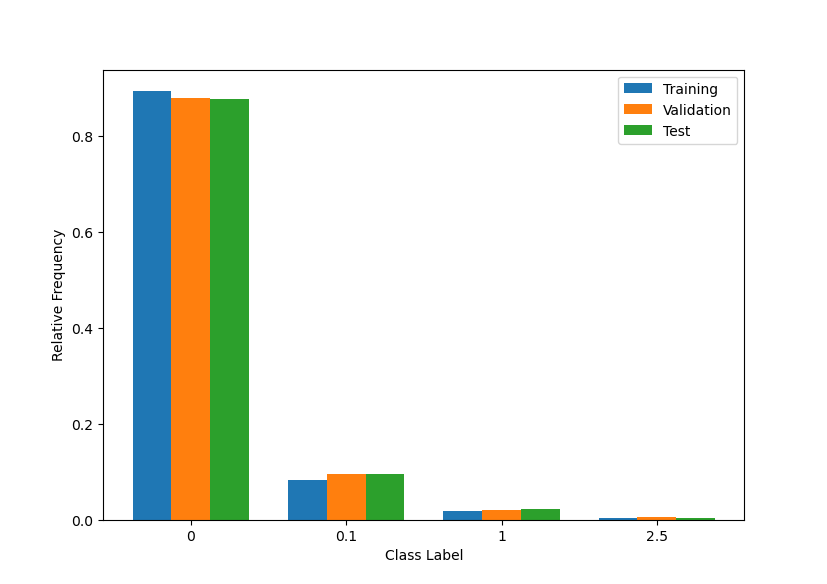
\includegraphics[width=0.9\textwidth]{Class Frequencies Bar.png}
    \caption{Bar chart of the precipitation class (see \cref{tab:prec_classes}) frequencies for training, validation and test subset of the dataset. The frequencies sum to 1 for each one of the subsets. The chart is computed using data from \cref{tab:classdistributions}.}
    \label{fig:classdistributions}
\end{figure}
\begin{table}[h]
    \centering
    \begin{tabular}{cccc}
    \hline
    \multicolumn{4}{c}{Scenes Selection} \\
    \hline
    \hline
         & Training & Validation & Test \\
    \hline
         Available Scenes & 63336 & 10176 & 10200 \\
         Selected Scenes & 58784 & 7116 & 7074 \\
         Percentage Selected & 92.8\% & 69.9\% & 69.3\% \\
         Proportion in Dataset & 80.6\% & 9.8\% & 9.7\% \\
         \hline
    \end{tabular}
    \caption{Breakdown of the selection of scenes from all the available scenes. The third row is computed by dividing the selected scenes by the available scenes. The proportion in the total dataset is computed by dividing the selected scenes by the sum of all selected scenes. A scene is discarded if and only if all the input frames are rainless.}
    \label{tab:rainydays}
\end{table}


\subsubsection{Weights for Training}
To counteract the class imbalance, using weights in the cross-entropy loss of the model is normally the preferred choice in the deep learning literature. These weights are typically the inverse of the frequency of the classes. That means, following the frequencies as reported in \cref{tab:classdistributions},
\begin{align*}
   & \text{Class 0} & \frac{1}{89.4} \\
   & \text{Class 0.1} & \frac{1}{8.34} \\
   & \text{Class 1.0} & \frac{1}{1.81} \\
   & \text{Class 2.5} & \frac{1}{0.42}
\end{align*}
Other methods of balancing a cross-entropy loss exist, such as the employment of an effective number of samples \citep{Cui2019Class-BalancedSamples} that builds upon the reasoning that as the number of samples increases, the additional benefit of a newly added data point diminishes.
\subsubsection{Skewness of inputs}
Knowing that high precipitation rates are infrequent and that in general very skewed distributions for the layers of a neural network are not desireable, I assess the frequency and shape of the distribution of the values for the raw precipitation rates of the RADOLAN dataset as those are the ones that are fed as input to the model. 

In order to make the distribution less skewed and bring it closer to a normal distribution, a common solution is to transform the data by taking the (natural) logarithm; for instance \citet{Ayzel2020RainNetNowcasting} decide to transform the input to the model by taking the natural logarithm as in
\begin{equation} \label{eq:transform}
    x_{\text{transformed}} = \ln(x_{raw} + 0.01)
\end{equation}
where 0.01 is added to the raw input to avoid the logarithm of zero. \cref{fig:trainfreq} shows the implication of this transformation for the distribution of the precipitation values.

\begin{figure}[!h]
    \centering
    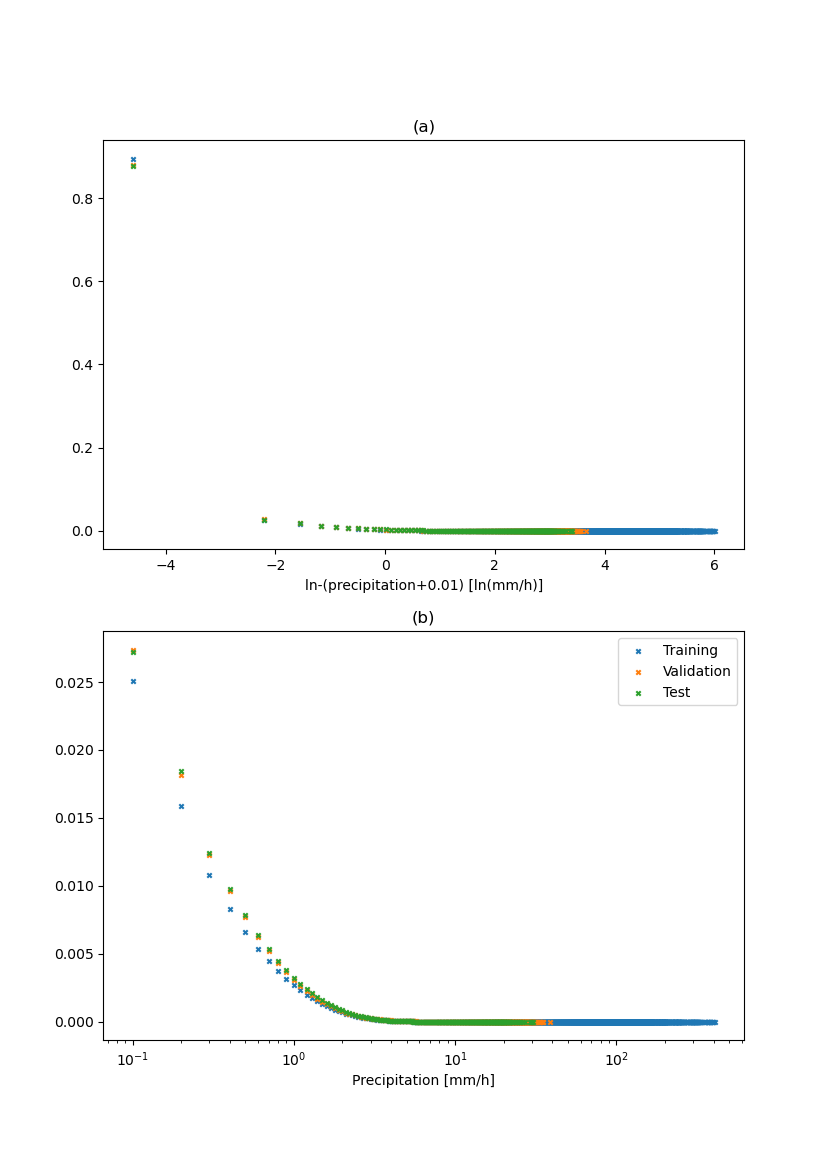
\includegraphics[width=0.9\textwidth]{figure_datasets.png}
    \caption{Relative frequency of all precipitation values for the pixels of the frames in the RADOLAN dataset. The distributions are computed for the training, validation ad test subsets of the dataset. (a) displays the distribution after the transformation of \cref{eq:transform}, hence the distribution of the values fed to the model. (b) is the distribution of the values displayed in log-scale without any addition but it does not contain the most frequent value 0 in order to better understand the distribution among the other values. }
    \label{fig:trainfreq}
\end{figure}


\section{Model Performance}
\subsubsection{Hyperparameter Search}\label{hyperparametersearch}
To avoid a computationally expensive procedure, the hyperparameters were divided in two groups. (1) Those manually tuned and (2) those picked by utilizing the available literature.

The manual search was done by trial and error considering all the metrics on the validation set, paying more attention to the HSS and the CSI. \cref{tab:hyperparameters} sums up the hyperparameters found through this process. 

\begin{table}[!h]
    \centering
    \begin{tabular}{cc}
        \hline
        \multicolumn{2}{c}{Hyperparameters} \\
        \hline
        \hline
         Name & Value \\
         batch size & 32 \\
         depth & 6 \\
         epochs & 10 \\
        \hline
    \end{tabular}
    \caption{The hyperparameters found via manual tuning.}
    \label{tab:hyperparameters}
\end{table}

\subsubsection{Testing}
Using the model produced through the hyperparameters of \cref{tab:hyperparameters} the metrics are computed on the testing subset. The results are summed up in \cref{tab:testing}

\begin{table}[!h]
    \centering
    \begin{tabular}{cccccc}
    \hline
    Metric & Cl. 0 & Cl. 0.1 & Cl. 1 & Cl. 2.5 & Macro average \\
     \hline
    \multirow{2}{*}{Precision} & \textbf{0.988} & 0.346 & \textbf{0.309} & 0.218 & 0.465 \\
         & 0.943 & \textbf{0.433} & 0.308 & \textbf{0.227} & \textbf{0.478}\\
    \hline
        \multirow{2}{*}{Recall} & 0.861 & \textbf{0.653} & \textbf{0.585} & \textbf{0.609} & \textbf{0.677} \\
         & \textbf{0.943} & 0.433 & 0.308 & 0.226 & 0.478 \\
    \hline
        \multirow{2}{*}{F1} & 0.921 & \bm{0.452} & \bm{0.404} & \bm{0.321} & \textbf{0.525} \\
         & \bm{0.943} & 0.432 & 0.308 & 0.227 & 0.478 \\
    \hline
        \multirow{2}{*}{CSI} & 0.853 & \bm{0.292} & \bm{0.253} & \bm{0.191} & \textbf{0.397} \\
         & \bm{0.893} & 0.276 & 0.182 & 0.128 & 0.370 \\
    \hline
        \multirow{2}{*}{HSS} & 0.579& 0.438 & \bm{0.404} & \bm{0.321} & \textbf{0.436} \\
         & \bm{0.583} & \bm{0.441} & 0.314 & 0.229 & 0.392 \\
    \hline
    \end{tabular}

    \caption{The results of the model compared to persistence applied to the test subset of the dataset. For every metric the upper row refers to the results of the model whilst the lower row refers to persistence. Higher values are better. The best values for each class and metric are highlighted.}
    \label{tab:testing}
\end{table}

As \cref{tab:testing} shows the performance of the model is generally better than persistence for higher precipitation classes suggesting an influence of the weights for the loss giving higher importance to higher precipitation. The generally high values for precision and recall for the lowest precipitation class can be explained by the overall higher amount of tiles with no precipitation making it an "easy guess". The most significant information is to be found in the overall better prediction skill of the model compared to persistence for the remaining classes as the macro-averages testify.

\begin{figure}[!h]
    \centering
    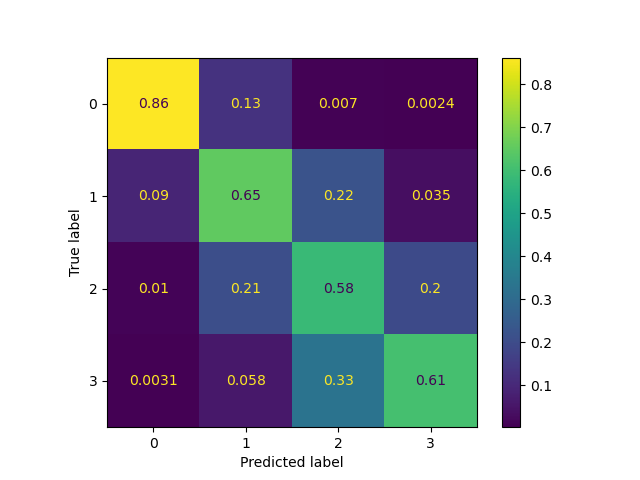
\includegraphics[width=0.9\textwidth]{normlized_confmatrix_test_2022-05-11 15:41:17.958023.png}
    \caption{The normalized confusion matrix for the predictions made by the model on the test set. Normalization occurs on the rows. The labels 0, 1, 2, 3 stand for the classes 0, 0.1, 1, 2.5 respectively.}
    \label{fig:confusion_matrix}
\end{figure}

\cref{fig:confusion_matrix} is the confusion matrix for the task. As it suggests the majority of wrong classifications happen with neighbouring classes, meaning that the model is able to understand the shape of the precipitation but has difficulties in assessing the intensity correctly.

\section{Case Studies}
To visually assess the goodness of the model I analyse two case studies, the first scene is the one at 2020-02-09T1950Z and the second one is at 2021-03-11T0150Z.

\subsection{First Case Study: 2020-02-09T1950Z}
\subsubsection{Synoptic Situation}
The synoptic situation near the time of the input and output of the neural network is addressed through the use of the model results produced by NOAA's model Global Forecast System (GFS)\footnote{https://www.ncei.noaa.gov/products/weather-climate-models/global-forecast} and visualized through Ertel2\footnote{http://ertel2.uibk.ac.at:8080/}. Geopotential height and equivalent potential temperature at 850hPa are employed. \cref{fig:ertel1} shows the relative figure for the model output at 2020-02-10T0000Z where the presence of a cold front is evident in the northern part of Germany near the area of interest (cf. \cref{fig:area_selection}). The orientation of the front is SW-NE. Additionally, given the orientation of the isolines representing the geopotential, the direction of the geostrophic flow is easterly. I also assess the 1h accumulated precipitation associated with this front by observing the output of the ICON (EU) model\footnote{more on the ICON (EU) model to be found at \newline \hyperlink{https://www.dwd.de/EN/ourservices/nwp\_forecast\_data/nwp\_forecast\_data.html}{https://www.dwd.de/EN/ourservices/nwp\_forecast\_data/nwp\_forecast\_data.html}} through Ventusky\footnote{\hyperlink{https://www.ventusky.com/}{https://www.ventusky.com/}} at 2020-02-10T0300Z. \cref{fig:ventusky1} shows the relative image. The precipitation bands near the area of interest in northern Germany (again cf. \cref{fig:area_selection}) are oriented in a similar direction to the cold front i.e. SW-NE.
\begin{figure}[!h]
    \centering
    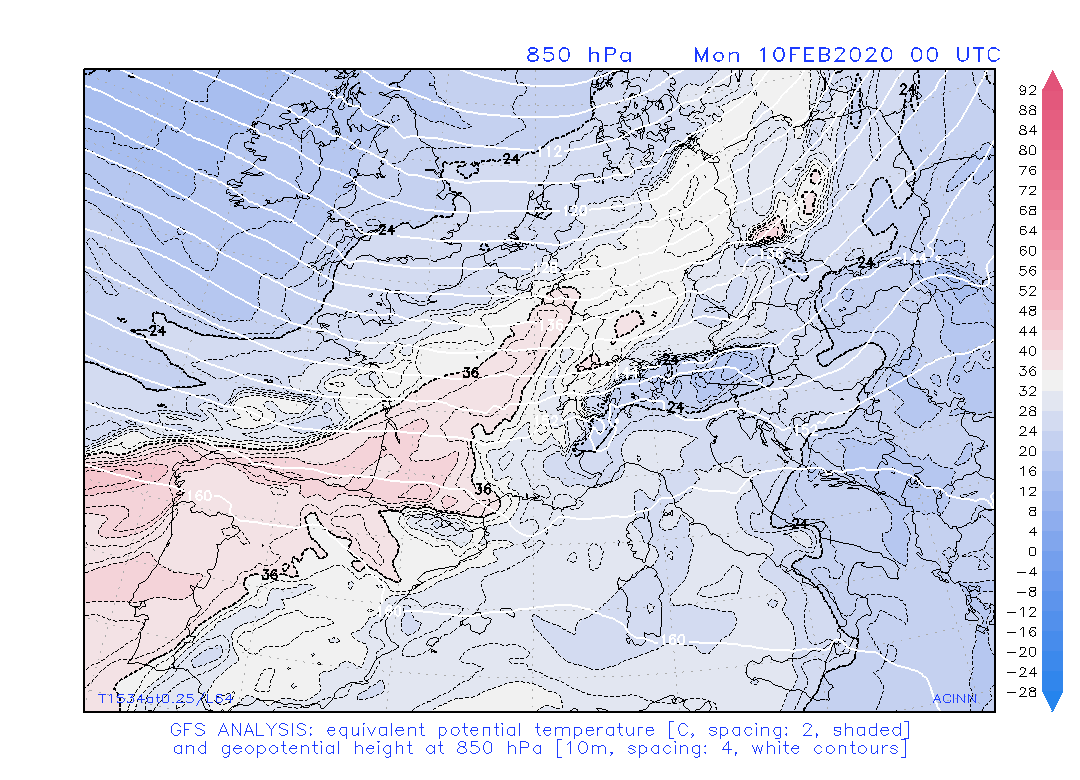
\includegraphics[width=0.9\textwidth]{2002100000_gfs.png}
    \caption{Output of the GFS model for the timestamp 2020-02-10T0000Z showing equivalent potential temperature and geopotential height at 850hPa. The equivalent potential temperature is in C, shaded and with lines at 2\textdegree C distance. The geopotential height is shown in white contours and in 10m units. The spacing between the lines is 4. The SW-NE cold front in the area of interest in norther Germany is evident. The flow is assessed through the geopotential height and is easterly. Figure produced with the help of ERTEL2.}
    \label{fig:ertel1}
\end{figure}
\begin{figure}
    \centering
    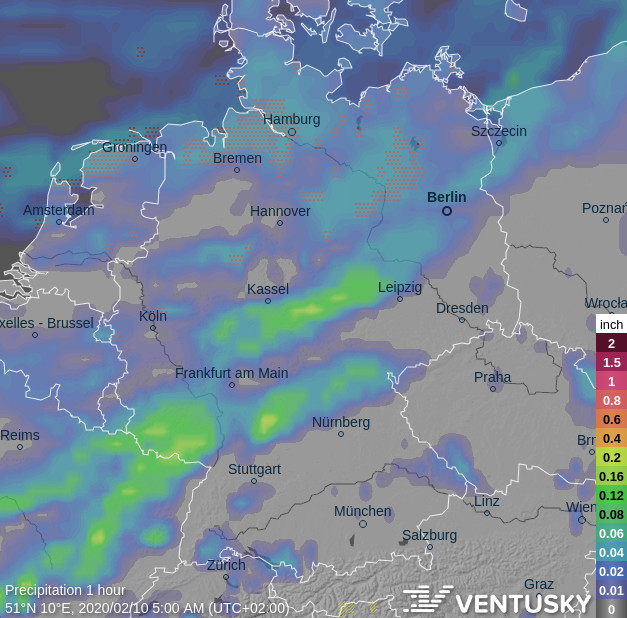
\includegraphics[width=0.9\textwidth]{ventusky-rain-1h-20200210t0300-51n10e.jpg}
    \caption{1h precipitation over Germany at 2020-02-10T0300Z according to the ICON (EU) model. The frontal structure after it has passed over the area of interest and its approximate SW-NE orientation can be seen clearly. Figure produced with Ventusky.}
    \label{fig:ventusky1}
\end{figure}

\subsubsection{Model Prediction}
Following the synoptic situation described in the previous section I analyze the actual output of the model given the input sequence. \cref{fig:examplescene1} shows the scene for 2020-02-09T1950Z. This timestamp is the timestamp of the first input image (upper left in the group of 6 images). The other 5 input images are those depicted in the group made of 6 images in \cref{fig:examplescene1} and all are of precipitation accumulated in a 1h interval. They are separated by 1h from each other. The model then applies a series of convolutions (cf \cref{sec:convolutional_layers}) that abstract the features of the input images in a representational space that the model itself learns during the training process. The spatial resolution is reduced for every layer that the input data goes through in the encoding phase (cf. \cref{sec:Unet}) but is later taken back to the original resolution in the decoding phase. In this last phase the model rebuilds a plausible output image using information from the encoding phase thanks to the skip connections (cf. \cref{sec:skip_connections}). The timestamp of the output of the model is 6h after the first input image, hence 2020-02-10T0150Z and it is shown in the last row on the left of \cref{fig:examplescene1}, it is confronted with the ground truth on the same row on the right. This allows for a straightforward comparison and shows if the model has acquired the ability to infer the spatial distribution of the precipitation correctly. As \cref{fig:examplescene1} shows the model is indeed able to predict precipitation rainbands going in the SW-NE direction as is seen in the ground truth and in \cref{fig:ventusky1}. However, it is clear that the model predicts higher precipitation rates than are actually observed. An hypothesis for this behaviour is the influence of the weights employed for the loss that give very high importance to higher precipitation rates.
\begin{figure}[!h]
    \centering
    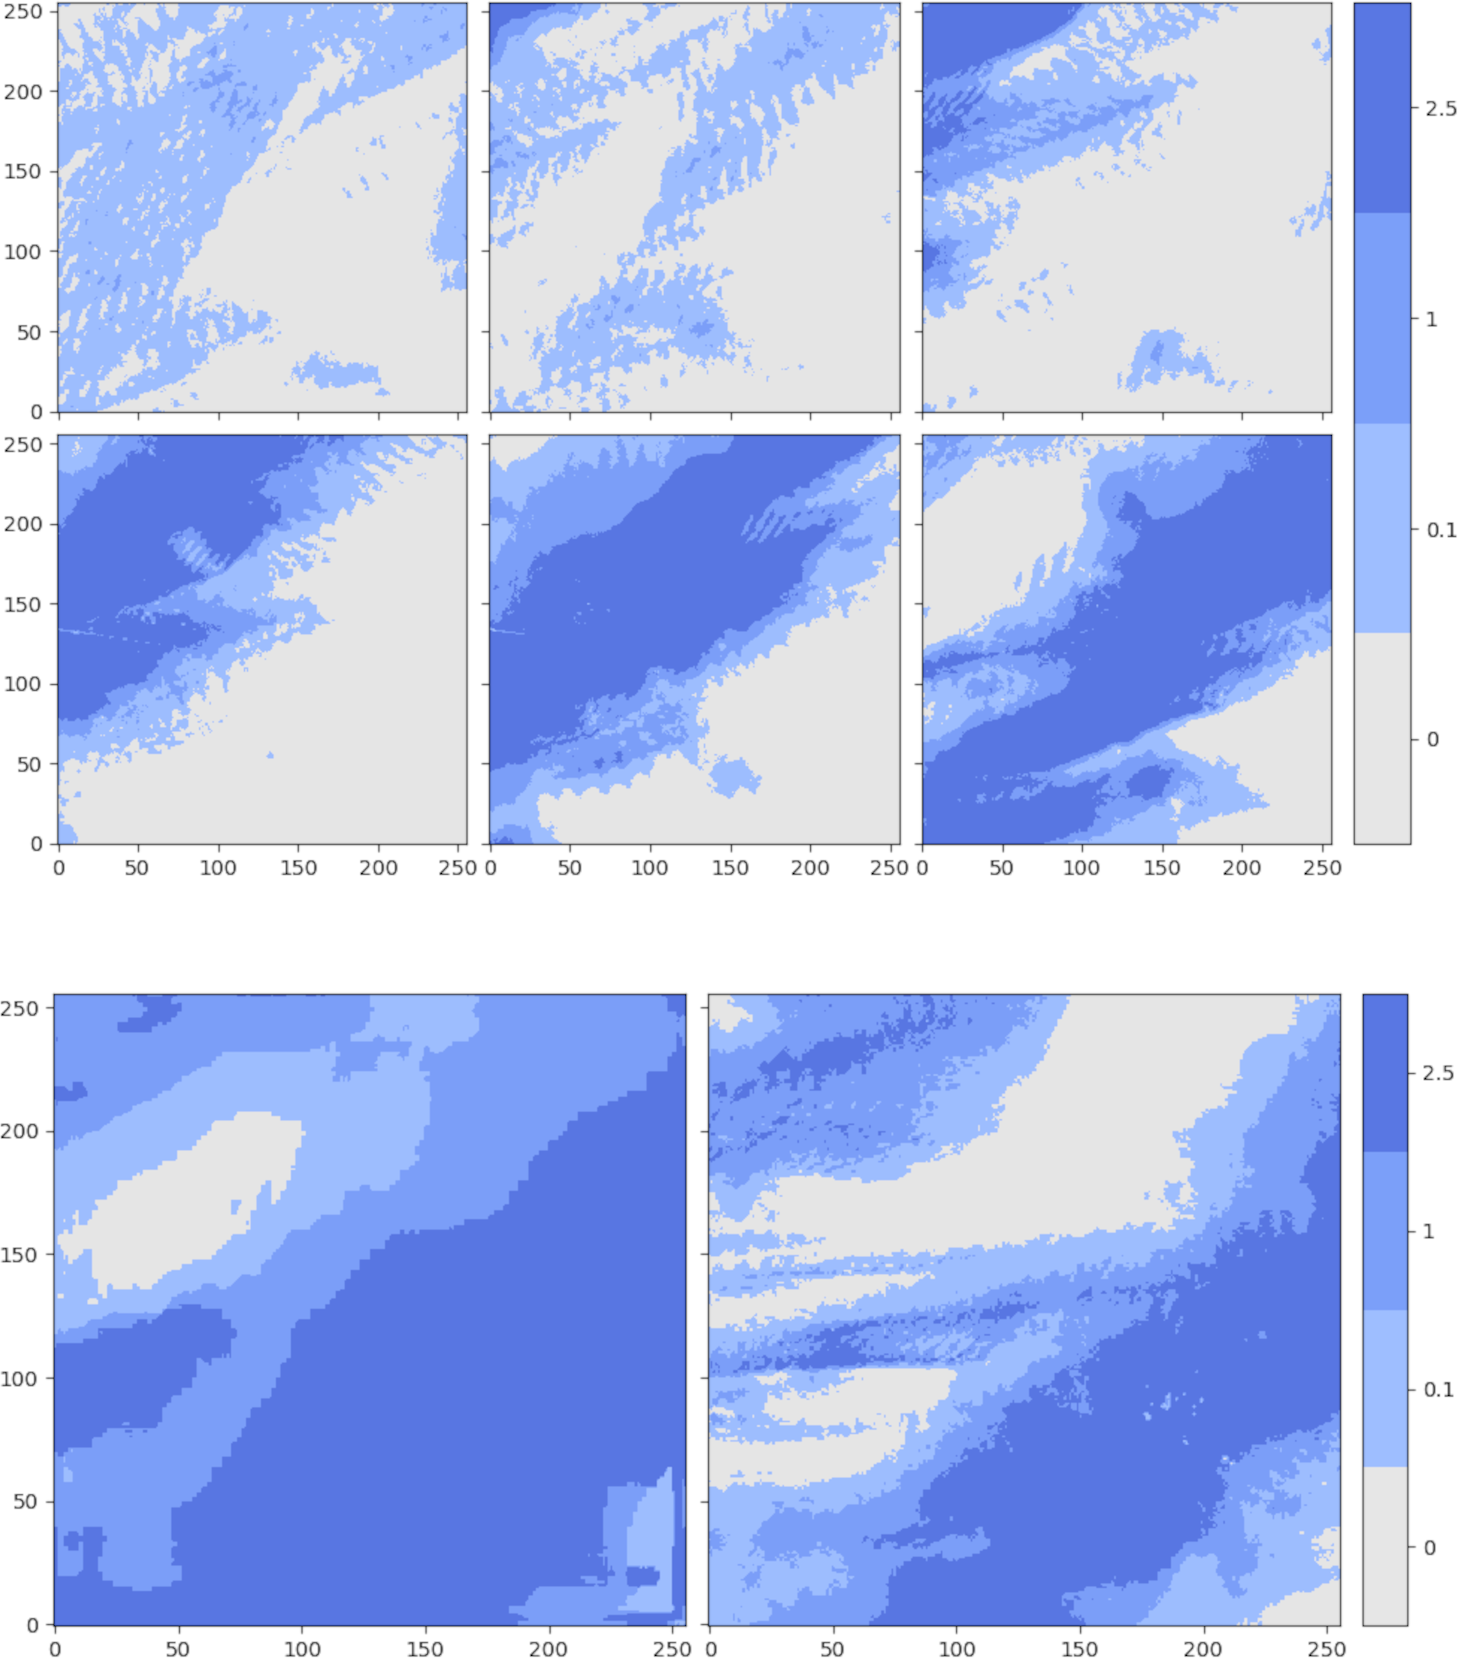
\includegraphics[width=0.9\textwidth]{2002091950.png}
    \caption{Example of input and output and ground truth for 2020-02-09T1950Z. The input part is made of the six images in the top. The prediction is the left image of the lower two and the ground truth is to be found on the right of the prediction. The input is fed to the model as continuous precipitation values but it is depicted in precipitation classes to better compare them with the output. The labels on the right refer to the precipitation classes. The coordinates are in km from the bottom left corner. The order of the inputs is left to right top to bottom. The interval between every one is one hour and all are 1h cumulative precipitation values. The model can be seen to correctly predict the orientation of the precipitation bands. At the same time it predicts higher precipitation values than the ground truth.}
    \label{fig:examplescene1}
\end{figure}

\subsection{Second Case Study: 2021-03-11T0150Z}
\subsubsection{Synoptic Situation}
Similarly to the first case study, I assess the synoptic situation at a time approximately near to the input and output of the neural network (the latter is 6h after the input image, hence 2021-03-11T0750Z) using the same tools. \cref{fig:ertel2} shows the output of GFS and shows the presence of a warm front that is starting to enter the area of interest in northern Germany at 2021-03-11T0000Z. Its orientation is S-N. The geostrophic flow associated to the system, being parallel to the isolines of geopotential height, is found to be easterly to south-easterly. The rainbands associated with this front can be seen in the ICON (EU) model output taken at 2021-03-11T0900Z after they have left the area of interest and are in the SW-NE direction.
\begin{figure}[!h]
    \centering
    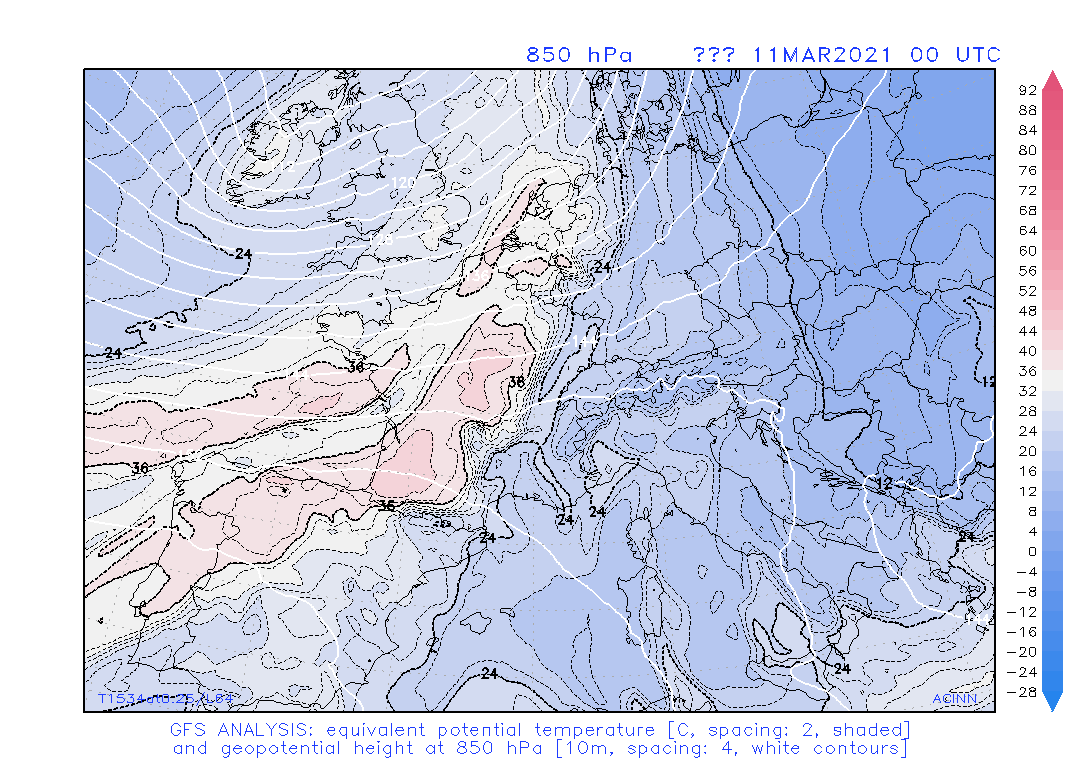
\includegraphics[width=0.9\textwidth]{2103110000_gfs.png}
    \caption{Output of the GFS model for the timestamp 2020-03-11T0000Z showing equivalent potential temperature and geopotential height at 850hPa. The equivalent potential temperature is in C, shaded and with lines at 2\textdegree C distance. The geopotential height is shown in white contours and in 10m units. The spacing between the lines is 4. The N-S warm front approaching the area of interest in northern Germany is evident. The geostrophic flow, parallel to the isolines of geopotential height, is easterly to south-easterly. Figure produced with the help of ERTEL2.}
    \label{fig:ertel2}
\end{figure}
\begin{figure}
    \centering
    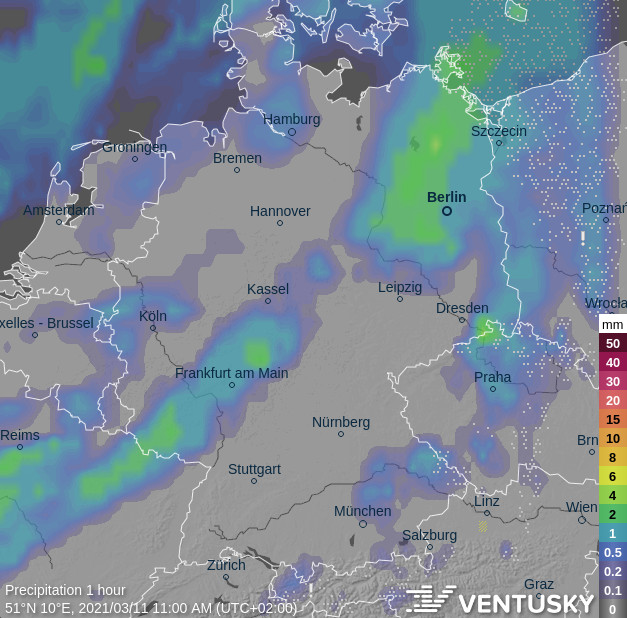
\includegraphics[width=0.9\textwidth]{ventusky-rain-1h-20210311t0900-51n10e.jpg}
    \caption{1h precipitation over Germany at 2021-03-11T0900Z according to the ICON (EU) model. The frontal structure after it has passed over the area of interest can be seen over northern Germany. Its orientation is SW-NE. Figure produced with Ventusky.}
    \label{fig:ventusky2}
\end{figure}

\subsubsection{Model Prediction}
Following the synoptic situation, I assess again the ability of the model to predict high level features such as the direction of the precipitation bands. I find in \cref{fig:examplescene2}, similarly to the first case, that the model is able to predict the direction of the precipitation bands but outputs higher precipitation rates than the ground truth.
\begin{figure}[!h]
    \centering
    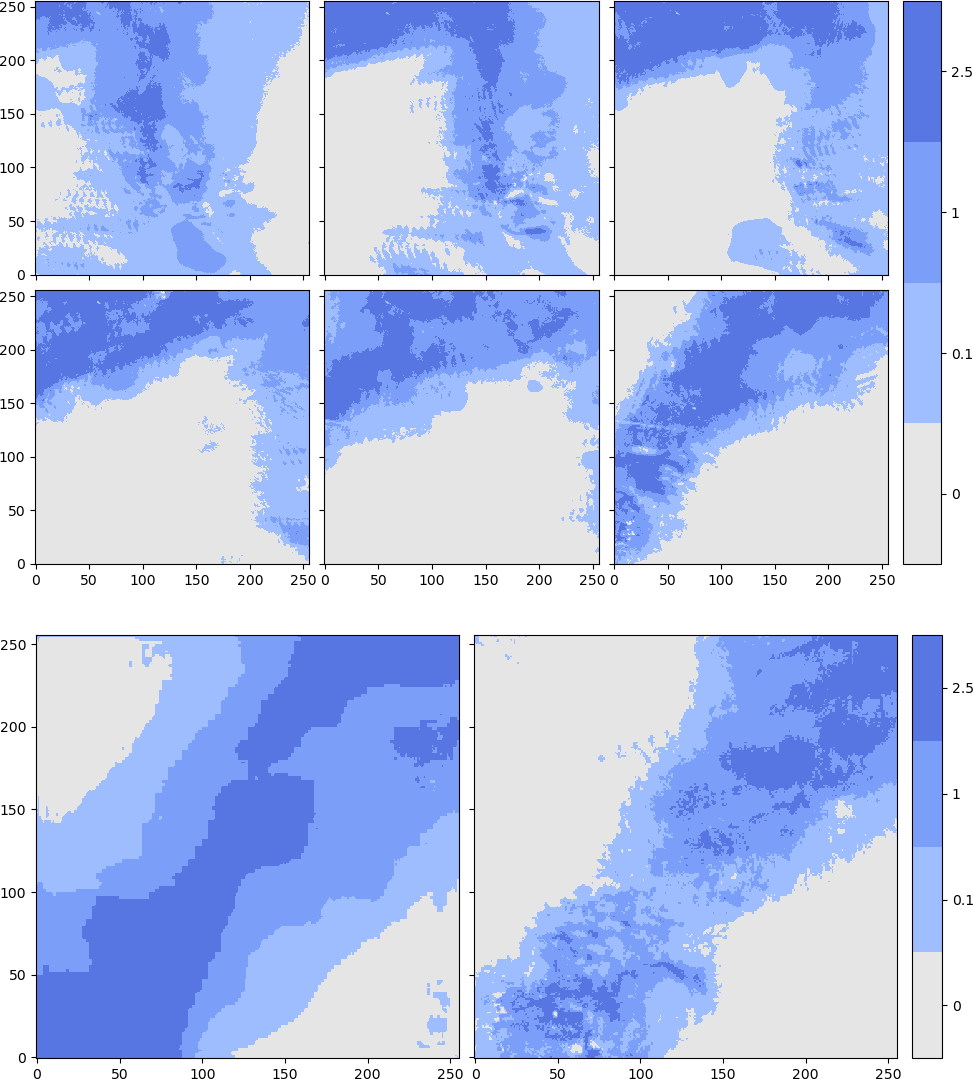
\includegraphics[width=0.9\textwidth]{2103110150.png}
    \caption{Example of input and output and ground truth for 2021-03-11T0150Z. The input part is made of the six images in the top. The prediction is the left image of the lower two and the ground truth is to be found on the right of the prediction. The input is fed to the model as continuous precipitation values but it is depicted in precipitation classes to better compare them with the output. The labels on the right refer to the precipitation classes. The coordinates are in km from the bottom left corner. The order of the inputs is left to right top to bottom. The interval between every one is one hour and all are 1h cumulative precipitation values. The model can be seen to correctly predict the orientation of the precipitation bands. At the same time it predicts higher precipitation values than the ground truth.}
    \label{fig:examplescene2}
\end{figure}


\newpage
\thispagestyle{plain}


% ==== DISCUSSION and CONCLUSIONS ===============================================
% ---- set some counters to zero:
\setcounter{equation}{0}
\setcounter{table}{0}
\setcounter{figure}{0}
% ---- include tex-file:
\chapter{Discussion and Conclusions}\label{chap4}
\thispagestyle{plain}
 In this chapter I will discuss the results by answering the research questions followed by a part on the decision taken for the methodology. Finally, I will compare the results with similar studies and state some possible developments.
\section{Results}

The answers to the research questions of \cref{sec:researchquestions} follow:
\begin{enumerate}
    \item \textbf{Does the employed neural network outperform persistence?} For most of the metrics and classes the neural network outperforms persistence. This is also what the macro-averages indicate. The macro averaged HSS for the neural network is 0.436 compared to 0.392 for persistence. The macro-averaged CSI is 0.397 for the neural network compared to 0.370 for persistence.
    \item \textbf{How does the model's performance depend on the rainfall intensity?} The performance of the model, in absolute terms decreases with rainfall intensity but gets generally better compared to persistence for increasing rainfall intensity.
    \item \textbf{The model of \citet{Agrawal2019MachineImages} after which this project is inspired outperformed persistence for all precipitation classes. Can this result be confirmed?}
    The model of this thesis was also found to generally outperform persistence albeit not to the same degree as the original paper. However, the ability of the model to abstract features as indicated by \cref{fig:examplescene1,fig:examplescene2} suggests that with further hyparameter tuning a similar performance could be achieved.
    \end{enumerate}



% ==== Section 1 ============================================================
\section{Discussion of the Methodology}
In this section I will discuss the decisions taken as regards to the methodology.

\subsection{Choice of the Network Architecture}
The network architecture of this project is chosen to resemble the ubiquitous U-Net architecture introduced by \citet{Ronneberger2015U-Net:Segmentation} that was found to perform well on segmentation tasks. As for the particular details of the various layers composing the network, I followed \citet{Agrawal2019MachineImages}. I treated the model depth as a hyperparameter given that \citet{Ayzel2020RainNetNowcasting}, trying to solve a similar problem, adopts a depth of 4 (instead of 7 as in \citet{Agrawal2019MachineImages}. An advantage of lower depth is decreased memory footprint and computational requirements. However, not enough parameters can affect the model performance. Unfortunately, \cite{Agrawal2019MachineImages} are not exhaustive in their description of the architecture. The lacking information was compensated by adopting solutions available in the general deep learning literature. The architecture of short-range skip connections when downsampling blocks are applied and the number of input feature maps to the blocks are different from the number of output feature maps \citep{Drozdzal2016TheSegmentation}. 

\subsection{Changes in the RADOLAN Routine}
The RADOLAN calibration routine described in \cref{sec:radolan} is subject to constant changes that are brought into the operational procedure. \citet{Weigl2021RADOLANRoutine} keeps track of these changes. Some are as as simple as additional ground rain gauges or the dismissal and addition of radar stations. Other changes affect the algorithm of the routine itself, such as better corrections for the shadowing of radar signals by the orography. The DWD has until now reprocessed the RADOLAN database twice, these data are available and could be used to improve the model performance.

\subsection{Choice of the Training, Validation and Test Sets}
It is common practice in the artificial intelligence literature to subdivide the dataset into three subsets, the training set used for optimizing the model, the validation set to compare the different hyperparameter choices and the test set to produce the final data later reported as the actual performance of the model. The proportions 80:10:10 are common choice for deep learning tasks. The choice of chronological order was taken partly also considering the changes in the RADOLAN calibration procedure, hence allowing the final performance measure to be closer to the performance if the model were to be applied to very recent data. A significant drawback of this approach is that it relies on the assumption that the time-series is stationary, i.e. no changes occurred to the underlying processes, in this case the climate. An alternative way to asses model performance avoiding the use of the computationally expensive cross validation, would be to choose the training set by randomly selecting members of the dataset.

\subsection{Area and Time-Resolution Selection}
Orography is known to introduce error in the final product derived from radar reflectivity measurements. For simplicity and to remain within the investigative and non-operational nature of the project I decided to select a limited area in a flat region of Germany completely within the RADOLAN RW product's domain. As it pertains to the choice of 1hr cumulative precipitation data, this was driven by the lack of literature applying deep learning weather prediction at those timescales. \citet{Agrawal2019MachineImages} uses 7 images at 10min distance from each other taken from the multi radar multi sensor (MRMS) dataset and predicts the MRMS image at 1h after the last image of the input. \citet{Ayzel2020RainNetNowcasting} in contrast uses 4 images at 5min interval from the RADOLAN RY product to predict a similar image 5min after the last one of the input series.

\subsection{Alternative Comparisons}
The model in this thesis was compared only with the so-called persistence prediction that works by assuming that the forecast is equal to the data at the last available time before the forecast. Despite its simplicity, persistence is not a trivial prediction to outperform and serves as first intuitive benchmark to understand the performance of a prediction method. \citet{Agrawal2019MachineImages} after which this thesis is partly inspired, compared their model with both persistence and the HRRR model. \citet{Ayzel2020RainNetNowcasting} too compared their model against persistence. They also compared it with the results of the \verb|rainymotion| \citep{Ayzel2019OpticalV0.1} optical flow library albeit at a 5min time resolution. The \verb|rainymotion| library was shown to outperform the RADVOR \citep{DeutscherWetterdienst2022RADVORRadar-Niederschlagsvorhersage} operational nowcast model of the DWD \citep{Ayzel2019OpticalV0.1}. Given the similarity of the dataset between this study and \citet{Ayzel2020RainNetNowcasting} further comparisons could include the accumulated hourly product produced by the RADVOR nowcast. The application of an optical flow algorithm such as \verb|rainymotion| to the 1h accumulated rainfall data needs to be investigated.

\subsection{Hyperparameters Optimization}
For the optimization of the hyperparameters of the model, I applied the manual search using knowledge guided by the literature as regards to the most plausible hyperparameter choice. As discussed in \cref{sec:hyperparametersearch} different methods to find the best combination of hyperparameters exist. It is likely that the application of an algorithm such as random search \cite{Bergstra2012RandomOptimization} could improve the results. However, considering the investigative purpose of this project, the increased amount of time and resources needed to train the model with multiple hyperparameters combinations would be beyond the current scope.

\subsection{Class Imbalances}
An imbalanced dataset is a common problem in classification tasks. The relevance is even more pronounced if the less frequent class is also of higher importance. For this project, as shown in \cref{tab:classdistributions} the high precipitation classes are vastly underrepresented in the dataset compared to the dominant no-rainfall class. The solution I employed, following a common practice in the deep learning community is to assign weights proportional to the inverse of the frequency of the classes for the purpose of computing the loss. However, this choice seems to lead to an overprediction of high rainfall classes. The choice of weights can be considered as part of hyperparameter tuning. A possible alternative way to address the class imbalance problem would be to adopt so-called effective number of samples \citet{Cui2019Class-BalancedSamples} that tries to to capture the diminishing marginal benefits by using more
data points of a class allowing for less compensation of the imbalance.


% ==== Section 3 ============================================================
\section{Comparison with Similar Studies}

The literature on precipitation nowcasting is fairly recent and therefore the available studies are somewhat limited in number and scope. Nonetheless, some studies that focus on a task similar to the one addressed in this thesis exist. In these studies the precipitation nowcasting problem is almost always addressed at a time resolution of 5min between each input frame. \citet{Agrawal2019MachineImages} and \citet{Ayzel2020RainNetNowcasting} propose a network architecture (U-Net) and study setup most similar to the one of this project. They both found better performance of their respective models for their tasks compared to persistence, this result remained for increasing lead times in the case of \citet{Ayzel2020RainNetNowcasting} where the output of the model was used as input for subsequent frames. The two studies compared the U-Net to the HRRR model and optical flow respectively with input frames 10min and 5min apart. Such a comparison (i.e. a comparision with a a model used in operational settings) could not be made for the neural network used in this thesis but it is reasonable to assume that with better hyperparameter tuning and small changes to the architecture a similar result could be achieved.

\citet{Shi2017DeepModel} propose a recurrent architecture based on long and short term memory (LSTM) called TrajGRU. The peculiarity of the model is to learn the connection structure between the hidden states. It utilizes the current input and the previous state to generate a local neighbourhood that should influence a certain location at a every timestamp. The model was compared to traditional Convolutional Neural Networks and to the predecessor of TrajGRU: ConvGRU. In an offline setting a comparison with persistence and the model was made. In all cases the absolute performance of the model decreases as the precipitation rate increases. TrajGRU was found to always outperform all other models as well as persistence.

In the study by \citet{Ravuri2021SkillfulRadar} the authors test a Generative Adversarial Network (GAN) architecture against three competitive models: a U-Net implementation, PySTEPS \citep{Pulkkinen2019Pysteps:v1.0} and an implementation of MetNet \citep{Snderby2020MetNet:Forecasting}. The GAN consists of two parts, a generator and a discriminator. The generator is responsible for creating images (given an input) that should be as similar as possible to the ones in the dataset. The discriminator has to learn to distinguish between a real example and a generated one. \citet{Ravuri2021SkillfulRadar} showed that the GAN is chosen by expert forecasters from the Met Office as the one with the highest usefulness compared to the alternative proposed models. 

Overall the studies suggest that the deep learning perspective is a promising approach to the precipitation nowcasting problem. In this regard this thesis confirms the identified trajectory and warrants further investigation into the application of neural networks to the 1h time scale. Possible extensions include the study of the behaviour of a U-Net with additional input frames, additional physical variables other than precipitation, additional output frames, the utilization of the model outputs as inputs for extending the lead time of the prediction (as in \citet{Ayzel2020RainNetNowcasting}). All these developments have as a precondition the betterment of the current model, specifically with better hyperparameter tuning and a different weighting strategy for the various precipitation classes.
\newpage
\thispagestyle{plain}


% ==== CONCLUSIONS =============================================================
% ---- set some counters to zero:
% \setcounter{equation}{0}
% \setcounter{table}{0}
%\setcounter{figure}{0}
%  ---- include tex-file:
% \chapter{Conclusions}\label{concl}
\thispagestyle{plain}

This chapter contains consequences that derive from your results. It may also
contain speculations. It may provide suggestions for future studies. Hence, the
conclusions may provide an outlook and list open questions. Sometimes
this chapter is part of the discussion. In such a case, the chapter reads
``Discussion and Conclusions''.

% \newpage
% \thispagestyle{plain}


% ==== APPENDIX ================================================================
% ---- start appendix:
\appendix
% ---- set some counters to zero:
\setcounter{equation}{0}
\setcounter{table}{0}
\setcounter{figure}{0}
% ---- include tex-file:
\chapter{Software and Hardware}\label{appA}
\thispagestyle{plain}

The software was written in \textit{Python 3.8}. The RADOLAN dataset was handled through \textit{wradlib} \citep{Muhlbauer2022Wradlib/wradlib:V1.15.0}, \textit{xarray} \citep{Hoyer2022Xarray}, \textit{dask} \citep{DaskDevelopmentTeam2016Dask:Scheduling} and \textit{zarr} \citep{Miles2020Zarr-developers/zarr-python:V2.4.0}. The confusion matrix was done with the help of \textit{scikit-learn} \citep{Pedregosa2011Scikit-learn:Python}. The majority of the plots are produced with \textit{matplotlib} \citep{Caswell2019Matplotlib/matplotlib:V3.1.1} unless specified otherwise. The deep learning library used is \textit{Pytorch} \citep{Paszke2019PyTorch:Library} wrapped within \textit{Pytorch-Lightning} \citep{Falcon2020PyTorchLightning/pytorch-lightning:Release}. The computations partly happend on the Vienna Scientific Cluster\footnote{\hyperlink{https://vsc.ac.at//systems/}{https://vsc.ac.at//systems/}} 4 (VSC4) compute nodes, partly on VSC3 using the GPU nodes and partly on Google Compute Cloud.
\newpage
\thispagestyle{plain}


% ==== START BACK MATTER (this has no visual effect)============================
\backmatter 


% ==== BIBLIOGRAPHY ============================================================
\addcontentsline{toc}{chapter}{Bibliography}
% ---- use AMS reference format (use file ametsoc.bst included in ...
%      ... http://www.ametsoc.org/pubs/journals/AMS_Latex_V3.0.tar.gz):s
\bibliographystyle{./ametsoc}   % ametsoc.bst in local directory
% ---- use BibTeX database file:
\bibliography{./references}      % mybibfile.bib in local directory
\newpage
\thispagestyle{plain}


% ==== ACKNOWLEDGMENTS =========================================================
% ---- include tex-file:
\chapter*{Acknowledgments}
\addcontentsline{toc}{chapter}{Acknowledgments}
\thispagestyle{plain}

I would like to thank my incredible supervisor Prof. Georg Mayr for the continuous help and advice on every part of the thesis. Thank you for your support. I'd also like to thank Matthias Göbel, Daniel Frisinghelli and Prof. Haltmeier for the suggestions on the neural network. Thanks to all my classmates, especially to Michele Giurato, for having shared with me this very important part of my life. I'm grateful to my family, for them being by my side. Most importantly thank you to Gabi, for having helped me in finding new energy when everything seemed lost.  
\newpage
\thispagestyle{plain}

\end{document}
% ==== END OF BODY =============================================================
